%% Last modified: Time-stamp: <2010-07-27 14:23:51 (srdbadmin)>
%%\documentclass[letterpaper,12pt]{article}
\documentclass[letterpaper,review,authoryear,12pt]{myelsarticle}
%%\documentclass[preprint,authoryear,12pt]{elsarticle}

\usepackage{amssymb}
\usepackage{pdflscape}
\usepackage{longtable}
\usepackage{graphicx}
\usepackage{paralist}
\usepackage{comment}
\usepackage{color}
\usepackage[left=3cm,top=3cm,right=3cm, bottom=3cm,nohead]{geometry}
\usepackage{booktabs}
\usepackage{url}
%\usepackage[left,running]{lineno}
%\linenumbers
%\title{Assessing the knowledge-base for commercially exploited marine fishes and invertebrates with a new global database of stock assessments}

%%%\title{Assessing the knowledge-base for commercially exploited marine fishes and invertebrates with a new global database of stock assessments \\ \vspace{0.5cm} Alternative Title 1: A new global stock assessment database for exploited marine species \\ \vspace{0.5cm} Alternative Title 2: Understanding marine population dynamics using a new global database \\ \vspace{0.5cm} Suggested Running Title: A new global stock assessment database}

%\author{
%Daniel Ricard \thanks{Department of Biology, Dalhousie University, Halifax, NS B3H 4J1, Canada} \and 
%C{\'o}il{\'i}n Minto \and 
%Julia Baum\thanks{Scripps Institution of Oceanography, UCSD, 9500 Gilman Drive, La Jolla, CA 92093-0202, USA} \and 
%Olaf Jensen \thanks{School of Aquatic and Fishery Sciences, University of Washington, Seattle, WA  98195-5020, USA}
%}

\begin{document}

\begin{frontmatter}

%% Title, authors and addresses

%% use the tnoteref command within \title for footnotes;
%% use the tnotetext command for the associated footnote;
%% use the fnref command within \author or \address for footnotes;
%% use the fntext command for the associated footnote;
%% use the corref command within \author for corresponding author footnotes;
%% use the cortext command for the associated footnote;
%% use the ead command for the email address,
%% and the form \ead[url] for the home page:
%%
%% \title{Title\tnoteref{label1}}
%% \tnotetext[label1]{}
%% \author{Name\corref{cor1}\fnref{label2}}
%% \ead{email address}
%% \ead[url]{home page}
%% \fntext[label2]{}
%% \cortext[cor1]{}
%% \address{Address\fnref{label3}}
%% \fntext[label3]{}

\title{RAM Legacy: a new global stock assessment database for exploited marine species
\\ \vspace{0.5cm} \small Alternative Title 1: Assessing the knowledge-base for commercially exploited marine fishes and invertebrates with a new global database of stock assessments
\\ \vspace{0.5cm} Alternative Title 2: Understanding marine population dynamics using a new global database 
\\ \vspace{0.5cm} \normalsize Suggested Running Title: A new global stock assessment database \vspace{1.5cm}}

%% use optional labels to link authors explicitly to addresses:
%% \author[label1,label2]{<author name>}
%% \address[label1]{<address>}
%% \address[label2]{<address>}

\normalsize
\author[dal]{Daniel Ricard\corref{cor1}}
\ead{ricardd@mathstat.dal.ca}
\author[dal]{C{\'o}il{\'i}n Minto\fnref{fn2}}
\author[scripps]{Julia Baum\fnref{fn3}}
\author[uw]{Olaf Jensen\fnref{fn4}}
\cortext[cor1]{Corresponding author: Tel: 902-494-2146, Fax: 902-494-3736} 
\fntext[fn2]{Current Address: Marine and Freshwater Research Centre, Galway-Mayo Institute of Technology, Dublin Road, Galway, Ireland}
\fntext[fn3]{Current Address: National Center for Ecological Analysis and Synthesis, UCSB, 735 State St. Suite 300, Santa Barbara, CA 93101, USA}
\fntext[fn4]{Current Address: Institute of Marine and Coastal Sciences, Rutgers University, 71 Dudley Road, New Brunswick, NJ 08901-8525, USA}

\address[dal]{Department of Biology, Dalhousie University, Halifax, NS B3H 4J1, Canada}
\address[scripps]{Scripps Institution of Oceanography, UCSD, 9500 Gilman Drive, La Jolla, CA 92093-0202, USA}
\address[uw]{School of Aquatic and Fishery Sciences, University of Washington, Seattle, WA  98195-5020, USA}


%\begin{abstract}
%% Text of abstract
%%%%%%%%%%%%%%%%%%%%%%%%%
%% Abstract
%%%%%%%%%%%%%%%%%%%%%%%%% 
%%\newpage
\section*{Abstract}

Data used to assess the status of individual fish stocks varies from
very little information on many of the world's artisanal fisheries, to
commercial landings, research surveys, and sophisticated population
dynamics models that integrate many sources of information.  Previous
evaluations of the state of global fisheries have used catch data,
which may be poor proxies for fish stock abundances. A global
compilation of stock assessment data in the mid-1990s enabled
substantial syntheses of stock status; however its focus was on
stock-recruitment relationships and it is now 15 years out of date. To
facilitate contemporary syntheses, we have assembled a new database,
the RAM Legacy Database, of the most intensively studied commercially
exploited marine fish stocks, including time series of total biomass,
spawner biomass, recruits, fishing mortality, and catch; reference
points; and ancillary information on the life history, management, and
assessment methods for each stock.  Here, we present the first
overview of this database and use it to evaluate the knowledge-base
for assessed marine species.  Assessments were assembled for
323 stocks (287 fish species
representing 45 families, and
36 invertebrate species representing
12 families), including 8 of the world's 10
largest fisheries. Assessments were obtained from 18 national and
international management institutions, with most coming from North
America, Europe, Australia, New Zealand and the high seas.  Overall,
58\% of stocks are below $B_{msy}$, and 30\% have exploitation levels above
$U_{msy}$.  Assessed marine fish stocks comprise a relatively small
proportion of harvested taxa (24\%), and an even smaller proportion of
marine fish biodiversity (1\%).


%Globally, stock assessments were found
%for 323 stocks (287 species
%of fishes representing 45 families and
%36 species of invertebrates representing
%12 families), from 18
%national and international
%management institutions.

\noindent Keywords: marine fisheries, meta-analysis, population dynamics models, relational database, stock assessment, synthesis.

%with XX\% coming from north temperate regions (North
%Atlantic, North Pacific)
%\noindent Keywords: marine fisheries, meta-analysis, population dynamics models, relational database, stock assessment, synthesis.
%\newpage

%  Geographic differences in assessment
%methods show that Statistical Catch at Age (SCA) models are widely
%used by the west coast of the U.S. (XX percent of assessments),
%regional fishery management organizations in the Pacific (XX percent
%of assessments), and New Zealand (XX percent of assessments); the east
%coast of the U.S. is transitioning from Virtual Population Analysis
%(VPA) to SCA (XX percent of assessments conducted since 2000 have used
%SCA); while VPA is still the dominant assessment
%technique in western Europe (XX percent of assessments).


%\end{abstract}

%\begin{keyword}
%marine fisheries \sep meta-analysis \sep population dynamics models \sep relational database \sep stock assessment \sep synthesis
%\end{keyword}

\end{frontmatter}


\newpage
%\newpage
\section*{Abstract}

Data used to assess the status of individual fish stocks varies from
very little information on many of the world's artisanal fisheries, to
commercial landings, research surveys, and sophisticated population
dynamics models that integrate many sources of information.  Previous
evaluations of the state of global fisheries have used catch data,
which may be poor proxies for fish stock abundances. A global
compilation of stock assessment data in the mid-1990s enabled
substantial syntheses of stock status; however its focus was on
stock-recruitment relationships and it is now 15 years out of date. To
facilitate contemporary syntheses, we have assembled a new database,
the RAM Legacy Database, of the most intensively studied commercially
exploited marine fish stocks, including time series of total biomass,
spawner biomass, recruits, fishing mortality, and catch; reference
points; and ancillary information on the life history, management, and
assessment methods for each stock.  Here, we present the first
overview of this database and use it to evaluate the knowledge-base
for assessed marine species.  Assessments were assembled for
323 stocks (287 fish species
representing 45 families, and
36 invertebrate species representing
12 families), including 8 of the world's 10
largest fisheries. Assessments were obtained from 18 national and
international management institutions, with most coming from North
America, Europe, Australia, New Zealand and the high seas.  Overall,
58\% of stocks are below $B_{msy}$, and 30\% have exploitation levels above
$U_{msy}$.  Assessed marine fish stocks comprise a relatively small
proportion of harvested taxa (24\%), and an even smaller proportion of
marine fish biodiversity (1\%).


%Globally, stock assessments were found
%for 323 stocks (287 species
%of fishes representing 45 families and
%36 species of invertebrates representing
%12 families), from 18
%national and international
%management institutions.

\noindent Keywords: marine fisheries, meta-analysis, population dynamics models, relational database, stock assessment, synthesis.

%with XX\% coming from north temperate regions (North
%Atlantic, North Pacific)
%\noindent Keywords: marine fisheries, meta-analysis, population dynamics models, relational database, stock assessment, synthesis.
%\newpage

%  Geographic differences in assessment
%methods show that Statistical Catch at Age (SCA) models are widely
%used by the west coast of the U.S. (XX percent of assessments),
%regional fishery management organizations in the Pacific (XX percent
%of assessments), and New Zealand (XX percent of assessments); the east
%coast of the U.S. is transitioning from Virtual Population Analysis
%(VPA) to SCA (XX percent of assessments conducted since 2000 have used
%SCA); while VPA is still the dominant assessment
%technique in western Europe (XX percent of assessments).

\newpage

\section*{Introduction}

Marine wild capture fisheries provide more than 80 million tons of
fisheries products (both food and industrial) per year and employ 43.5
million people (wild capture and aquaculture, \citep{FAO:sofia}).
At the same time, fishing has been recognized as having one of the
most widespread human impacts in the world's oceans
\citep{Halpern:etal:2008:science}, and the Food and Agricultural
Organization of the United Nations (FAO) estimates that two-thirds of
fish stocks globally are fully exploited or overexploited
\citep{FAO:sofia}. While many fisheries have reduced exploitation
rates to levels that should in theory promote recovery, overfishing continues to
be a serious global problem \citep{Worm:etal:2009:science}. Fishery
managers are asked to address multiple competing objectives, including
maximizing yields, ensuring profitability, reducing bycatch, and
minimizing the risk of overfishing. Given the large social and
economic costs \citep{Rice:etal:2003:icescm} and ecosystem
consequences \citep{Frank:etal:2005:science, Myers:etal:2007:science}
of collapsed fisheries, it is imperative that we are able to quickly
learn from successful and failed fisheries from around the world.

Effective management of exploited fish populations generally requires
an understanding of where the current size and harvest rate lie in
relation to the size and rate which maximize fishery benefits or limit
the risk of overfishing. This process of quantitative determination of
stock status and estimation of reference points is called stock
assessment. Some fisheries in developing countries have apparently
provided sustainable yields for long periods of time without formal
stock assessment (e.g. many community-managed fisheries in Oceania;
\cite{Dalzell:1998:coastmgmt}). This sustainability has been achieved
by limiting harvest rates, often through gear restrictions or seasonal
and area closures. In modern industrialized fisheries, however, where
fishing capacity often exceeds the productivity of fished stocks,
stock assessment is an integral component of responsible management
\citep{Hilborn:Walters:1992}.

The global databases of fishery landings compiled by
\cite{FAO:fishstat} and extended by the Sea Around Us project
\citep{Watson:etal:2004:fandf} have proven to be valuable resources
for understanding the status of fisheries worldwide; however, catch
data alone can be misleading when used as a proxy for stock size.
Many papers have used these data to examine changes in fishery status
\citep{Worm:etal:2006:science, Costello:etal:2008:science}, including
changes in trophic level \citep{Pauly:etal:1998,
  Essington:etal:2006:procnatacadsci, Newton:etal:2007:currentbiol}.
Most of these analyses rely (either explicitly or implicitly) on the
assumption that catch or landings is a reliable index of stock size.
Critics have pointed out that catch can change for a number of reasons
unrelated to stock size, including changes in targeting, fishing
restrictions, or market preferences \citep{deMutsert:etal:2008:pnas,
 Murawski:Methot:Tromble:2007:science, Hilborn:2007:science,
 Caddy:etal:1998:science}. Standardizing catch by the amount of
fishing effort (catch-per-unit-of-effort, CPUE) is an improvement,
particularly when these data are modeled to account for spatial,
temporal, and operational factors affecting the CPUE
\citep{Maunder:punt:2004:fishres}, but CPUE can still be an unreliable
index of relative abundance since it is difficult to account for all
relevant factors \citep{Hutchings:Myers:1994:cjfas,
 Harley:etal:2001:cjfas, Walters:2003:cjfas, Polacheck:2006:marpol}.

Stock assessments consider time series of catch along with other
sources of information such as: natural mortality rates, changes in
size or age composition, stock-recruitment relationships, and CPUE
coming from different fisheries and/or from fishery-independent surveys.
Because they integrate across multiple sources of information, stock
assessment models should provide a more accurate picture of
changes in abundance than catch data alone
\citep{Sibert:etal:2006:science}, the trade-off being that their complexity
renders them difficult for non-experts to evaluate. Without a current and
comprehensive database of stock assessments, however scientists wishing to
conduct comparative analyses of marine fish population dynamics and
fishery status have little choice but to use problematic catch data.

The first global database of stock assessment information, the Myers
Stock Recruitment Database, was developed by the late Ransom A. Myers
and colleagues in the mid-1990s \citep{Myers:etal:1995:summary}.
While the database was primarily known for its time series of stock
and recruitment, it did contain time series of fishing mortality rates
for many stocks; biological reference points were however largely
absent. The original release version of the Myers database
\citep{Myers:etal:1995:summary} included spawning stock size and
recruitment time series for 274 stocks representing 92 species as well
as fishing mortality rates time series for 144 stocks. The number of
entered stocks grew to approximately 642 stocks (509 with at least one
SR pair) by 2005. Note that anadromous fishes
of the family Salmonidae comprised 290 assessments in the original
database. The assessment results collated by Dr. Myers were used to:
\begin{inparaenum}[1\upshape)] \item decisively answer the question of
 whether recruitment shows any relationship to spawning stock size
  \citep{Myers:Barrowman:1996:fishbull}, \item investigate potential
  depensation in stock-recruitment relationships
  \citep{Myers:etal:1995:science, Liermann:Hilborn:1997:cjfas,
    Garvey:etal:2009:cjfas}, \item discover generalities in the annual
  reproductive rates of fishes \citep{Myers:etal:1999:cjfas,
    Myers:etal:2001:cjfas}, \item investigate density-dependence in
  juvenile mortality \citep{Myers:2001:ices, Minto:etal:2008:nature},
\item develop informative Bayesian priors on steepness
  \citep{Myers:etal:1999:cjfas, Myers:etal:2002:najfm,
    Dorn:2002:najfm}, and \item examine patterns of collapse and
  recovery in exploited fish populations \citep{Hilborn:1997:csiro,
    Hutchings:2001:cjfas, Hutchings:2001:jfishb} \end{inparaenum}.

% Hutchings:2000:nature
%The Myers database has also
%been used for several studies of collapse and recovery of exploited
%fish populations \citep{Hutchings:2000:nature, Hutchings:2001:jfishb,
%  Hilborn:1997:csiro}..

Although the original Myers database \citep{Myers:etal:1995:summary}
was critical for motivating comparative analyses in fisheries science,
most of the stocks are now 15 years out of date.  For stocks that were
depleted in 1995, the past 15 years include valuable observations at
low stock size or of a recovering population, both of which are
critical for estimating population dynamics parameters such as the
behaviour of the stock-recruitment relationship near the origin. In
addition, there have been numerous improvements in stock assessment
methodologies (including important advances in statistical
catch-at-age and catch-at-length models) and assessments have been
conducted for the first time for many species.

Meta-analyses of fishery status also have been hampered by the
lack of a global assessment database containing biological reference
points (BRPs, e.g., the total/spawning biomass and fishing mortality rate that
produce Maximum Sustainable Yield (MSY), $B_{MSY}$ and $F_{MSY}$).  Knowledge of BRPs
is important if stocks are to be managed for high yields that can be
sustained over time \citep{Mace:1994:cjfas}.  Without information on
reference points, previous analyses of stock assessments or catch data
have instead relied upon non-biological thresholds to define fishery
status, such as the greatest 15-year decline
\citep{Hutchings:Reynolds:2004:biosci} or 10 percent of maximum catch
\citep{Worm:etal:2006:science}. Ad hoc reference points based on some
fraction of the maximum of a time series also have undesirable
statistical properties and can result in false collapses when applied
to inherently variable time series of catch or abundance
\citep{Wilberg:Miller:2007:science, branch:2008:marpol}.  Complicating
comparisons of fishery status is the fact that different BRPs are used
in different parts of the world and even the same BRP can be used in a
different manner, for example, as a target or as a limit. 

Here we present a new global database of stock assessments for
commercially exploited marine fish populations.  The database is an
update and extension of that developed by Ransom A. Myers, and is named
the RAM Legacy database in honour of his pioneering contribution.  This
effort is the first global stock assessment database to:
\begin{enumerate}
\item Use a formal relational database structure;
\item Use source control software to organise release versions;
\item Include metadata related to the geographic location of the stock, the type of assessment model used, and the original source document for the assessment data;
\item Include biological reference points, in addition to stock-specific life history information. 
\end{enumerate}


We use the new RAM Legacy database (Version 1.0, 2010) to evaluate the
knowledge-base for commercially exploited marine populations in terms
of institutional contributions, geography, taxonomy, ecology,
timespan, stock assessment methodologies and BRPs. We compare the
database's taxonomic coverage to that of global fisheries catches and to
global fish diversity. We then evaluate the status of assessed stocks
globally, and by management body, referencing all stocks to a
comparable benchmark. Finally, we discuss biases in the knowledge base
for assessed marine species, highlight potential applications of the
database, point out its caveats and limitations, and outline
directions for future development.

% have used the database to assess the knowledge-base for management of marine fish populations and address the following questions:
%\begin{enumerate}
%\item What fraction of world wild-capture fishery landings come from assessed stocks and how does this proportion vary by region?
%\item What is the temporal coverage of stock assessments, i.e. how far back do stock assessments look when reconstructing trends in abundance?
%\item What are the taxonomic and geographic biases, if any, in assessed stocks?
%\item Which stock assessment approaches and biological reference points are used and how does this vary by region?
%%\item How accessible is stock assessment information in different regions?
%\end{enumerate}

\newpage
\section*{Methods} 

\subsection*{The RAM Legacy database}
The RAM Legacy database is a global relational database designed and
developed to store data from all current and accessible population
dynamics model-based fisheries stock assessments for marine fish and
invertebrate populations. Time series of spawning stock biomass (SSB),
total biomass (TB), recruits (R), total catch (TC) or landings (TL),
and fishing mortality (F) from individual stock assessments form the
core of the database.  Apart from catch/landings, these time series
are not raw data, but rather the output of population dynamics models;
depending on the type of assessment model not all of these time series
were available for every stock. The database also contains details
about the time series data, including the age and sex of spawners, age
of recruits, and the ages used to compute the fishing mortality, as
well as BRPs and some life history information (e.g. growth
parameters, age and length at 50\% maturity and natural mortality rate).
Metadata for each stock assessment consists of taxonomic information
about the species and the geographic location of the stock (detailed in
``Links to related databases''), the management body that conducted
the assessment, the assessment methodology, the reference for the
stock assessment document, the name of the recorder entering the
assessment data, and the date the assessment was entered.  Some
assessments, particularly those for invertebrates, were based only on
CPUE time series rather than population dynamics models. While we
included these in the database (n=26), the database description and
analyses presented here focus on those stocks assessed using
population dynamics models.

Over the past two and a half years, we have employed a variety of
search methods in an attempt to obtain all recent fisheries stock
assessments.  Publicly available stock assessment reports available
from the internet were the primary data source.  These reports were
obtained either from the website of the relevant management agency or
directly from stock assessment scientists.  Other assessments were
obtained from the primary literature and through personal contacts at
fisheries management agencies.  Significant contributions were made by
many members of the National Center for Ecological Analysis and
Synthesis (NCEAS) working group ``Finding common ground in marine
conservation and management''. Relevant assessment data were first
transferred into a standardized spreadsheet template by a number of
recorders, including ourselves, assessment authors, our NCEAS
collaborators, and associated graduate students and postdoctoral
researchers, and then uploaded into the relational database.

\subsection*{Database structure and advantages}
The database is implemented in the Open Source PostgreSQL relational
database management system (RDBMS) \citep{postgresql:2009}, and includes tables for the assessment metadata,
time series values, time series units, and biometrics (a catch-all term
for data, such as life history characteristics or BRPs, that are not
part of a time series). The entity relationship diagram of the database and its component tables can be found in the Supplementary Materials.
%tables is shown in the  (Figure~\ref{fig:ERD}).

RDBMSs form the server back-end to many applications of
interest to ecologists, including web-clients and GIS software, and
have a number of advantages over spreadsheet or flat text file data
compilations.  First, housing stock assessments in an RDBMS allows
multiple users to concurrently access and extract subsets of data in
an efficient and reproducible manner. Second, with the development of
Application Programming Interfaces (APIs) that allow analytical
software to directly communicate and extract data from the database,
a common data environment is established, independent of one's choice
of analytical software (e.g., SAS:SAS ACCESS, Matlab: Matlab/Database,
R:RDBI/RODBC, Perl:DBI, etc.).  Users familiar with Structured Query
Language (SQL) can also query the database directly from their
analytical software of choice and the same SQL query will extract the
same data through each of these applications.  Third, data products
tailored to specific projects can be generated and stored as dynamic
(i.e., continually updated) ``views'' within the database.  These are
typically rectangular, spreadsheet-like results of an expansive query
of the relevant tables that can be readily read into all commonly-used
analytical software.  The use of views is advantageous over
manipulating spreadsheets or flat text files for importing into a
specific analytic software, which runs the risk of losing data
integrity (e.g. multiple copies) and becomes impractical with large,
non-tabular datasets and multiple users.

\subsection*{Data integrity and quality control}
We have employed several mechanisms to ensure that the database is of
high quality. During the data recording process, assessment authors
often were contacted to clarify aspects of the assessment or to obtain
more detailed data. Time series data presented only in assessment
report figures were, for example, only entered into the database if
the exact numbers could be obtained from the assessment or its
authors. In cases where multiple models were presented in an
assessment without a preferred or ~best~ model being denoted, we
attempted to ascertain which model was preferred by the stock
assessment scientist, but included all model results whenever this was
not possible.  Once uploaded into the database all stock assessments
underwent an additional ~Quality Assurance/Quality Control~ (QA/QC)
step, to ensure that the entered data replicated that of the original
assessment document exactly. This process consisted of creating a
QA/QC summary document for each assessment, containing summary details
of the stock, a selection of biometrics and ratios for comparison
(e.g. current status relative to BRP), and time series plots of the
biomass, recruitment, and exploitation trajectories. QA/QC documents
were then returned to assessment recorders and an electronic trail of
subsequent correspondence was captured using a bug tracking system.
Recorders were responsible for checking, and where necessary
correcting, their QA/QC documents, after which all corrections were
transmitted back to the operational database and a quality controlled
flag was inserted to signify the assessment had passed the check. Only
assessments that have passed this QA/QC step are available for
subsequent analyses.

% The only exception to this is Indian Ocean bigeye tuna, a
%stock assessed by the Indian Ocean Tuna Commission (IOTC) for which we
%could not obtain the model output from the assessment authors.

\subsection*{Links to related databases}


To facilitate integration of the RAM Legacy database with related
databases, such as Fishbase \citep{Froese:Pauly:2009:fishbase} and the
Sea Around Us Project's (SAUP) global landings database
\citep{Watson:etal:2004:fandf}, each species present in the RAM Legacy
database was assigned a matching FishBase species name and species
code, a matching SAUP taxon code, and taxonomic information from the
Integrated Taxonomic Information System (ITIS) (http://www.itis.gov).
Additionally, each stock was assigned to a primary (and in some cases
secondary and tertiary) Large Marine Ecosystem (LME)
\citep{NOAA:LME64:1998}.  LMEs encompass the continental shelves of
the world's oceans and represent the most productive areas of the
oceans.  Open ocean areas beyond the continental shelves are, however,
not included in the LME classification. Large, highly migratory
oceanic species such as tuna were therefore assigned to new categories
``Atlantic high seas'', ``Pacific high seas'', ``Indian high seas'',
and ``Subantarctic high seas''.

\subsection*{Assessing the knowledge-base for commercially exploited stocks}
We assess the knowledge-base for commercially exploited stocks, as
represented by the RAM Legacy database, with a variety of metrics. To
evaluate the taxonomic scope of the database, we compare the taxonomy
of assessed stocks with the diversity of i) all marine fishes (as
represented by FishBase), and ii) marine fishes in global fisheries
catches (as represented by the species available from the SAUP
database), and discuss taxonomic biases in species included in catch
data and in populations assessed with stock assessments. We overview
the types of assessment models used, and BRPs estimated, for all stock
assessments and by management body. To determine what fraction of
world wild-capture fisheries landings come from assessed stocks, we
used the SAUP's average global fisheries catches from the most recent
ten years of available data (1995-2004); we also discuss limitations
to obtaining assessments for some of the world's major fisheries.
Comparisons between assessments and catch data at a regional level are
hampered by the geographic mismatch between stocks and FAO statistical
areas or the SAUP's Large Marine Ecosystems.

% We evaluate the ecological scope of assessed stocks in terms of age at sexual maturity as reported in the assessments, and trophic level of those assessed stocks as reported in FishBase. 

%; we
%also evaluate how the frequencies of different assessment model types
%and BRPs has changed over time

%Next, we briefly overview the types of asssessment models and BRPs
%contained within the stock assessments, and the frequencies of
%different assessment methods and BRPs overall and by management body.

\subsection*{Assessing the status of commercially exploited marine stocks}
We evaluate the status of assessed stocks overall and by management
body, using standard reference points so that all
stocks are referenced to a comparable benchmark.  Following
\cite{Froese:Proelss:2010:fandf} and \cite{Worm:etal:2009:science}, we
compare the current biomass and exploitation rate of stocks relative
to their MSY reference points, $B_{MSY}$ and $U_{MSY}$, respectively. 


%We do not advocate the use of MSY targets for management, but still report MSY-related BRPs because

We recognized that MSY-related BRPS are not used by all management
agencies but they are the most commonly estimated BRP and can be used
to compare multiple stocks.  For those assessments that did not
contain MSY reference points, but did include total catch ($TC_{i,s}$,
$i \in {1,\ldots,n_{s}}$) and total biomass ($TB_{i,s}$, $i \in
{1,\ldots,n_{s}}$) time series data, we used a Schaefer surplus
production model to estimate total biomass and exploitation rate at
MSY ($TB_{MSY_{s}}$ and $u_{MSY}$, respectively). Surplus production
of stock $s$ in year $t$, $P_{s,t}$, is a commonly used measure of
stock productivity, representing the amount of catch that can be taken
while maintaining the biomass at a constant size, and can be
calculated as:

\begin{equation}
P_{s,t}  = TB_{s,t+1} - TB_{s,t} + TC_{s,t}
\end{equation}
where,
\begin{description}
\item $TB_{s,t}$ is the total biomass of stock $s$ in year $t$
\item $TC_{s,t}$ is the total catch of stock $s$ in year $t$
\end{description}

We fit a Schaefer surplus-production model, which is based on a logistic model of population
growth to the catch and total biomass time series data. The predicted surplus production in each
year in the Schaefer model is given by:

\begin{equation}
\hat{P_{s,t}} = \frac{4mTB_{s,t}}{K} - 4m\left(\frac{TB_{s,t}}{K} \right)^{2}
\end{equation}
where,
\begin{description}
\item $m$ is the maximum sustainable yield, equal to $rK/4$ ($r$ is the maximum intrinsic population growth rate)
\item $K$ is the carrying capacity or equilibrium total biomass in the absence of fishing \citep{Hilborn:Walters:1992}
\end{description}

We estimated the model parameters ($m$ and $K$) using maximum
likelihood in AD Model Builder \citep{admb} assuming that the
residuals $\epsilon_{s,t}=P_{s,t} - \hat{P_{s,t}}$ were normally
distributed.  For the Schaefer model, $B_{MSY}$ is simply $0.5K$, and
the harvest rate that results in maximum sustainable yield, $u_{MSY}$,
is $m/B_{MSY}$. For model fitting, the carrying capacity parameter $K$
was constrained to be less than twice the maximum observed total
biomass.


% for the stock (s) as follows:
%\begin{equation}
%TB_{i+1,s} = TB_{i,s}*\left(1+\frac{r_{s}}{K_{s}}\right) - TC_{i,s}
%\end{equation}
%where,
%\begin{description}
%\item $r_{s}$ is the intrinsic growth rate of stock $s$
%\item $K_{s}$ is the carrying capacity of stock $s$
%\end{description}

%BRPs are obtained from: 
%\begin{equation}
%TB_{MSY_{s}} = K_{s}/2 % \left( 1 - \frac{}{r_{s}}\right)
%\end{equation}

%\begin{equation}
%MSY_{s} = r_{s}K_{s}/4
%\end{equation}

%\begin{equation}
%U_{MSY_{s}} = MSY_{s}/TB_{MSY_{s}}
%\end{equation}
%\citep{Quinn:Deriso:1999}.



%For assessments where both a biomass-based and an
%exploitation-based reference point are available, we calculate the ratio of the
%current biomass and fishing mortality to its corresponding BRP.

%We also evaluate how stock status relates to a species trophic level (obtained from FishBase).

%Finally, we discuss potential applications of the database, point out
%its limitations and caveats about its use, and outline directions for
%future development.

Statistical analyses and plot generation were conducted with the R
Environment for Statistics and Graphics \citep{R} using the packages
\emph{RODBC} for database connectivity \citep{R:RODBC},
\emph{KernSmooth} for computing density kernels \citep{R:KernSmooth}
and \emph{ape} to produce taxonomic dendrograms \citep{R:ape}.
Figure~\ref{fig:lmes} was generated with the Generic Mapping Tools
\citep{gmt}.

%% , beanplot \citep{R:beanplot} gregmisc \citep{R:gregmisc},
%%%%%%%%%%%%%%%%%%%%%%%%%
%% Results
%%%%%%%%%%%%%%%%%%%%%%%%% 
\section*{Results}
\subsection*{Summary}
\noindent
Total number of proper stocks assessments: 331, from 295 marine fish populations and 36
invertebrate populations.

\subsection*{Taxonomy}
\noindent

Number of species in FishBase: 12339 (from 54 orders) \\
Number of species in SAUP: 925 (from 36 orders)\\
Number of species in RAM Legacy: 163 (from 58 families and 20 orders) \\
RAM Legacy contains 18\% of SAUP and 1\% of FishBase species\\
Top 5 taxonomic orders in RAM Legacy: Gadiformes (n=70), Perciformes (n=65), Pleuronectiformes (n=53), Scorpaeniformes (n=41), Clupeiformes (n=36) \\

\subsection*{Timespan}
\noindent
Number of assessments with catch timeseries: 313.\\
Number of assessments with recruitment timeseries: 274.\\
Number of assessments with spawning stock biomass timeseries: 280.\\

Together these comprise time series of
catch/landings for 313 stocks (95\%),
SSB estimates for 280 stocks (85\%), and recruitment estimates for
274 stocks (83\%).

The median lengths of catch/landings, SSB, and recruitment timeseries
were 39, 34, and 33
years, respectively.  The time period covered by 90\% of assessments
is: catch/landings (1966-2007), SSB
(1972-2007), recruitment (1971-2006), while that
covered by 50\% of assessments is: catch/landings
(1983-2004), SSB (1985-2005), recruitment
(1984-2003)
 
\subsection*{Assessment methodologies and reference points}
\noindent
The three most common assessment methods were
Statistical catch-at-age/length models (n=169), Virtual Population Analyses (n=92) and
Biomass dynamics model (n=45). Regionally, Virtual Population Analysis
(VPA) is still the most common assessment model for European stocks
(71\% of 63 assessments),
Canada (56\% of 26
assessments) and Argentina (83\% of
6 assessments), whereas statistical catch-at-age
and -length models are more common for the United States
(67\% of 138 assessments),
Australia (82\% of 17
assessments) and New Zealand (76\% of
29 assessments).

Biomass- or exploitation-based reference points were available for
262 (82\%) and
224 (69\%)
assessments, respectively.

\subsection*{Stock status}
\noindent

MSY-related reference points were avaialble for
113 stocks
(3 invertebrates) and estimated
for 102 additional stocks
(15 invertebrates), for a total of
215 stocks.

Of the
215 stocks presented in
the fried egg, 113 and
102 of the biomass reference points and
83 and
132 of the exploitation reference
points come from assessments and from surplus production model fits,
respectively.

To identify potential biases arising from using BRPs
derived from surplus production models we computed a contingency table
of status classification for stocks that have both assessment- and
Schaefer-derived BRPs (Table S2). Surplus production models correctly
classified ratios of current biomass to BRPs in
77\% of cases (for 60
of 78 assessments) and 64\%
of cases for exploitation BRPs (for 28 of
44 assessments).

Overall, 59\% of stocks are estimated
to be below their biomass-related MSY BRP, that is $B_{curr}<B_{msy}$,
and 31\% are estimated to be above
their exploitation-related MSY BRP, $U_{curr}>U_{msy}$
(n=215 stocks total.
Of the stocks for which biomass is currently estimated to be below
$B_{msy}$, 54\% have had their
exploitation rate reduced below $U_{msy}$, suggesting potential for
recovery. The remaining
46\% of these stocks however,
still have excessive exploitation rates. On a positive note,
41\% of all stocks are estimated to
be above $B_{msy}$, and 91\%
of the stocks above $B_{msy}$ also have $U_{current}$ below $U_{msy}$.


\subsection*{Global fisheries}

\subsection*{Management bodies and geography}
\noindent
Number of assessments from NMFS: 138 (81 with reference points, 41 (51 \%) are below $B_{msy}$, 63 (78 \%) are below $U_{msy}$, ) \\

Number of assessments from ICES: 63 (48 with reference points, 39 (81 \%) are below $B_{msy}$, 22 (46 \%) are below $U_{msy}$, ) \\

Number of assessments from ICES: 63 (23 with Blim and Flim reference points, 7 are below $B_{lim}$ and above $F_{lim}$, 1 are above $B_{lim}$ and above $F_{lim}$, 11 are above $B_{lim}$ and below $F_{lim}$ and 4 are below $B_{msy}$ and below $F_{lim}$.

Number of assessments from MFish: 29 (28 with reference points, 11 (39 \%) are below $B_{msy}$, 22 (79 \%) are below $U_{msy}$, ) \\
Number of assessments from DFO: 26 (14 with reference points, 12 (86 \%) are below $B_{msy}$, 13 (93 \%) are below $U_{msy}$, ) \\
Number of assessments from AFMA: 17 (11 with reference points, 7 (64 \%) are below $B_{msy}$, 7 (64 \%) are below $U_{msy}$, ) \\
Number of assessments from DETMCM: 14 (6 with reference points, 3 (50 \%) are below $B_{msy}$, 5 (83 \%) are below $U_{msy}$, ) \\

The status of exploited marine stocks, as estimated from biomass- and
exploitaion-BRPs, varied widely depending on the management body. Most European stocks (managed by
ICES) have biomasses less than $B_{msy}$
(81\%), and over half of these
stocks (59\%) still
have exploitation rates exceeding $U_{msy}$. Canadian stocks (managed
by DFO) also had low biomass (86\%
$< B_{msy}$), but all but one of these has had its exploitation rate
reduced below $U_{msy}$. In contrast, about half
(49\%) of U.S. stocks (managed by
NMFS) are estimated to still be above $B_{msy}$, and of the
41 stocks that are below $B_{msy}$
63\% have exploitation
rates below $U_{msy}$. In the New
Zealand and Australian waters, stocks managed by MFish and AFMA are
above $B_{msy}$ in 61\% and
36\% of cases, respectively. For
the stocks grouped as ``Atlantic'' in the fried eggs we
found that 6 of the
10 ICCAT stocks and
6 of the
10 of NAFO stocks were below $B_{msy}$ .

%Number of assessments from ICES: 63.\\
%Number of assessments from MFish: 29.\\
%Number of assessments from DFO: 26.\\
%Number of assessments from AFMA: 17.\\
%Number of assessments from DETMCM: 14.\\


Assessments were available for 27 LMEs, with the greatest number of
assessed stocks coming from Northeast U.S. Continental Shelf (n=58),
California Current (n=35), New Zealand Shelf (n=29),
Gulf of Alaska (n=27), Celtic-Biscay Shelf (n=26), East Bering Sea (n=21)
and Southeast U.S. Continental Shelf (n=19).

The proportion of stocks below $B_{msy}$ and below $U_{mys}$ varies considerably by management body. 

ICES has 48 assessments in Table 4,
39
(81\%) of which are below
$B_{msy}$ and 22 are below
$U_{msy}$.

\subsection*{Stock status by taxonomic orders}

Of the 48 stocks for Gadiformes, 15 are below $B_{msy}$ and above $U_{msy}$, 2 are above $B_{msy}$ and above $U_{msy}$, 9 are above $B_{msy}$ and below $U_{msy}$ and 22 are below $B_{msy}$ and below $U_{msy}$.

Of the 46 stocks for Perciformes, 15 are below $B_{msy}$ and above $U_{msy}$, 1 are above $B_{msy}$ and above $U_{msy}$, 17 are above $B_{msy}$ and below $U_{msy}$ and 13 are below $B_{msy}$ and below $U_{msy}$.

Of the 38 stocks for Pleuronectiformes, 14 are below $B_{msy}$ and above $U_{msy}$, 1 are above $B_{msy}$ and above $U_{msy}$, 18 are above $B_{msy}$ and below $U_{msy}$ and 5 are below $B_{msy}$ and below $U_{msy}$.

Of the 25 stocks for Scorpaeniformes, 2 are below $B_{msy}$ and above $U_{msy}$, 1 are above $B_{msy}$ and above $U_{msy}$, 14 are above $B_{msy}$ and below $U_{msy}$ and 8 are below $B_{msy}$ and below $U_{msy}$.

Of the 23 stocks for Clupeiformes, 4 are below $B_{msy}$ and above $U_{msy}$, 2 are above $B_{msy}$ and above $U_{msy}$, 7 are above $B_{msy}$ and below $U_{msy}$ and 10 are below $B_{msy}$ and below $U_{msy}$.

Of the 12 stocks for Decapoda, 5 are below $B_{msy}$ and above $U_{msy}$, 1 are above $B_{msy}$ and above $U_{msy}$, 2 are above $B_{msy}$ and below $U_{msy}$ and 4 are below $B_{msy}$ and below $U_{msy}$.


\subsection*{Stock status by Mean Trophic Level}
Of the 26 stocks of MTL between 2 and 3 , 10 are below $B_{msy}$ and above $U_{msy}$, 1 are above $B_{msy}$ and above $U_{msy}$, 7 are above $B_{msy}$ and below $U_{msy}$ and 8 are below $B_{msy}$ and below $U_{msy}$.

Of the 94 stocks of MTL between 3 and 4 , 19 are below $B_{msy}$ and above $U_{msy}$, 3 are above $B_{msy}$ and above $U_{msy}$, 38 are above $B_{msy}$ and below $U_{msy}$ and 34 are below $B_{msy}$ and below $U_{msy}$.

Of the 91 stocks of MTL above 4 , 27 are below $B_{msy}$ and above $U_{msy}$, 4 are above $B_{msy}$ and above $U_{msy}$, 35 are above $B_{msy}$ and below $U_{msy}$ and 25 are below $B_{msy}$ and below $U_{msy}$.

\subsection*{Stock status by Functional Grouping}
Of the 147 demersal stocks, 40 are below $B_{msy}$ and above $U_{msy}$, 4 are above $B_{msy}$ and above $U_{msy}$, 58 are above $B_{msy}$ and below $U_{msy}$ and 45 are below $B_{msy}$ and below $U_{msy}$.

Of the 49 pelagic stocks, 11 are below $B_{msy}$ and above $U_{msy}$, 3 are above $B_{msy}$ and above $U_{msy}$, 18 are above $B_{msy}$ and below $U_{msy}$ and 17 are below $B_{msy}$ and below $U_{msy}$.

Of the 18 invertebrates stocks, 7 are below $B_{msy}$ and above $U_{msy}$, 1 are above $B_{msy}$ and above $U_{msy}$, 4 are above $B_{msy}$ and below $U_{msy}$ and 6 are below $B_{msy}$ and below $U_{msy}$.



%\newpage
\section*{Discussion}
\subsection*{The knowledge-base and status of commercially exploited marine stocks}
The RAM Legacy Database provides detailed time series and point data
from available stock assessments for the world's industrial marine
fisheries, thus providing a basis for evaluating the existing
knowledge-base and current status of these fisheries. Accessible stock
assessments are predominantly from developed nations in
north-temperate regions, and tend to cover only the past few decades,
typically a significantly shorter period than that for which the stock
has been exploited. The taxonomic makeup of available assessments is a
very limited subset of the accepted taxonomic coverage of marine
species worldwide, and of globally exploited species. Most notably
(with the exception of tunas), assessments are not
available for coral reef and other tropical fishes. Inshore (e.g.
estuarine species) and anadramous populations are also noteworthy in
their absence (as a result of our focus on federally or
internationally managed marine species) and, as such, any assessment
of global status of exploited populations must be interpreted only for
that subset of exploited species for which assessments are present in
the database.
% [need to briefly discuss the �Stock Status� results]

In its latest State of the World Fisheries and Aquaculture
\citep{FAO:sofia}, the FAO reports that 20\% of stocks are
underexploited, 52\% are fully exploited, 19\% are overexploited, 8\%
are depleted and 1\% are recovering. While direct comparison with
these categories is difficult, we estimate that almost 60\% of
assessed stocks are below the biomass reference point that maximises
their yield. Almost half of stocks that are below $B_{msy}$ still
experience exploitation rates that are above those that would maximise
yield. 

%Our results also provide evidence that appropriate fisheries
%management measures can curtail over-exploitation and that stocks can
%recover.  For depleted stocks, recovery requires strongly articulated
%legislation, potentially difficult short- to medium-term regulations
%to decrease fishing mortality, protection of habitat through area
%closures and recovery targets with well-defined timelines. For stocks
%that exist in areas beyond national jurisdiction, nation members of
%various Regional Fisheries Management Organisations must treat
%international regulations as binding agreements that must be
%fulfilled.



% JULIA: Suggest to add a short paragraph here that briefly overviews our Results i.e. status of stocks. We could compare them to the global catch results (e.g. % of stocks that FAO says are overfished) since we make a big point in the introduction of the unreliability of catch data,  and discuss reasons for the potential differences.


\subsection*{Biases in the knowledge-base for commercially exploited marine stocks}

\subsubsection*{Geographic bias}
Bias in the geographic scope of the RAM Legacy database (relative to
that of all fisheries globally) may arise for several reasons, all of
which vary geographically in their prevalence: 1. an assessment is not
conducted on a stock; 2. it is not possible to access the assessment;
or 3. the non-exhaustive collation we undertook overlooked the
assessment. Whether an assessment is conducted for a given stock
depends upon a multitude of factors, including the economic value of
the stock, the availability of fiscal resources to collect the data
required for an assessment (which frequently includes conducting
fisheries-independent research surveys) and the expertise to conduct
assessments. In general, conducting stock assessments is a costly
endeavour that is restricted to wealthy fishing nations. The legal
context where fisheries are prosecuted can also strongly influence the
requirement for conducting stock assessments. In the United States,
the Magnuson-Stevens Act defines which stocks are to be monitored and
managed, hence a large number of the assessments in the RAM Legacy
database are under the jurisdiction of the US National Marine
Fisheries Services. How accessible assessments are for entry depends
upon the transparency and access policies of the relevant management
agencies, which also varies geographically. Our search for assessments
could also give rise to geographic biases, as concerted collation
efforts have only been conducted in those known assessment-rich
regions. It is hoped that readers of this article can assist in
correcting these biases by participating in future updates of the RAM
Legacy database, in particular, by helping to expand our coverage of
stocks in developing countries.

Even in developed countries, however, not all stocks are assessed. For
example, in 2007, of the 528 fish and invertebrate stocks recognized
by the National Marine Fisheries Service (NMFS), only 179, or slightly
over one-third, were fully assessed \citep{NMFS:2008:status}. An
assessment by the European Environment Agency (EEA) in 2006 indicated
that the percentage of commercial landings obtained from assessed
stocks ranged between 66-97 percent in northern European waters and
30-77 percent in the Mediterranean \citep{eea:2009:status}. The New
Zealand Ministry of Fisheries reports the status of 117 stocks or
sub-stocks out of a total of 628 stocks managed under New Zealand's
Quota Management System \citep{NZMF:2009}. In Australia, 98 federally
managed stocks have been assessed \citep{Wilson:etal:2009:status} out
of an unknown total. The extent to which stocks are assessed elsewhere
in the world is generally lower \citep{Mora:etal:2009:PLoSBiol}.

%and that the development of this database will encourage greater transparency amongst fishing nations.


\subsubsection*{Taxonomic bias}
Related to geographic bias is the taxonomic bias in those species that
are known, caught and assessed. At a broad level the Gadiformes and
Clupeiformes occupy disproportionate taxonomic representation in the
catch compared to overall species occurrence
(Figure~\ref{fig:taxo:threepanel}, panels a and b). Taxonomic biases
at this level may reflect behavioural tendencies of the
over-represented species in the catch to form large aggregated
populations in temperate regions that are readily accessible to
fishing. Consumer preferences may also be an important determinant of
what taxonomic groups are more likely to be caught.  The
over-representation of the Gadiformes and, to a lesser degree, the
Clupeiformes, continues when caught and assessed taxa are compared
(Figure~\ref{fig:taxo:threepanel}, panels b and c). Historical
economic importance as well as the geographic distribution of the taxa
in relation to mandated assessments may play important roles in
determining what fished taxa are assessed.

%Even in developed countries, however, not all stocks
%are assessed. For example, in 2007, of the 528 fish and invertebrate
%stocks recognized by the National Marine Fisheries Service (NMFS),
%only 179, or slightly over one-third, were fully assessed \citep{NMFS:2008:status}. An assessment by the European
%Environment Agency (EEA) in 2006 indicated that the percentage of
%commercial landings obtained from assessed stocks ranged between 66-97
%percent in northern European waters and 30-77 percent in the
%Mediterranean \citep{eea:2009:status}. The New Zealand
%Ministry of Fisheries reports the status of 117 stocks or sub-stocks
%out of a total of 628 stocks managed under New Zealand's Quota
%Management System \citep{NZMF:2009}. In
%Australia, 98 federally managed stocks have been assessed
%\citep{Wilson:etal:2009:status} out of an unknown total. The extent to
%which stocks are assessed elsewhere in the world is currently unknown.

\subsubsection*{Temporal bias}
Most of the assessments in the RAM Legacy database contain time series
of 30 years or less whereas industrial fishing began long before this.
Dominant age-structured assessment methodologies typically rely on
catch-at-age data, which are often available for considerably shorter
periods of time than total catch unless significant reconstruction
efforts are made.  Such historical reconstructions of catch-at-age
data are highly uncertain and in many cases the ``base case'' models
used for management are based only on more reliable recent catch data.
For assessments used in a tactical sense and for short-term
projection, e.g., to understand whether a particular quota level will
result in an increase or decrease in stock size, using only reliable
recent catch data may be preferable.  This is particularly true for
backward projection methods (e.g., VPA), which may converge on
parameter estimates within the more reliable recent period and
potentially benefit little from reaching further back in time.
Nevertheless, a focus on only the recent history of a fishery can be
seriously misleading for strategic decisions about goals and BRPs.
Put simply, if we do not know what's historically possible (in terms of
stock size), it's hard to know where we should set our goals.  This
``shifting baseline'' problem has been widely recognized
\citep{Pauly:1995:tree, SaenzArroyo:etal::2005:procB}, but is still apparent in the
relatively short time series of most assessments.

%.)  -what are the
%implications of this? Shifting baselines..(recent Callum Roberts 2010
%North Sea Nature paper; Jennings and Blanchard 2004 paper)

\subsubsection*{Future applications of the RAM Legacy database}
We anticipate that this new database will be of utility for fisheries
scientists, ecologists, and marine conservation biologists interested
in conducting comparative analyses of global fisheries status,
collapse and recovery patterns, fisheries productivity or marine
population dynamics. In addition to the initial aim of providing
reliable access to time series information about stocks, we hope to
also stimulate research in the relationships of life-history
characteristics and their relation to exploitation. The RAM Legacy
database contains the corresponding species codes to the Sea Around Us
Project and FishBase, thus facilitating researchers' use of a global
fisheries data ``toolkit'' to address questions on the relationships
between life history attributes and resulting population dynamics in
an exploited setting.

\subsubsection*{Caveats and limitations}

Stock assessment outputs (e.g. biomass time series), which constitute
the majority of the new RAM Legacy database are model estimates, not
raw data. The uncertainty associated with these estimates should be
carried forth in subsequent analyses. Although the database structure
allows for inclusion of estimates of uncertainty (standard errors,
95\% credible/confidence intervals), uncertainty estimates for time
series data were typically missing from assessments and hence were not
included in the database. As with any analysis, clearer inference on
the strength of a signal is available when all uncertainty in the data
is carried forth.

%The treatment of uncertainty is a difficulty for synthetic analyses
%of fisheries data in that in an ideal world one would access the raw
%data for each stock and carry forth the uncertainty at all levels of
%the analysis. In the case of assessments, the raw data are typically
%catch-at-age matrices and potentially survey indices. To understand
%the fleet characteristics and survey stratification schema for each
%stock in a potentially global meta-analysis would be extremely time
%consuming and error-prone. Instead, the expert opinion of those
%researchers most familiar with the data, stock assessment authors, is
%used, while recognizing that without accompanying uncertainty
%estimates the strength of conclusions drawn may be weakened.

%While the database provides detailed trends for individual stocks, it
%will never have the geographic and taxonomic coverage provided by
%catch statistics. Assessment results will also never replace the
%essential role played by fisheries-independent scientific surveys in
%determining abundance, biomass and diversity trends in marine living
%resources. 

BRPs derived from surplus production models are to be interpreted with
great care. For stocks with both assesment-derived and
Schaefer-derived BRPs, we found that estimates from surplus production
models were systematically higher than those obtained from
assessments. This discrepancy stems from the fact that in the Schaefer
surplus production model, MSY occurs at 50\% of the carrying capacity
whereas in most age-based assessment models, yield is maximised at a
lower fraction of the carrying capacity. The more flexible
Pella-Tomlinson surplus production model allows for an asymmetric
production function where MSY can occur at a wider range of relative
biomass.  Pella-Tomlinson models provided a better fit to data from
individual stocks, which is to be expected given their greater
flexibility and the inclusion of an additional parameter, however they
performed no better in cross-validation than did the Schaefer model.

% tuck this in as 2nd or 3rd paragraph
%BRPs derived from surplus production models are to be
%interpreted with great care. For stocks where both were avaialble, we
%compared the values of assessment BRPs and Schaefer-derived BRPs
%(Figure S2) and found correlations of XX\% between $B_{msy}$ BRPs and
%XX\% between $U_{msy}$ BRPs.

% which results in systematic differences between the Schaefer
% $B_{msy}$ and a $B_{msy}$ coming from an assessment.

The original database developed by Ransom A. Myers was used to address
a variety of ecological questions derived from stock-recruit
relationships. This synthesis was possible because the VPA-type
assessment models that constituted most of that database generated time
series of stock and recruitment with relatively few a priori
assumptions.  Forward projection methods generally specify the form of
the stock-recruit relationship, and in many cases even fix parameters
(infinitely dense point prior) such as steepness.  Stock-recruitment
``data'' from such models, are clearly inappropriate for
straightforward meta-analysis. In general, as more assessments
incorporate some type of prior information from other stocks or
species \citep{Hilborn:Liermann:1998:reviews}, there is less
stock-specific information available for future meta-analysis
\citep{Minte-Vera:etal:2005:cjfas}.  One solution is for stock
assessments to report not only best estimates of parameters based on
all available data, but also stock-specific parameter estimates that
do not incorporate prior information from other stocks or species.

% To best handle the complexities of available information available to stock assessors, 

% explicit link between state-space models and meta-analysis 

%  Similarly, state-space models which are increasingly used for assessment represent a
%significant advance over observation error models.  Yet, variability
%in state-space model outputs such as biomass time series often
%reflects assumptions about the relative contributions of process and
%observation error.


%More generally, meta-analysis may become the victim of its own success, in that a

% make this flow better


\subsubsection*{Future development}

New stocks will continue to be added to the RAM Legacy database,
particularly freshwater and anadramous populations (the
\emph{Salmonidae} constituted 45\% of the stocks in the original Myers
Stock Recruitment Database), and updated assessments for already
included stocks. Future versions of the database will also include
timelines of management actions per stock, as well as age-varying and
length-varying data such as maturity ogives and age-disaggregated
natural mortality. Depending on availability, subsequent releases of
the database could also include estimates of assessment uncertainty.
Future database products will include management-agency-level reports
containing summaries of all stocks within their remit.  The
development of a standard for assessment reporting at the management
agency level would greatly assist in the acquisition of new
assessments, and hence to ensure that the database remains current.
For example, ICES assessments have a very regular standard, including
agreed-upon reference points and regular estimate reporting. This
makes the process of data collation much more routine than
unstandardized documents where the recorder trawls through a report
for the relevant information. ICES also has a central database of
assessments for stocks of the region. Certainly different stocks and
regions require different formats but basic output tables, consisting
of total and spawning biomass, recruitment, catch/landings, estimated
fishing mortality over vulnerable age groups, associated measures of
uncertainty, and commonly-used reference points would streamline the
process immensely. A process whereby the assessment spreadsheets are
filled out at each assessment meeting would facilitate the process
even further and be the least error prone method. In return, the
assessment scientists can access results for a global collation of
assessments to further their own research initiatives in population
assessment and management. The ultimate goal is to provide a
comprehensive stock assessment database for researchers to use results
from multiple regions to assist in their own applied and fundamental
research in population ecology, fisheries science, and conservation
biology.


%

\newpage

\section*{Availability of the database} 
Contributions or corrections to the existing database, as well as
requests to use the database (subject to standard ``Fair Use''
policies), should be directed to the corresponding author. 


\section*{Acknowledgments }
We sincerely thank all of the fisheries scientists whose assessments
form the basis of this new global database. We are also grateful for
the database contributions, advice, and support of Trevor Branch,
Jeremy Collie, Laurence Fauconnet, Mike Fogarty, Rainer Froese, Ray
Hilborn, Jeff Hutchings, Simon Jennings, Heike Lotze, Pamela Mace,
Michael Melnychuk, Ana Parma, Malin Pinsky, Ren\'{e}e Pr\'{e}fontaine,
Kate Stanton, Reg Watson, Boris Worm, Dirk Zeller, and the financial
support of the National Science Foundation through an NCEAS Working
Group, the Natural Sciences and Engineering Research Council (NSERC)
of Canada, the Canadian Foundation for Innovation, the David H. Smith
Conservation Research Fellowship, the Schmidt Research Vessel
Institute, and the Census of Marine Life's Future of Marine Animal
Populations (CoML/FMAP). Comments from the members of the NCEAS
Working Group ``Finding common ground in marine conservation and
management'' greatly improved an earlier version of this manuscript.
%%The Sea Around Us Project, FishBase and the Integrated Taxonomic Information System.


\newpage
%\bibliographystyle{plain}
%\bibliographystyle{authordate1}
\bibliographystyle{fishandfisheriesBST}

\bibliography{./fishfisheries}

%\section*{Tables}

%\noindent Number of assessments included in the RAM Legacy database by
%country and ocean basin, with associated national management bodies
%and regional fisheries management organizations (RFMOs).\\

\begin{table}
\caption{Number of assessments included in the RAM Legacy database by
country and ocean basin, with associated national management bodies
and regional fisheries management organizations (RFMOs).}
\begin{tabular}{| l | p{7cm} | l | r |}\label{tab:mgmt}
\textit{Country/Ocean} & \textit{Management Body} & \textit{Acronym} & \textit{No. stocks} \\
\hline \hline
Argentina & Consejo Federal Pesquero & CFP & 6 \\ \hline
Australia & Australian Fisheries Management Authority & AFMA & 16 \\ \hline
Canada & Department of Fisheries and Oceans & DFO & 22 \\ \hline
Europe & International Council for the Exploration of the Sea & ICES & 63 \\ \hline
New Zealand & Ministry of Fisheries & MFish & 29 \\ \hline
Russia & Russian Federal Fisheries Agency & RFFA & 2 \\ \hline
South Africa & Department of Environment and Tourism, Marine and Coastal Management & DETMCM & 14 \\ \hline
USA & National Marine Fisheries Service & NMFS & 137 \\ \hline
USA & US state-level management & US State & 3 \\ \hline
Atlantic Ocean & International Commission for the Conservation of Atlantic Tunas & ICCAT & 10 \\ \hline
 & Northwest Atlantic Fisheries Organization & NAFO & 8 \\ \hline
Indian Ocean & Indian Ocean Tuna Commission & IOTC & 1 \\ \hline
Pacific Ocean & Inter-American Tropical Tuna Commission & IATTC & 2 \\ \hline
 & International Pacific Halibut Commission & IPHC & 1 \\ \hline
 & South Pacific Regional Fisheries Management Organization & SPRFMO & 1 \\ \hline
 & Western and Central Pacific Fisheries Commission & WCPFC & 4 \\ \hline
Antarctic & Commission for the Conservation of Antarctic Marine Living Resources & CCAMLR & 1 \\ \hline
\end{tabular}
\end{table}

%\noindent The world's forty largest wild-caught fisheries (comprising
%less than 41\% of total global catches, based on average catches
%1995-2004 in SAUP database), and the thirty largest fisheries of
%individual stocks (i.e. fisheries identified to the species level;
%comprising more than 32\% of total global catches), including their
%LME, whether or not stock assessments for them are included in the RAM
%Legacy database, and the reason if not included (e.g. 1= no known
%assessment, 2=assessment is not based on a population dynamics model,
%3=assessment inaccessible).

%\begin{table}
\begin{longtable}{p{2cm} | p{2cm} | p{5cm} | l | p{2cm} | p{2cm}}
  \bottomrule \\ \multicolumn{2}{c}{Continued on next page} \endfoot \endlastfoot
\textit{Stock Rank} & \textit{Stock Number} & \textit{Species (Common name, Latin name) or higher taxonomic unit} & \textit{LME} & \textit{In Database?} & \textit{Reason if not included} \\ \midrule \endhead
1 & 1& Peruvian anchoveta, \textit{Engraulis ringens} & Humboldt Current & no & 3\\
 & 2& Marine fishes not identified & South China Sea & no & 1\\
 & 3& Marine fishes not identified & Bay of Bengal & no & 1\\ \hline
2 & 4& Alaska pollock, \textit{Theragra chalcogramma} & Okhotsk Sea & yes & \\ \hline
3 & 5& \textit{Ammodytes} & North Sea & yes & \\ \hline
4 & 6& Atlantic herring, \textit{Clupea harengus} & Norwegian Sea & yes & \\ \hline
5 & 7& Alaska pollock, \textit{Theragra chalcogramma} & East Bering Sea & yes & \\ \hline
6 & 8& Capelin, \textit{Mallotus villosus} & Iceland Shelf/Sea & yes & \\ \hline
7 & 9& European pilchard, \textit{Sardina pilchardus} & Canary Current & yes & \\ \hline
8 & 10& Japanese anchovy, \textit{Engraulis japonicus} & East China Sea & no & 3\\ \hline
9 & 11& Inca scad, \textit{Trachurus murphyi} & Humboldt Current & yes & \\ \hline
 & 12& Marine fishes not identified & East China Sea & no & 1\\ \hline
10 & 13& Gulf menhaden, \textit{Brevoortia patronus} & Gulf of Mexico & yes & \\ 
 & 14& Marine fishes not identified & Yellow Sea & no & 1\\
 & 15& Marine fishes not identified & Indonesian Sea & no & 1\\ \hline
11 & 16& Alaska pollock, \textit{Theragra chalcogramma} & Gulf ofAlaska & yes & \\ \hline
12 & 17& Argentinean short-finned squid, \textit{Illex argentinus} & Patagonian Shself & no & 1\\ \hline
13 & 18& Argentine hake, \textit{Merluccius hubbsi} & Patagonian Shelf & yes & \\ \hline
14 & 19& Japanese anchovy, \textit{Engraulis japonicus} & South China Sea & no & 1\\ \hline
15 & 20& Araucanian herring, \textit{Strangomera bentincki} & Humboldt Current & no & \\ \hline
16 & 21& Atlantic cod, \textit{Gadus morhua} & Barents Sea & no & \\ \hline
17 & 22& European sprat, \textit{Sprattus sprattus} & Baltic Sea & yes & \\ \hline
18 & 23& Atlantic herring, \textit{Clupea harengus} & North Sea & yes & \\ \hline
19 & 24& Alaska pollock, \textit{Theragra chalcogramma} & Arctic Ocean & no & \\ \hline
 & 25& Marine fishes not identified & Gulf of Thailand & no & \\
20 & 26& Atlantic herring, \textit{Clupea harengus} & Baltic Sea & yes & \\ \hline
21 & 27& Cape horse mackerel, \textit{Trachurus capensis} & Benguela Current & yes & \\ \hline
22 & 28& Largehead hairtail, \textit{Trichiurus lepturus} & East China Sea & no & \\ \hline
23 & 29& Japanese anchovy, \textit{Engraulis japonicus} & Yellow Sea & no & \\ \hline
24 & 30& European anchovy, \textit{Engraulis encrasicolus} & Black Sea & no & \\ \hline
25 & 31& Chub mackerel, \textit{Scomber japonicus} & East China Sea & no & \\ \hline
26 & 32& Indian oil sardine, \textit{Sardinella longiceps} & Arabian Sea & no & 1\\ \hline
 & 33& \textit{Decapterus} & South China Sea & no & \\
 & 34& \textit{Sciaenidae} & Arabian Sea & no & \\
27 & 35& Atlantic mackerel, \textit{Scomber scombrus} & North Sea & yes & \\ \hline
28 & 36& Largehead hairtail, \textit{Trichiurus lepturus} & Yellow Sea & no & \\ \hline
 & 37& \textit{Merluccius} & Benguela Current & yes & \\
 & 38& Marine fishes not identified & Kuroshio Current & no & \\
29 & 39& Alaska pollock, \textit{Theragra chalcogramma} & Sea of Japan & no & \\ \hline
30 & 40& Round sardinella, \textit{Sardinella aurita} & Canary Current & no & \\ \hline
\caption{The world's forty largest wild-caught fisheries (comprising less than 41\% of total global catches, based on average catches 1995-2004 in SAUP database), and the thirty largest fisheries of individual stocks (i.e. fisheries identified to the species level; comprising more than 32\% of total global catches), including their LME, whether or not stock assessments for them are included in the RAM Legacy database, and the reason if not included (e.g. 1= no known assessment, 2=assessment is not based on a population dynamics model, 3=assessment inaccessible).}\\
\label{tab:worldfisheries}
\end{longtable}
%\end{tabular}
%\end{table}






\section*{Tables}

%% latex table generated in R 2.9.1 by xtable 1.5-6 package
% Mon Jun 21 15:34:31 2010
\begin{table}[ht]
\begin{center}
\caption{Number of assessments included in the RAM Legacy database}
\label{tab:mgmt}
\begin{tabular}{p{3cm}p{5cm}cc}
\textit{Country/Ocean} & \textit{Management Body} & \textit{Acronym} & \textit{No. stocks} \\ \midrule
Australia & Australian Fisheries Management Authority & AFMA &  16 \\ 
  Multinational & Commission for the Conservation of Antarctic Marine Living Resources & CCAMLR &   1 \\ 
  Argentina & Consejo Federal Pesquero & CFP &   6 \\ 
  South Africa & South African national management & DETMCM &  14 \\ 
  Canada & Department of Fisheries and Oceans & DFO &  22 \\ 
  Multinational & Inter-American Tropical Tuna Commission & IATTC &   2 \\ 
  Multinational & International Commission for the Conservation of Atlantic Tunas & ICCAT &  10 \\ 
  Multinational & International Council for the Exploration of the Sea & ICES &  63 \\ 
  Multinational & Indian Ocean Tuna Commission & IOTC &   1 \\ 
  Multinational & International Pacific Halibut Commission & IPHC &   1 \\ 
  New Zealand & Ministry of Fisheries & MFish &  29 \\ 
  Multinational & Northwest Atlantic Fisheries Organization & NAFO &   9 \\ 
  USA & National Marine Fisheries Service & NMFS & 139 \\ 
  Russia & Russian Federal Fisheries Agency & RFFA &   2 \\ 
  Multinational & South Pacific Regional Fisheries Management Organization & SPRFMO &   1 \\ 
  Multinational & Unknown management body & UNKNOWN &   1 \\ 
  USA & US state-level management & US State &   3 \\ 
  Multinational & Western and Central Pacific Fisheries Commission & WCPFC &   4 \\ 
   \hline
\end{tabular}
\end{center}
\end{table}

% latex table generated in R 2.9.1 by xtable 1.5-6 package
% Wed Jul 28 15:08:23 2010
\begin{table}[ht]
\begin{center}
\caption{Number of assessments included in the RAM Legacy database}
\label{tab:mgmt}
\begin{tabular}{p{3cm}p{5cm}cc}
\textit{Country/Ocean} & \textit{Management Body} & \textit{Acronym} & \textit{No. stocks} \\ \midrule
Australia & Australian Fisheries Management Authority & AFMA &  16 \\ 
  Multinational & Commission for the Conservation of Antarctic Marine Living Resources & CCAMLR &   1 \\ 
  Argentina & Consejo Federal Pesquero & CFP &   6 \\ 
  South Africa & South African national management & DETMCM &  14 \\ 
  Canada & Department of Fisheries and Oceans & DFO &  22 \\ 
  Multinational & Inter-American Tropical Tuna Commission & IATTC &   2 \\ 
  Multinational & International Commission for the Conservation of Atlantic Tunas & ICCAT &  10 \\ 
  Multinational & International Council for the Exploration of the Sea & ICES &  63 \\ 
  Peru & Instituto del Mar del Peru & IMARPE &   1 \\ 
  Multinational & Indian Ocean Tuna Commission & IOTC &   1 \\ 
  Multinational & International Pacific Halibut Commission & IPHC &   1 \\ 
  New Zealand & Ministry of Fisheries & MFish &  29 \\ 
  Multinational & Northwest Atlantic Fisheries Organization & NAFO &   8 \\ 
  USA & National Marine Fisheries Service & NMFS & 139 \\ 
  Russia & Russian Federal Fisheries Agency & RFFA &   2 \\ 
  Multinational & South Pacific Regional Fisheries Management Organization & SPRFMO &   1 \\ 
  Multinational & Unknown management body & UNKNOWN &   1 \\ 
  USA & US state-level management & US State &   3 \\ 
  Multinational & Western and Central Pacific Fisheries Commission & WCPFC &   4 \\ 
   \hline
\end{tabular}
\end{center}
\end{table}


\LTcapwidth=7.5in

\begin{landscape}
\begin{longtable}{p{1.3cm} | p{1.3cm} | p{5.2cm} | l | p{2cm} | p{2cm}}
  \multicolumn{2}{c}{Continued on next page} \endfoot \endlastfoot
\textit{Stock Rank} & \textit{Individual species rank} & \textit{Species (Common name, Latin name) or higher taxonomic unit} & \textit{LME} & \textit{In Database?} & \textit{Reason if not included} \\ \midrule \endhead
\caption{The world's forty largest wild-caught fisheries (constituting less than 41\% of total global catches, based on average catches 1995-2004 in SAUP database), and the thirty largest fisheries of individual stocks (i.e. fisheries identified to the species level; constituting more than 32\% of total global catches), including their LME, whether or not stock assessments for them are included in the RAM Legacy database, and the reason if not included (e.g. 1= no known assessment, 2=assessment is not based on a population dynamics model, 3=assessment inaccessible).}\\ 
\textit{Stock Rank} & \textit{Stock Number} & \textit{Species (Common name, Latin name) or higher taxonomic unit} & \textit{LME} & \textit{In Database?} & \textit{Reason if not included} \\ \midrule \endfirsthead
1 & 1& Peruvian anchoveta, \textit{Engraulis ringens} & Humboldt Current & $\checkmark$ & \\
2 & & Marine fishes not identified & South China Sea & x & 1\\
3 & & Marine fishes not identified & Bay of Bengal & x & 1\\ %\hline
4 & 2& Alaska pollock, \textit{Theragra chalcogramma} & Okhotsk Sea & $\checkmark$ & \\ %\hline
5 & 3& \textit{Ammodytes} & North Sea & $\checkmark$ & \\ %\hline
6 & 4& Atlantic herring, \textit{Clupea harengus} & Norwegian Sea & $\checkmark$ & \\ %\hline
7 & 5& Alaska pollock, \textit{Theragra chalcogramma} & East Bering Sea & $\checkmark$ & \\ %\hline
8 & 6& Capelin, \textit{Mallotus villosus} & Iceland Shelf/Sea & $\checkmark$ & \\ %\hline
9 & 7& European pilchard, \textit{Sardina pilchardus} & Canary Current & $\checkmark$ & \\ %\hline
10 & 8& Japanese anchovy, \textit{Engraulis japonicus} & East China Sea & x & 3\\ %\hline
11 & 9& Inca scad, \textit{Trachurus murphyi} & Humboldt Current & $\checkmark$ & \\ 
12 & & Marine fishes not identified & East China Sea & x & 1\\ %\hline
13 & 10& Gulf menhaden, \textit{Brevoortia patronus} & Gulf of Mexico & $\checkmark$ & \\ 
14 & & Marine fishes not identified & Yellow Sea & x & 1\\
15 & & Marine fishes not identified & Indonesian Sea & x & 1\\ %\hline
16 & 11 & Alaska pollock, \textit{Theragra chalcogramma} & Gulf ofAlaska & $\checkmark$ & \\ %\hline
17 & 12& Argentinean short-finned squid, \textit{Illex argentinus} & Patagonian Shself & x & 1\\ %\hline
18 & 13& Argentine hake, \textit{Merluccius hubbsi} & Patagonian Shelf & $\checkmark$ & \\ %\hline
19 & 14& Japanese anchovy, \textit{Engraulis japonicus} & South China Sea & x & 1\\ %\hline
20 & 15& Araucanian herring, \textit{Strangomera bentincki} & Humboldt Current & x & ? \\ %\hline
21 & 16& Atlantic cod, \textit{Gadus morhua} & Barents Sea & $\checkmark$ & \\ %\hline
22 & 17& European sprat, \textit{Sprattus sprattus} & Baltic Sea & $\checkmark$ & \\ %\hline
23 & 18& Atlantic herring, \textit{Clupea harengus} & North Sea & $\checkmark$ & \\ %\hline
24 & 19& Alaska pollock, \textit{Theragra chalcogramma} & Arctic Ocean & x & ? \\ %\hline
25 & & Marine fishes not identified & Gulf of Thailand & x & 1 \\
26 & 20& Atlantic herring, \textit{Clupea harengus} & Baltic Sea & $\checkmark$ & \\ %\hline
27 & 21& Cape horse mackerel, \textit{Trachurus capensis} & Benguela Current & $\checkmark$ & \\ %\hline
28 & 22& Largehead hairtail, \textit{Trichiurus lepturus} & East China Sea & x & ? \\ %\hline
29 & 23& Japanese anchovy, \textit{Engraulis japonicus} & Yellow Sea & x & ? \\ %\hline
30 & 24& European anchovy, \textit{Engraulis encrasicolus} & Black Sea & x & ? \\ %\hline
31 & 25& Chub mackerel, \textit{Scomber japonicus} & East China Sea & x & ? \\ %\hline
32 & 26& Indian oil sardine, \textit{Sardinella longiceps} & Arabian Sea & x & 1\\ %\hline
33 & & \textit{Decapterus} & South China Sea & x & ? \\
34 & & \textit{Sciaenidae} & Arabian Sea & x & ? \\
35 & 27& Atlantic mackerel, \textit{Scomber scombrus} & North Sea & $\checkmark$ & \\ %\hline
36 & 28& Largehead hairtail, \textit{Trichiurus lepturus} & Yellow Sea & x & ? \\ %\hline
37 & & \textit{Merluccius} & Benguela Current & $\checkmark$ & \\
38 & & Marine fishes not identified & Kuroshio Current & x & ? \\
39 & 29& Alaska pollock, \textit{Theragra chalcogramma} & Sea of Japan & x & ? \\ %\hline
40 & 30& Round sardinella, \textit{Sardinella aurita} & Canary Current & x & ? \\ 
\label{tab:worldfisheries}
\end{longtable}
\end{landscape}


\section*{Figures}
\subsection*{Figure legends}

\noindent Figure 1. Global map of Large Marine Ecosystems (LMEs) and
high seas areas (ovals) showing the number of stock assessments present in the database for each area. \\

\noindent Figure 2. Taxonomic coverage of assessed marine species present in the
RAM Legacy database. The circle located near the middle of the circular
dendrogram represents kingdom Animalia and each subsequent branching
represents a different taxonomic group (Kingdom to Phylum to Class to
Order to Family to Genus to Species). The width of each line is
proportional to the square root of the number of assessments in the
database. The outermost lines represent species and the number of
lines is the number of assessments for each species. The names of
multi-assessment species are not repeated on the outermost portion of
the dendrogram but continue counter-clockwise from the first entry.
Note that branch lengths are chosen for graphical purposes and do not
convey phylogenetic distance.\\ 

\noindent Figure 3. Comparison of the taxonomic diversity of marine
species as provided by FishBase (top panel), the coverage of catch
data as provided by the Sea Around Us Project (SAUP) database (middle
panel) and the new RAM Legacy database (bottom panel). To facilitate the
identification of the taxonomic groups that are not presented in the catch
and assessment data, the FishBase branching pattern of the spoked dendrogram is
maintained to generate the other two dendrograms.\\ 

\noindent Figure 4. Mean trophic level (obtained from FishBase) of the assessed species, grouped by their $B/B_{msy}$ and $U/U_{msy}$ ratios. \\

\noindent Figure 5. Orca plots showing the temporal coverage of (A)
catch/landings, (B) spawning stock biomass and (C) recruitment. The
temporal coverage for individual assessments is represented by thin
alternating black and grey horizontal lines in the main panels. Orca
plots are named because their distinctive shape is uncannily similar
to the individually-identifiable nicked and notched dorsal fins of
killer whales (orcas). Thick horizontal lines at the base of each main
panel represent the time periods which are present in 90\% (black) and
50\% (grey) of all series for that data type.  Subfigure histograms
contain the frequency of occurrence of the various timespans without
reference to time period. Solid and long-dash vertical lines within
the subfigures represent the median,
2.5\% and 97.5\% quantiles, respectively.\\

\noindent Figure 6. Current exploitation rate versus current biomass for 241
individual stocks. Exploitation is scaled relative to that which
should allow maximum sustainable yield ($U_{msy}$); biomass is scaled
relative to $B_{msy}$. Shades of grey indicate probability of occurrence as
revealed by a kernel density smooth function. Solid circles indicate
$B_{msy}$ and $U_{msy}$ that were obtained directly from assessments; open circles
indicate that they were estimated from surplus production models.\\ 

\noindent Figure 7. Current exploitation rate versus biomass for
individual stocks grouped by management unit. The panel labelled
``Atlantic'' comprises ICCAT and NAFO. Plot details as in
Figure 6.\\


\newpage
\subsection*{Figures}

\begin{figure}
\begin{center}
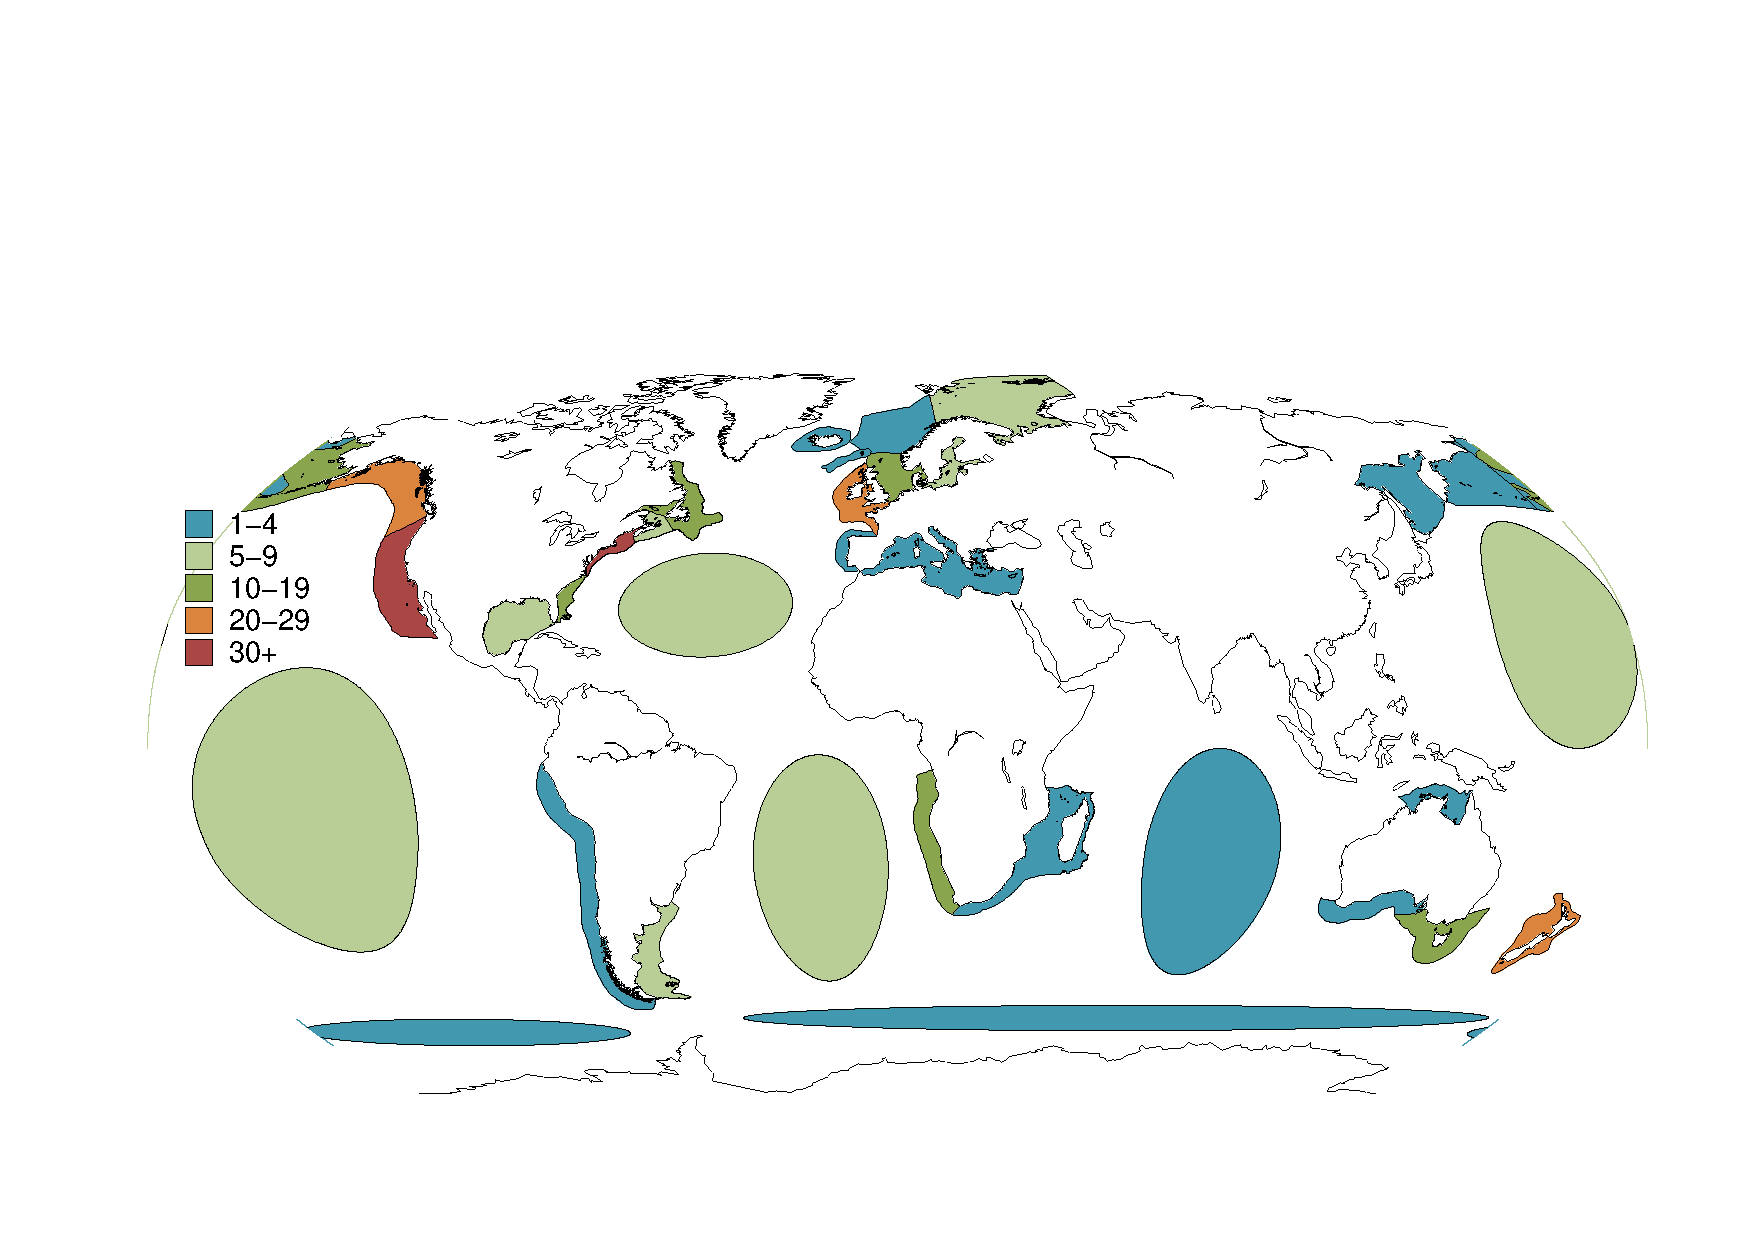
\includegraphics[width=15cm]{/home/srdbadmin/srdb/projects/fishandfisheries/GMT/stocks-byLME.pdf}
\end{center}
\caption{ }\label{fig:lmes}
\end{figure}

\begin{figure}
\begin{center}
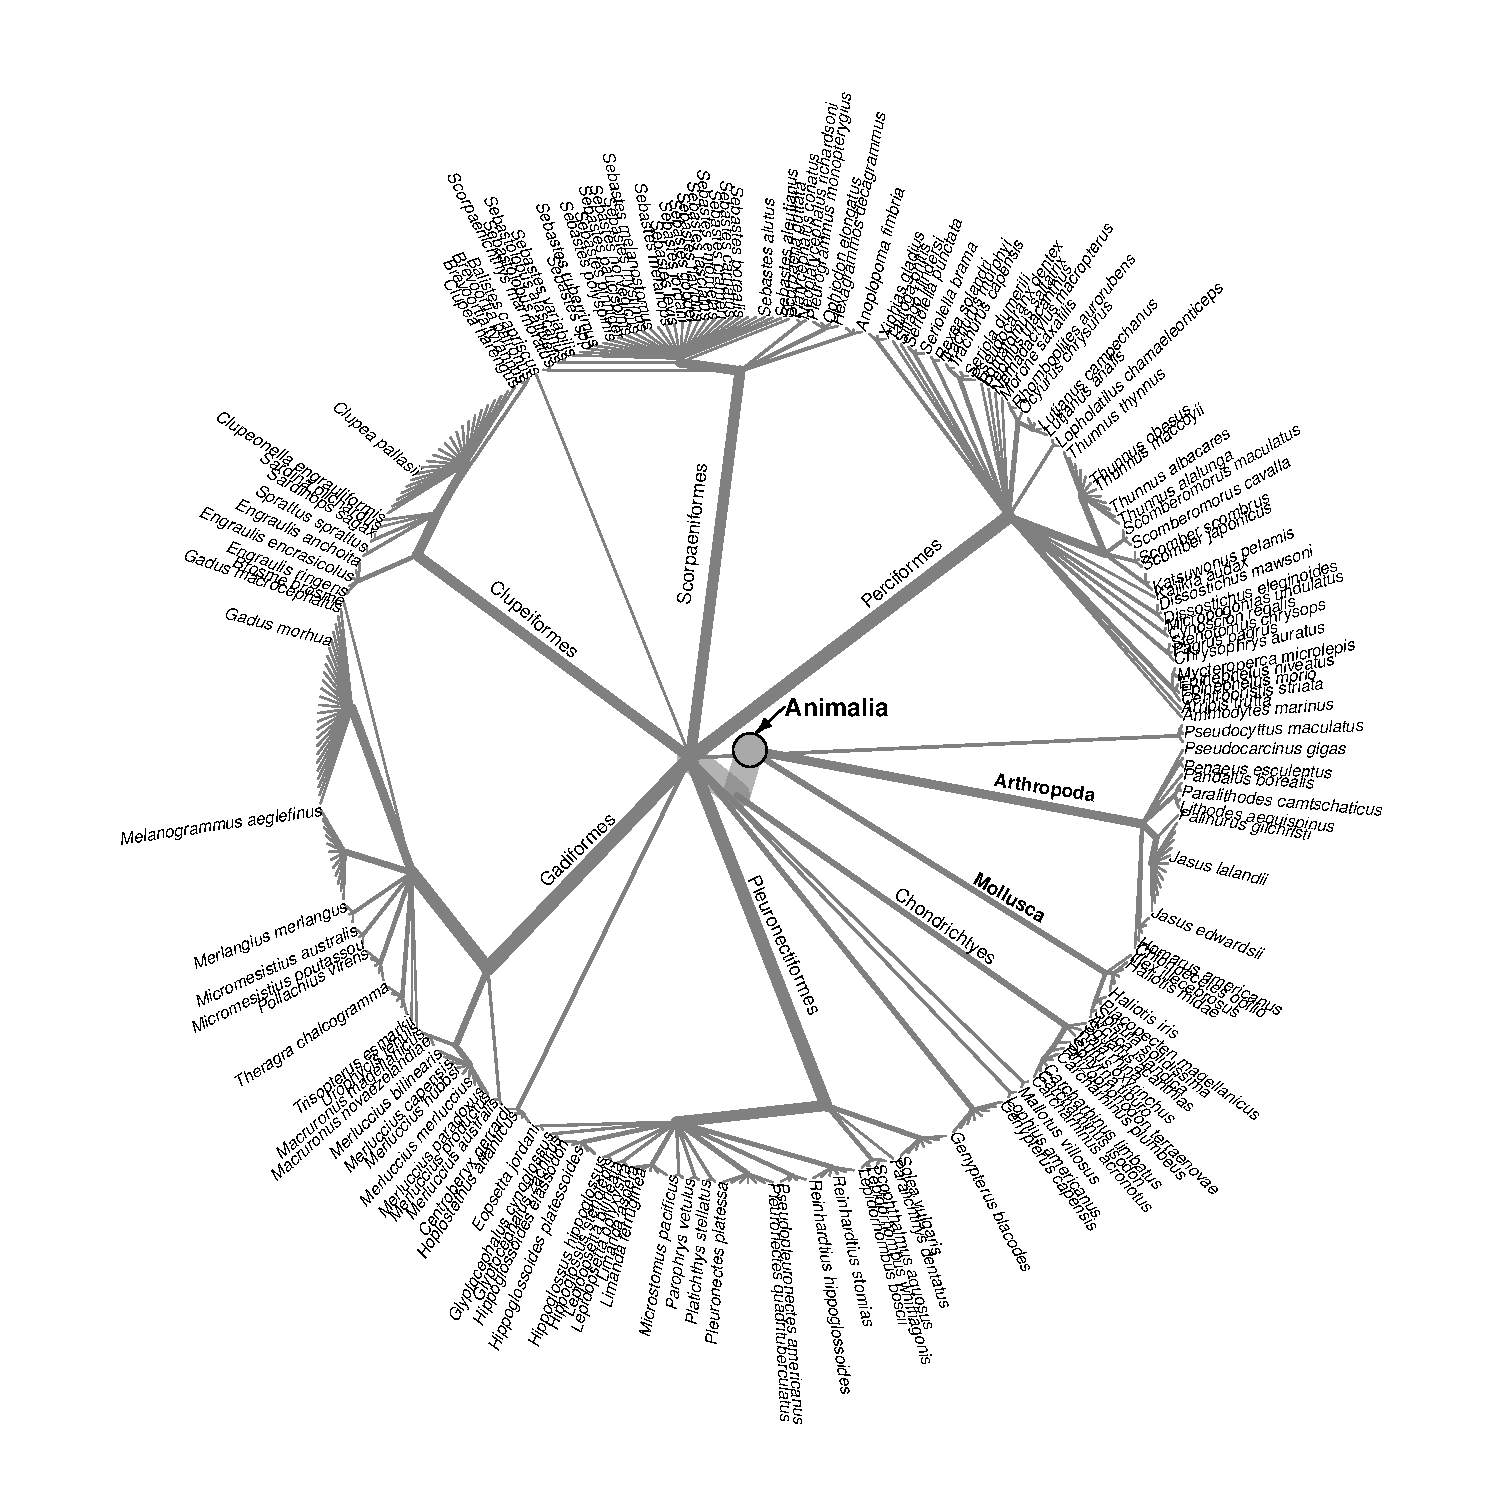
\includegraphics[width=15cm]{/home/srdbadmin/srdb/projects/fishandfisheries/R/srdb-by-assessment.pdf} %taxonomic_coverage_byLME.pdf}
\end{center}
\caption{ }\label{fig:taxo:srdb}
\end{figure}


\begin{figure}
\begin{center}
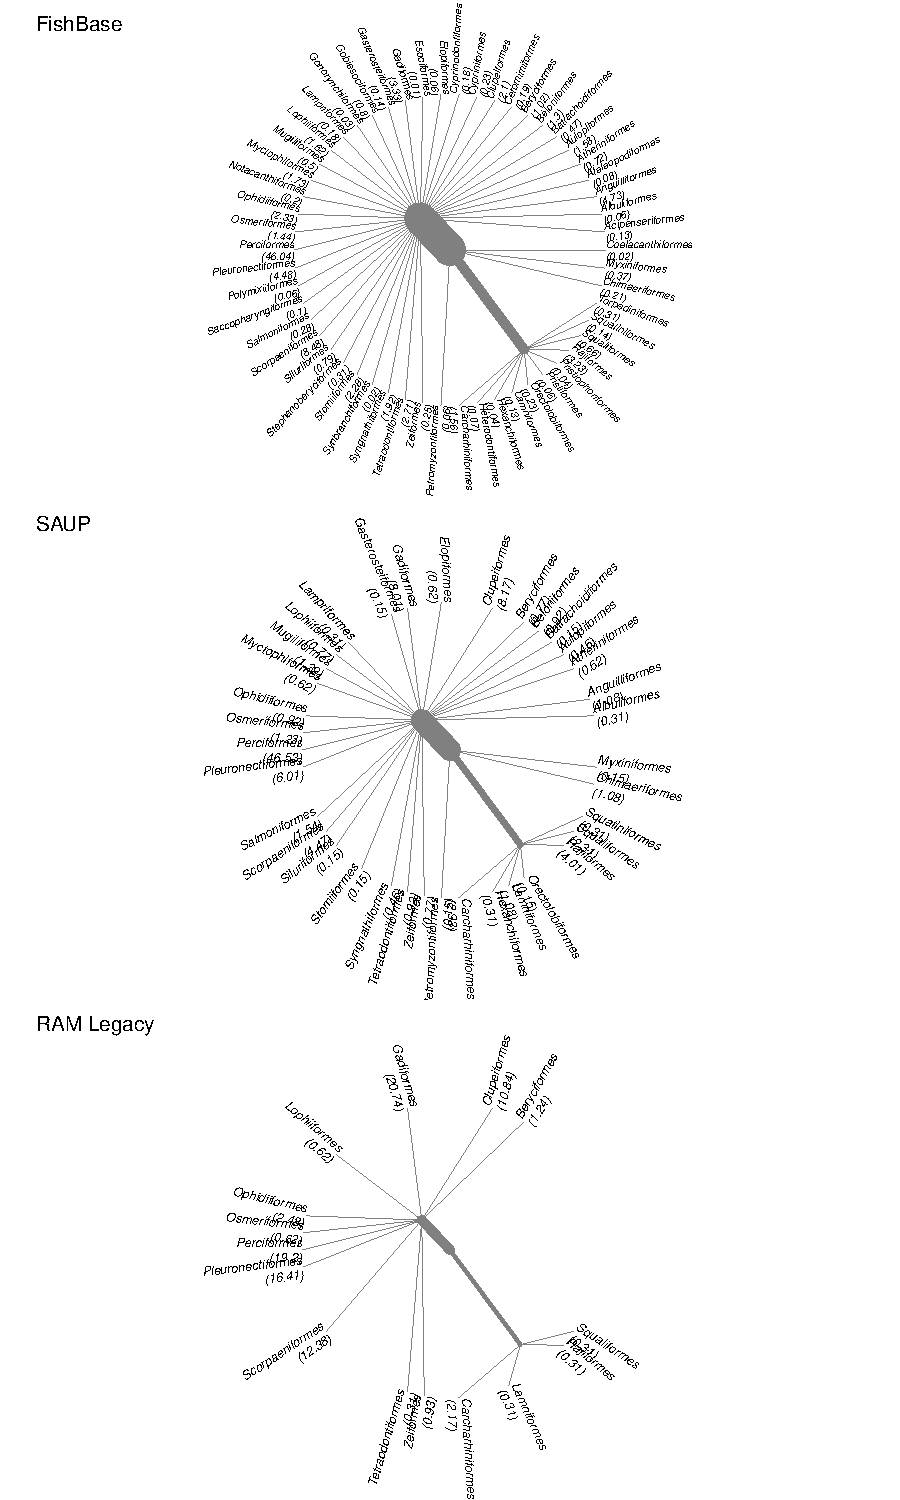
\includegraphics[width=12cm]{/home/srdbadmin/srdb/projects/fishandfisheries/R/three_panel_phylo.pdf} % fishbase_saup_two_panel_phylo.pdf}
\end{center}
\caption{ }\label{fig:taxo:threepanel}
\end{figure}

\begin{figure}
\begin{center}
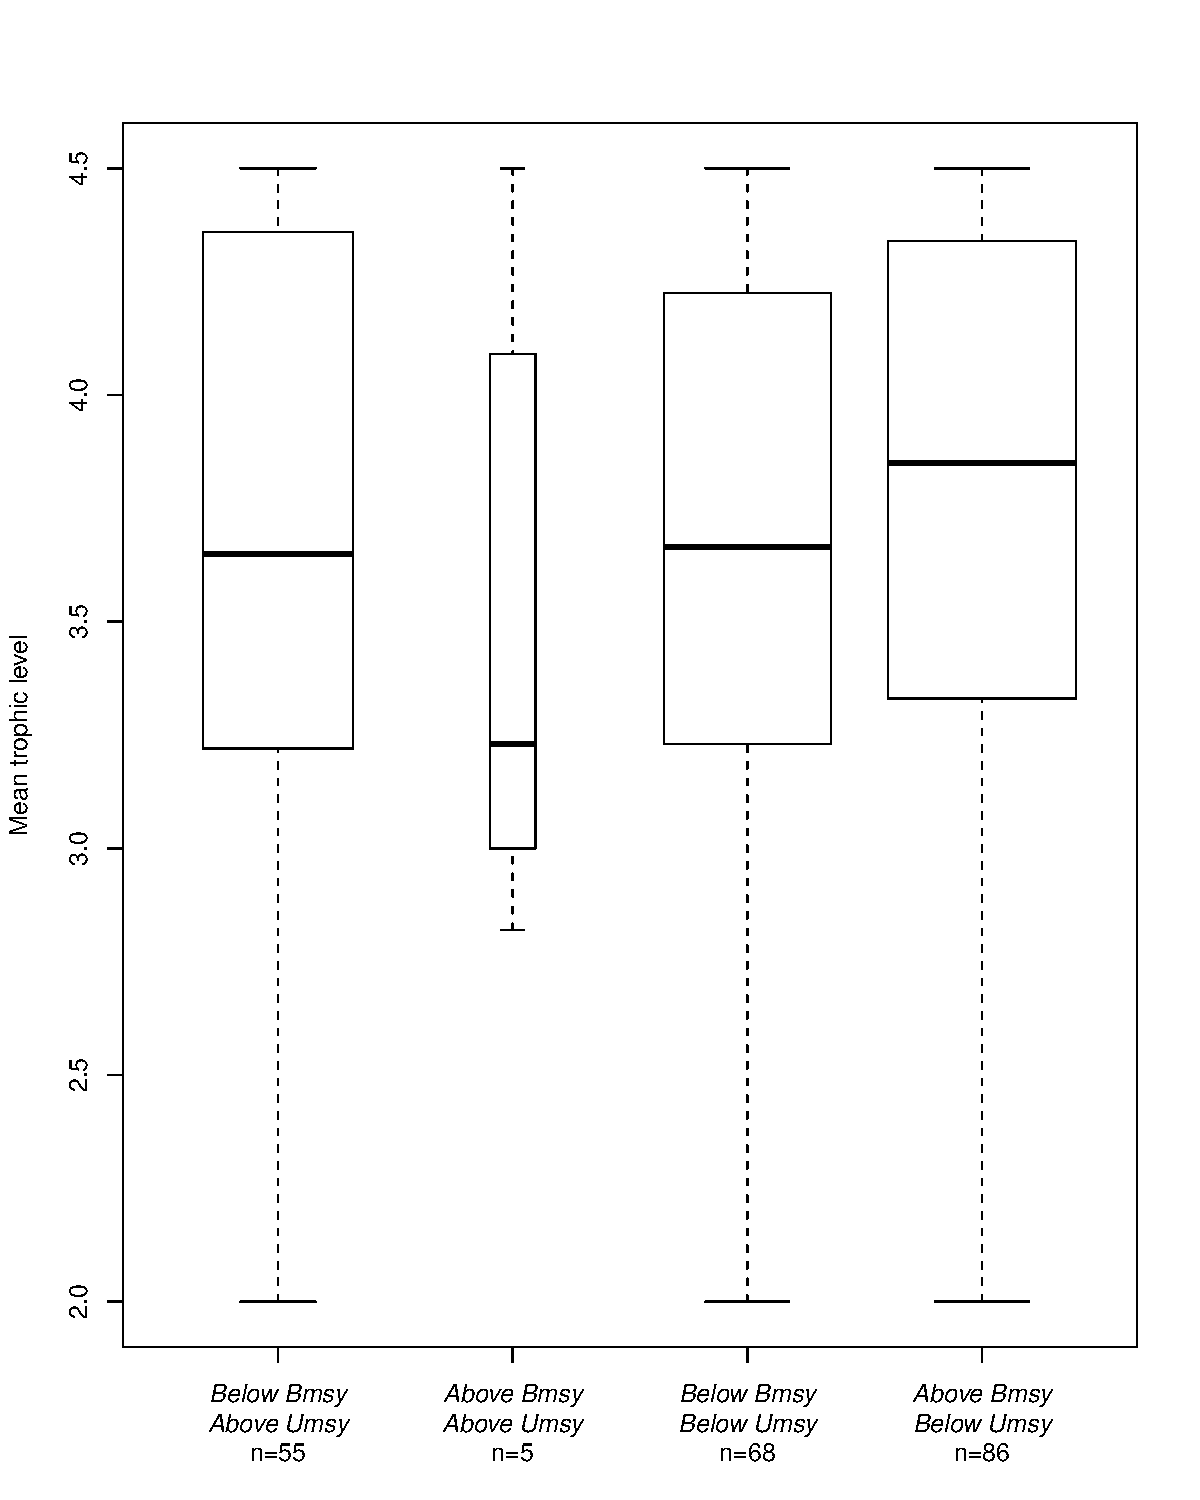
\includegraphics[width=15cm]{/home/srdbadmin/srdb/projects/fishandfisheries/R/TL-quadrant-srdb.pdf}
\end{center}
\caption{ }\label{fig:TL}
\end{figure}

\begin{figure}
\begin{center}
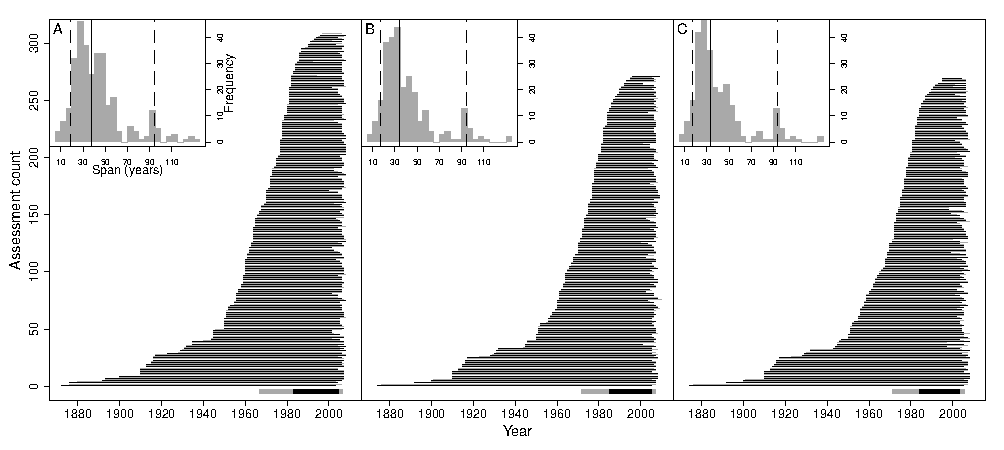
\includegraphics[width=15cm]{/home/srdbadmin/srdb/projects/fishandfisheries/R/orca_plot_v2.pdf}
\end{center}
\caption{ }\label{fig:orca}
\end{figure}

\begin{figure}
\begin{center}
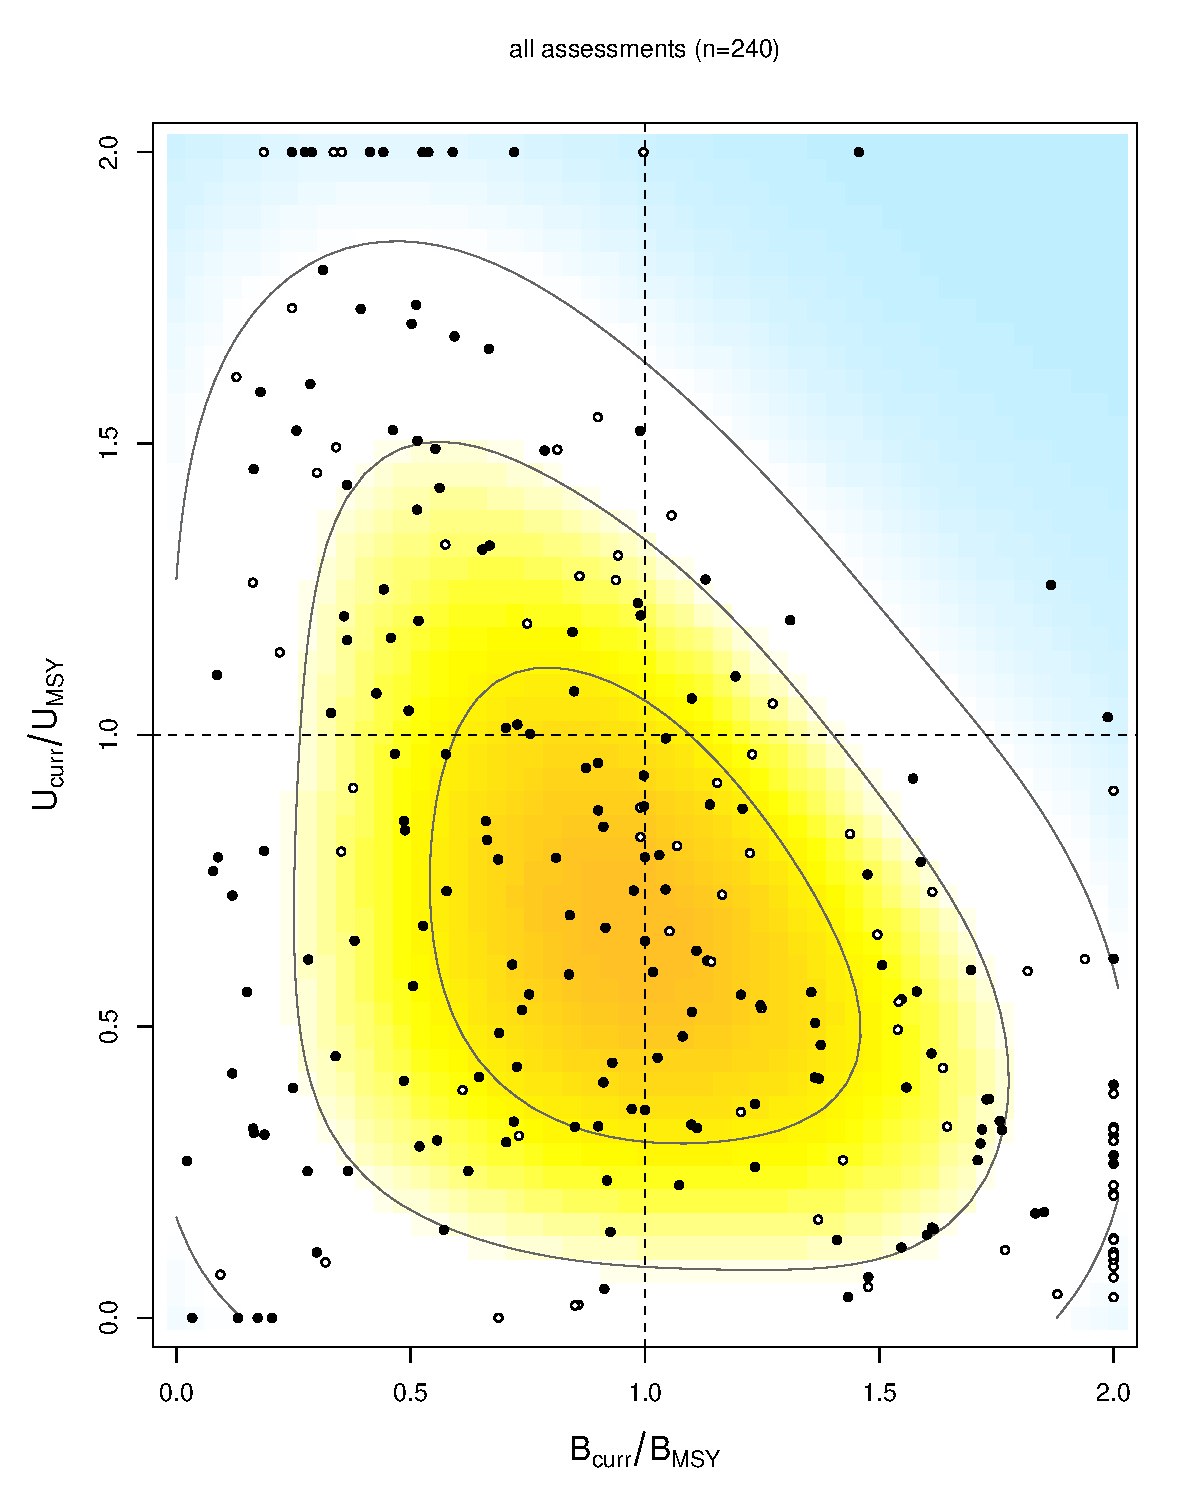
\includegraphics[width=15cm]{/home/srdbadmin/srdb/projects/fishandfisheries/R/friedegg-single.pdf}
\end{center}
\caption{ }\label{fig:friedegg}
\end{figure}

\begin{figure}
\begin{center}
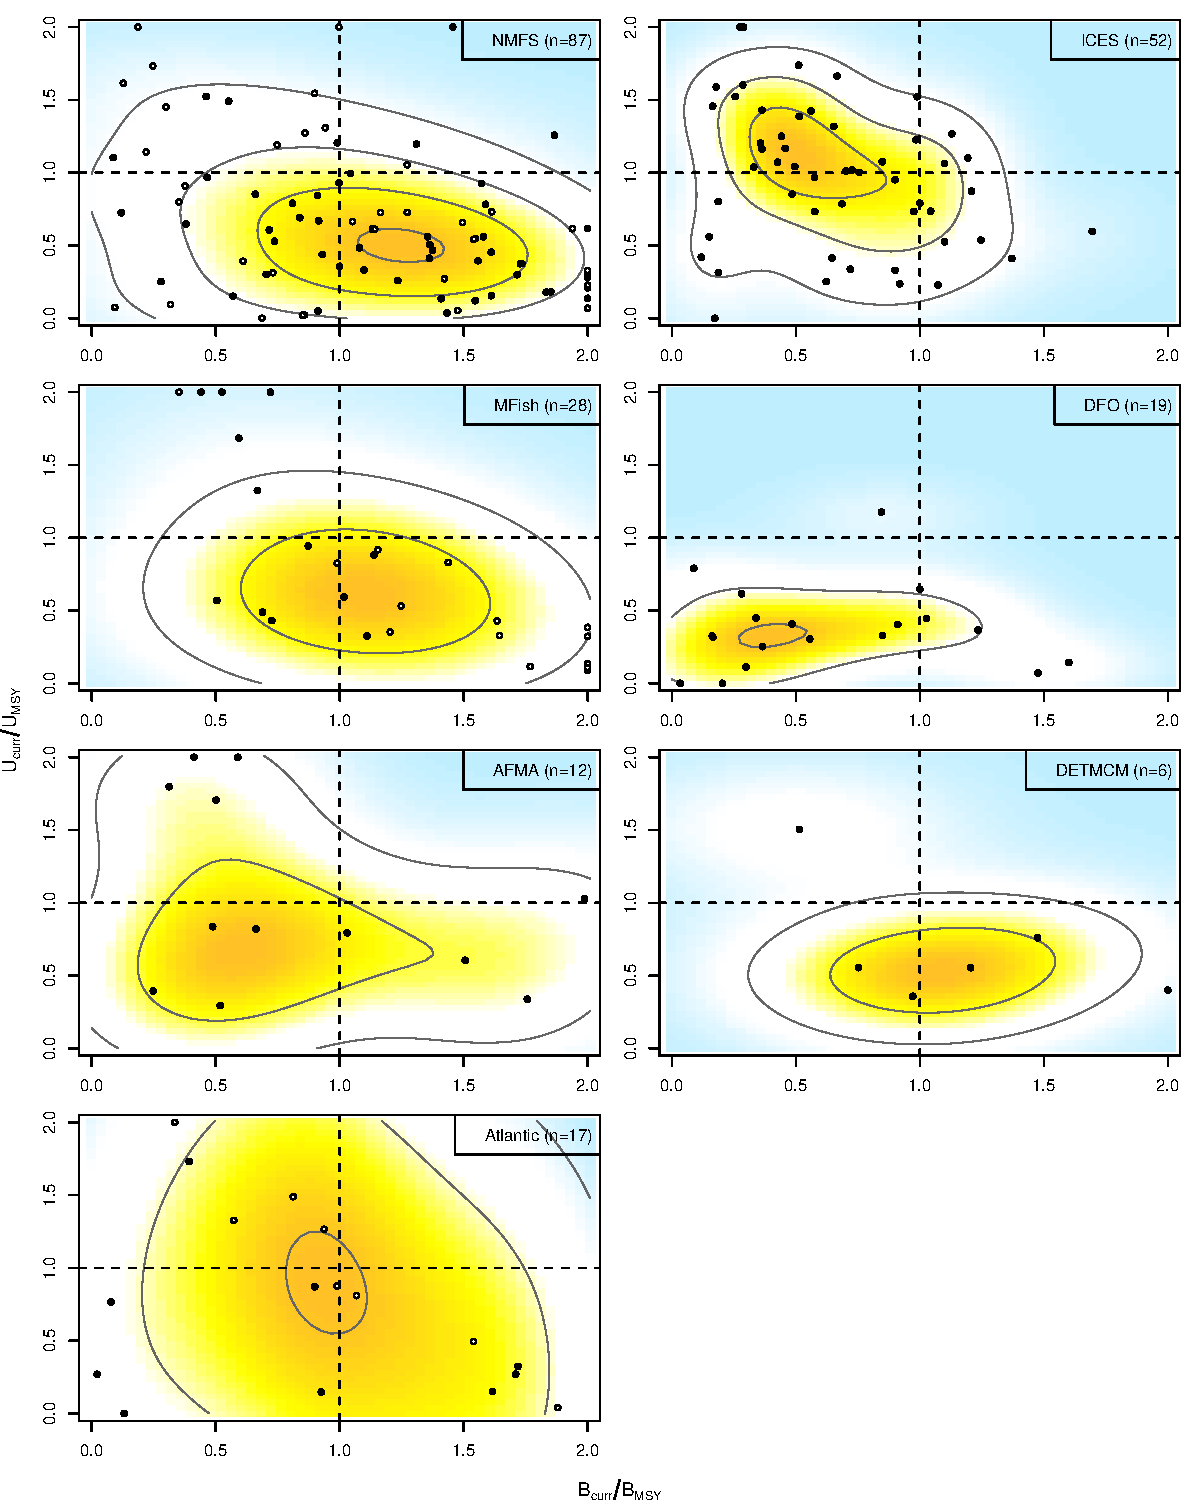
\includegraphics[width=15cm]{/home/srdbadmin/srdb/projects/fishandfisheries/R/friedegg-by-mgmt.pdf}
\end{center}
\caption{ }\label{fig:friedeggmgmt}
\end{figure}


%\appendix
%\section*{Supporting Information}

%\subsection*{Entity relationship diagram}
%\begin{figure}
%\begin{center}
%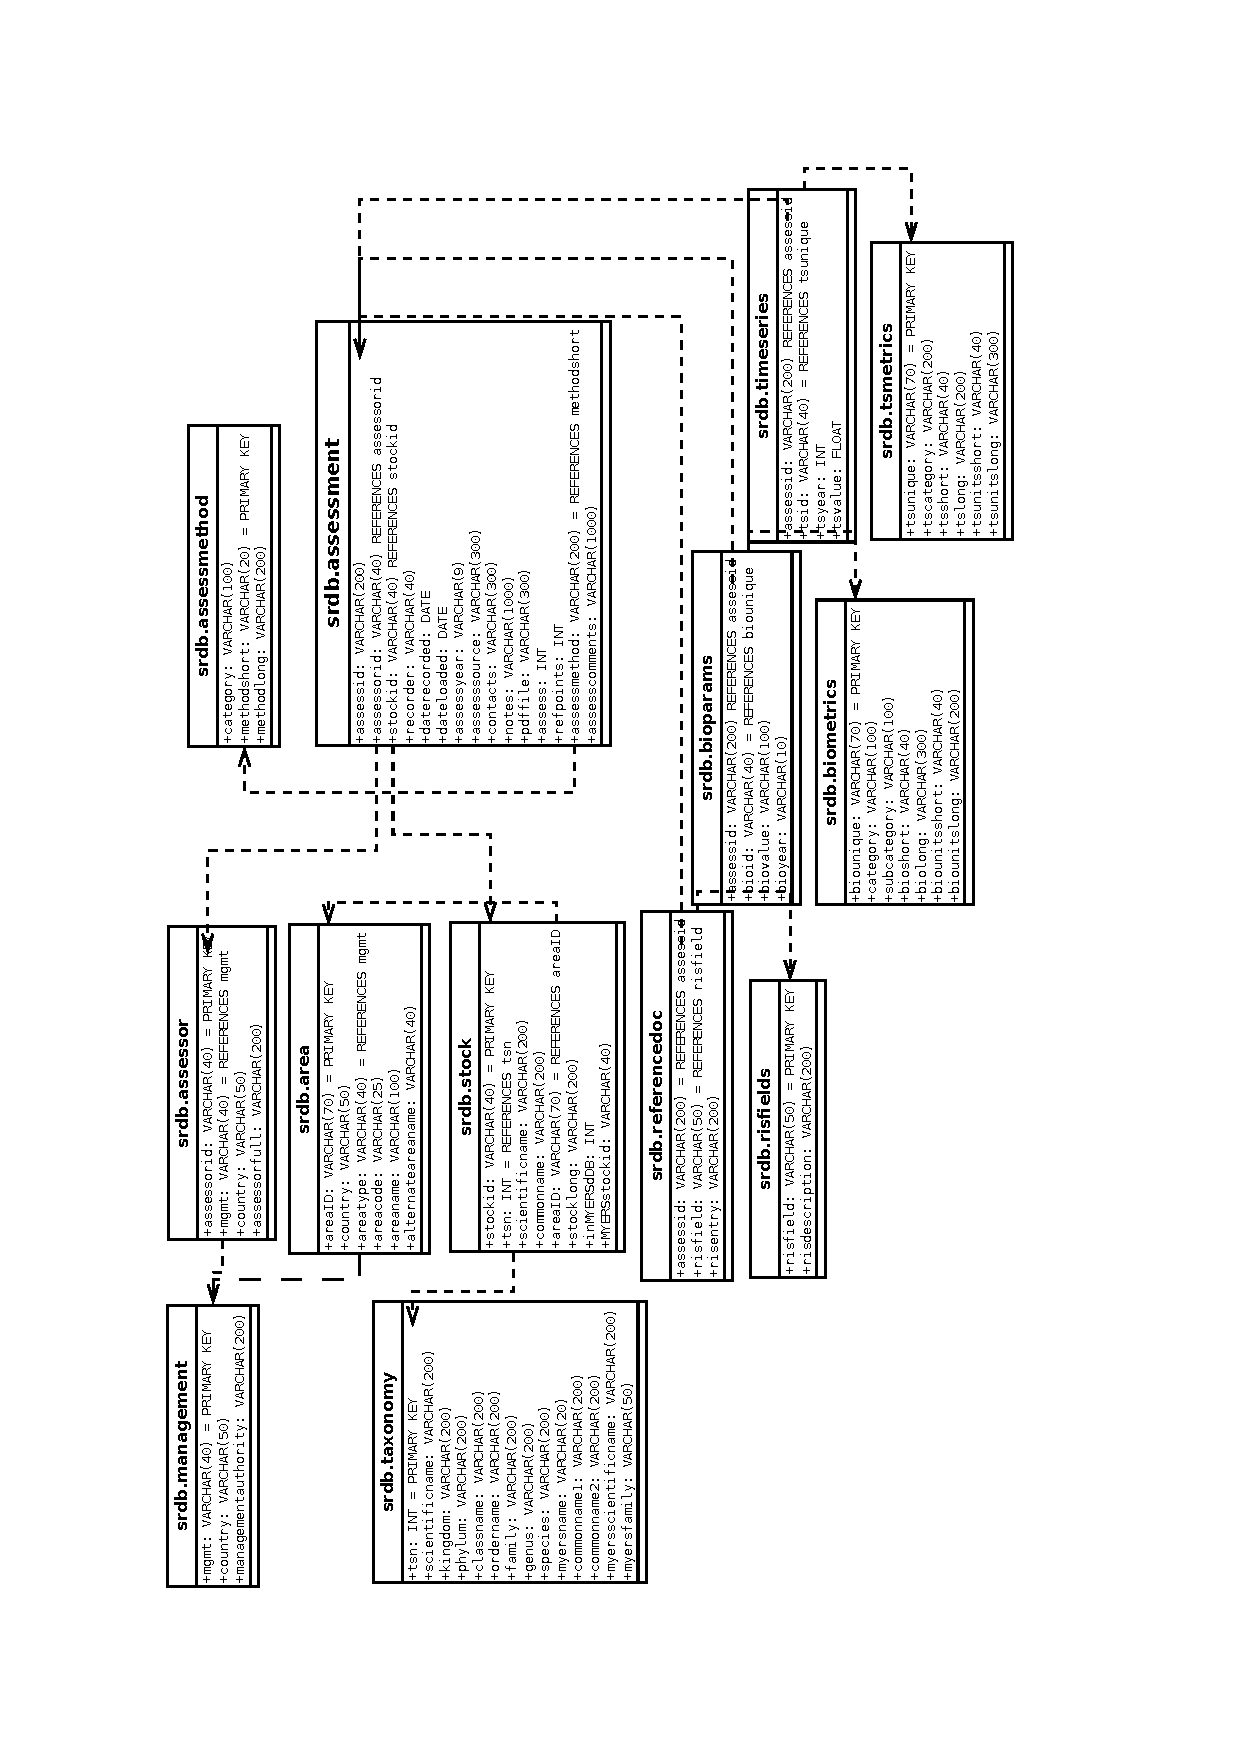
\includegraphics[width=15cm]{/home/srdbadmin/SQLpg/srdb/trunk/doc/srdb-ERD.pdf}
%\end{center}
%\caption{Entity relationship diagram of the RAM legacy database.}\label{fig:ERD}
%\end{figure}

%%% latex table generated in R 2.9.1 by xtable 1.5-6 package
% Wed Jul 28 15:08:19 2010
\begin{longtable}{p{1.8cm}p{3.5cm}p{3.5cm}p{3cm}cccp{0.9cm}cp{0.9cm}c}
  \hline
mgmt & stock & scientificname & assessmethod & timespan & currentyear & Bratio & bfromassessment & Uratio & ufromassessment & ref \\ 
  \hline
AFMA & Bight redfish Southeast Australia & \textit{Centroberyx gerrardi} & Integrated Analysis & 1958-2007 &  &  &  &  &  & \cite{BIGHTREDDEEPFLATSE.pdf} \\ 
  AFMA & New Zealand ling Eastern half of Southeast Australia & \textit{Genypterus blacodes} & Integrated Analysis & 1968-2007 & 2007 & 0.59 & yes & 2.20 & no & \cite{NZLINGSE.pdf} \\ 
  AFMA & New Zealand ling Western half of Southeast Australia & \textit{Genypterus blacodes} & Integrated Analysis & 1968-2007 &  &  &  &  &  & \cite{NZLINGSE.pdf} \\ 
  AFMA & Orange roughy Cascade Plateau & \textit{Hoplostethus atlanticus} & Integrated Analysis & 1987-2006 & 2006 & 1.76 & no & 0.34 & no & \cite{CSIRO-Cascade-Plateau-Stock-Assessment-2006.pdf} \\ 
  AFMA & Orange roughy Southeast Australia & \textit{Hoplostethus atlanticus} & Integrated Analysis & 1978-2007 & 2007 & 0.52 & yes & 0.29 & no & \cite{OROUGHYSE.pdf} \\ 
  AFMA & Jackass morwong Southeast Australia & \textit{Nemadactylus macropterus} & Integrated Analysis & 1913-2007 & 2007 & 0.31 & yes & 1.80 & no & \cite{MORWONGSE.pdf} \\ 
  AFMA & Tiger flathead Southeast Australia & \textit{Neoplatycephalus richardsoni} & Integrated Analysis & 1913-2006 & 2006 & 1.99 & yes & 1.03 & no & \cite{TIGERFLATSE.pdf} \\ 
  AFMA & Northern Australia brown tiger shrimp & \textit{Penaeus esculentus} & Biomass dynamics model & 1970-2006 &  &  &  &  &  & \cite{NORTHPRAWNS.pdf} \\ 
  AFMA & Northern Australia grooved Tiger Prawn & \textit{Penaeus esculentus} & Biomass dynamics model & 1970-2006 &  &  &  &  &  & \cite{NORTHPRAWNS.pdf} \\ 
  AFMA & Deepwater flathead Southeast Australia & \textit{Platycephalus conatus} & Integrated Analysis & 1978-2007 & 2007 & 1.51 & yes & 0.61 & no & \cite{BIGHTREDDEEPFLATSE.pdf} \\ 
  AFMA & Tasmanian giant crab Tasmania & \textit{Pseudocarcinus gigas} & Unknown & 1990-2007 & 2007 & 0.50 & no & 1.71 & no & \cite{JENSEN_TASGIANTCRAB_2008.pdf} \\ 
  AFMA & common gemfish Southeast Australia & \textit{Rexea solandri} & Integrated Analysis & 1966-2007 & 2007 & 0.25 & yes & 0.39 & no & \cite{GEMFISHSE.pdf} \\ 
  AFMA & Blue Warehou Eastern half of Southeast Australia & \textit{Seriolella brama} & Integrated Analysis & 1984-2006 & 2006 & 0.49 & yes & 0.84 & no & \cite{WAREHOUSE.pdf} \\ 
  AFMA & Blue Warehou Western half of Southeast Australia & \textit{Seriolella brama} & Integrated Analysis & 1984-2006 & 2006 & 0.41 & yes & 2.04 & no & \cite{WAREHOUSE.pdf} \\ 
  AFMA & Silverfish Southeast Australia & \textit{Seriolella punctata} & Integrated Analysis & 1978-2006 & 2006 & 1.03 & yes & 0.79 & no & \cite{SILVERFISHSE.pdf} \\ 
  AFMA & School whiting Southeast Australia & \textit{Sillago flindersi} & Integrated Analysis & 1945-2007 & 2007 & 0.66 & yes & 0.82 & no & \cite{SWHITSE.pdf} \\ 
  CCAMLR & Antarctic toothfish Ross Sea & \textit{Dissostichus mawsoni} & Integrated Analysis & 1995-2007 & 2007 & 1.76 & no & 0.32 & yes & \cite{ATOOTHFISHRS.pdf} \\ 
  CFP & Argentine anchoita Northern Argentina & \textit{Engraulis anchoita} & VPA & 1989-2007 & 2007 & 1.37 & yes & 0.17 & yes & \cite{Hansen-ANCHOVY-N-2007.pdf} \\ 
  CFP & Argentine anchoita Southern Argentina & \textit{Engraulis anchoita} & Biomass dynamics model & 1992-2007 & 2007 & 3.13 & yes & 0.04 & yes & \cite{Hansen-ANCHOVY-S-2007.pdf} \\ 
  CFP & Patagonian grenadier Southern Argentina & \textit{Macruronus magellanicus} & VPA & 1983-2006 & 2006 & 1.82 & yes & 0.60 & yes & \cite{Giussi-hoki-2007.pdf} \\ 
  CFP & Argentine hake Northern Argentina & \textit{Merluccius hubbsi} & VPA & 1985-2007 & 2007 & 0.16 & yes & 1.26 & yes & \cite{Irusta-hake-N-2007.pdf} \\ 
  CFP & Argentine hake Southern Argentina & \textit{Merluccius hubbsi} & VPA & 1985-2008 & 2008 & 0.34 & yes & 1.49 & yes & \cite{Renzi-hake-S-2009.pdf} \\ 
  CFP &  Southern blue whiting Southern Argentina & \textit{Micromesistius australis} & VPA & 1985-2007 &  &  &  &  &  & \cite{Giussi-polaca-2007.pdf} \\ 
  DETMCM & Patagonian toothfish South Africa Subantarctic Prince Edward Islands & \textit{Dissostichus eleginoides} & Biomass dynamics model & 1960-2008 &  &  &  &  &  & \cite{Branch-SA-Toothfish-2007.pdf} \\ 
  DETMCM & Anchovy South Africa & \textit{Engraulis encrasicolus} & Statistical catch at age model & 1984-2006 & 2006 & 0.97 & no & 0.36 & no & \cite{ANCHOSA.pdf} \\ 
  DETMCM & Kingklip South Africa & \textit{Genypterus capensis} & Biomass dynamics model & 1932-2008 & 2008 & 1.20 & yes & 0.55 & no & \cite{Branch-SA-Kingklip-2008.pdf} \\ 
  DETMCM & South African abalone South Africa & \textit{Haliotis midae} & Statistical catch at age model & 1951-2008 &  &  &  &  &  & \cite{Plaganyi-SA-abalone-2008NOVSWG-AB21.pdf} \\ 
  DETMCM & South African west coast rock lobster South Africa Areas 1-2 & \textit{Jasus lalandii} & Statistical catch at age model & 1910-2008 &  &  &  &  &  & \cite{Johnston-SAWestRockLobster-2007.pdf} \\ 
  DETMCM & South African west coast rock lobster South Africa Areas 3-4 & \textit{Jasus lalandii} & Statistical catch at age model & 1910-2008 &  &  &  &  &  & \cite{Johnston-SAWestRockLobster-2007.pdf} \\ 
  DETMCM & South African west coast rock lobster South Africa Areas 5-6 & \textit{Jasus lalandii} & Statistical catch at age model & 1910-2008 &  &  &  &  &  & \cite{Johnston-SAWestRockLobster-2007.pdf} \\ 
  DETMCM & South African west coast rock lobster South Africa Area 7 & \textit{Jasus lalandii} & Statistical catch at age model & 1910-2008 &  &  &  &  &  & \cite{Johnston-SAWestRockLobster-2007.pdf} \\ 
  DETMCM & South African west coast rock lobster South Africa Area 8 & \textit{Jasus lalandii} & Statistical catch at age model & 1910-2008 &  &  &  &  &  & \cite{Johnston-SAWestRockLobster-2007.pdf} \\ 
  DETMCM & Shallow-water cape hake South Africa & \textit{Merluccius capensis} & Biomass dynamics model & 1917-2008 & 2008 & 2.30 & yes & 0.40 & no & \cite{SA-Mparadoxus-2008-IWS-DEC08-H-5.pdf} \\ 
  DETMCM & Deep-water cape hake South Africa & \textit{Merluccius paradoxus} & Biomass dynamics model & 1917-2008 &  &  &  &  &  & \cite{SA-Mparadoxus-2008-IWS-DEC08-H-5.pdf} \\ 
  DETMCM & Southern spiny lobster South Africa South coast & \textit{Palinurus gilchristi} & Statistical catch at age model & 1973-2008 & 2008 & 0.51 & no & 1.50 & no & \cite{Johnston-SASouthRockLobster-2008.pdf} \\ 
  DETMCM & Sardine South Africa & \textit{Sardinops sagax} & Statistical catch at age model & 1984-2006 & 2006 & 0.75 & no & 0.55 & no & \cite{deMoorSASardineAssessment-Sep07.pdf} \\ 
  DETMCM & Cape horse mackerel South Africa South coast & \textit{Trachurus capensis} & Biomass dynamics model & 1950-2007 & 2007 & 1.47 & no & 0.76 & no & \cite{Johnston-SAHorseMackerel-2007.pdf} \\ 
  DFO & Herring Scotian Shelf and Bay of Fundy & \textit{Clupea harengus} & VPA & 1965-2006 &  &  &  &  &  & \cite{NAFO-HERR4VWX-2006.pdf} \\ 
  DFO & Herring NAFO 4R fall spawners & \textit{Clupea harengus} & VPA & 1971-2003 &  &  &  &  &  & \cite{NAFO-HERR4RSP-2004.pdf} \\ 
  DFO & Herring NAFO 4R spring spawners & \textit{Clupea harengus} & VPA & 1963-2004 &  &  &  &  &  & \cite{NAFO-HERR4RSP-2004.pdf} \\ 
  DFO & Herring NAFO 4T fall spawners & \textit{Clupea harengus} & VPA & 1974-2007 &  &  &  &  &  & \cite{NAFO-HERR4TFA-2007.pdf} \\ 
  DFO & Herring NAFO 4T spring spawners & \textit{Clupea harengus} & VPA & 1974-2007 &  &  &  &  &  & \cite{NAFO-HERR4TFA-2007.pdf} \\ 
  DFO & Pacific herring Central Coast & \textit{Clupea pallasii} & Statistical catch at age model & 1951-2007 & 2007 & 0.30 & no & 0.11 & no & \cite{RES2007_002_e.pdf} \\ 
  DFO & Pacific herring Prince Rupert District & \textit{Clupea pallasii} & Statistical catch at age model & 1951-2007 & 2007 & 0.16 & no & 0.32 & no & \cite{RES2007_002_e.pdf} \\ 
  DFO & Pacific herring Queen Charlotte Islands & \textit{Clupea pallasii} & Statistical catch at age model & 1951-2007 & 2007 & 0.20 & no & 0.00 & no & \cite{RES2007_002_e.pdf} \\ 
  DFO & Pacific herring Straight of Georgia & \textit{Clupea pallasii} & Statistical catch at age model & 1951-2007 & 2007 & 0.91 & no & 0.40 & no & \cite{RES2007_002_e.pdf} \\ 
  DFO & Pacific herring West Coast of Vancouver Island & \textit{Clupea pallasii} & Statistical catch at age model & 1951-2007 & 2007 & 0.03 & no & 0.00 & no & \cite{RES2007_002_e.pdf} \\ 
  DFO & Pacific cod Hecate Strait & \textit{Gadus macrocephalus} & Biomass dynamics model & 1956-2005 & 2004 & 0.37 & no & 0.25 & no & \cite{RES2005_026_Cod.pdf} \\ 
  DFO & Pacific cod West Coast of Vancouver Island & \textit{Gadus macrocephalus} & Biomass dynamics model & 1956-2002 & 2001 & 0.28 & no & 0.61 & no & \cite{ref2002-113.pdf} \\ 
  DFO & Atlantic cod NAFO 5Zjm & \textit{Gadus morhua} & VPA & 1978-2003 & 2002 & 0.34 & no & 0.45 & no & \cite{NAFO-COD5Zjm-2003.pdf} \\ 
  DFO & Atlantic cod NAFO 2J3KL inshore & \textit{Gadus morhua} & VPA & 1959-2006 & 2005 & 1.60 & no & 0.14 & no & \cite{DFO-COD2J3KLIS-2006.pdf} \\ 
  DFO & Atlantic cod NAFO 3Ps & \textit{Gadus morhua} & VPA & 1959-2004 & 2004 & 0.49 & no & 0.41 & no & \cite{DFO-COD3Ps-2004.pdf} \\ 
  DFO & Atlantic cod NAFO 3Pn4RS & \textit{Gadus morhua} & VPA & 1964-2007 & 2006 & 0.09 & no & 0.79 & no & \cite{DFO-COD3Pn4Rs-2007.pdf} \\ 
  DFO & Atlantic cod NAFO 4TVn & \textit{Gadus morhua} & VPA & 1965-2007 & 2006 & 0.17 & no & 0.32 & no & \cite{NAFO-COD4TVn-2007.pdf} \\ 
  DFO & Rock sole Hecate Strait & \textit{Lepidopsetta bilineata} & Statistical catch at age model & 1945-2001 & 2001 & 1.03 & no & 0.45 & no & \cite{Flat99.pdf} \\ 
  DFO & Haddock NAFO-4X5Y & \textit{Melanogrammus aeglefinus} & VPA & 1960-2003 & 2003 & 0.85 & no & 0.33 & no & \cite{NAFO-HAD4X5Y-2003.pdf} \\ 
  DFO & Haddock NAFO-5Zejm & \textit{Melanogrammus aeglefinus} & VPA & 1968-2003 & 2002 & 1.00 & no & 0.65 & no & \cite{NAFO-HAD5Zejm-2003.pdf} \\ 
  DFO & English sole Hecate Strait & \textit{Parophrys vetulus} & Statistical catch at age model & 1944-2001 & 2001 & 1.23 & no & 0.37 & no & \cite{Flat99.pdf} \\ 
  DFO & Pollock NAFO-4VWX5Zc & \textit{Pollachius virens} & VPA & 1974-2007 & 2006 & 0.56 & no & 0.30 & no & \cite{NAFO-POLL4VWX5Zc-2006.pdf} \\ 
  IATTC & Yellowfin tuna Eastern Pacific & \textit{Thunnus albacares} & Statistical catch at age model & 1975-2007 &  &  &  &  &  & \cite{SAR8-YFT-ENG.pdf} \\ 
  IATTC & Bigeye tuna Eastern Pacific & \textit{Thunnus obesus} & Integrated Analysis & 1975-2007 &  &  &  &  &  & \cite{JENSEN_BETEPAC_2008.pdf} \\ 
  ICCAT & Skipjack tuna Eastern Atlantic & \textit{Katsuwonus pelamis} & Biomass dynamics model & 1950-2006 & 2006 & 1.71 & no & 0.27 & yes & \cite{JENSEN-YFINATL-2008.pdf} \\ 
  ICCAT & Skipjack tuna Western Atlantic & \textit{Katsuwonus pelamis} & Biomass dynamics model & 1952-2006 & 2006 & 1.72 & no & 0.32 & yes & \cite{JENSEN-YFINATL-2008.pdf} \\ 
  ICCAT & Albacore tuna North Atlantic & \textit{Thunnus alalunga} & VPA & 1929-2005 & 2005 & 0.81 & yes & 1.49 & yes & \cite{ref2007-ALB-STOCK-ASSESS-REP.pdf} \\ 
  ICCAT & Yellowfin tuna Atlantic & \textit{Thunnus albacares} & VPA & 1970-2006 & 2006 & 1.07 & yes & 0.81 & yes & \cite{JENSEN-YFINATL-2008.pdf} \\ 
  ICCAT & Bigeye tuna Atlantic & \textit{Thunnus obesus} & Biomass dynamics model & 1950-2005 & 2005 & 0.90 & no & 0.87 & yes & \cite{JENSEN-BIGEYEATL-2008.pdf} \\ 
  ICCAT & Bluefin tuna Eastern Atlantic & \textit{Thunnus thynnus} & VPA & 1969-2007 & 2007 & 0.34 & yes & 9.38 & yes & \cite{ref2008-BFT-STOCK-ASSESS-REP.pdf} \\ 
  ICCAT & Bluefin tuna Western Atlantic & \textit{Thunnus thynnus} & VPA & 1969-2007 & 2007 & 0.57 & yes & 1.33 & yes & \cite{ref2008-BFT-STOCK-ASSESS-REP.pdf} \\ 
  ICCAT & Swordfish Mediterranean Sea & \textit{Xiphias gladius} & Biomass dynamics model & 1968-2006 & 2006 & 0.94 & yes & 1.27 & yes & \cite{ICCAT-Mediterranean-Xiphiasgladius-2007.pdf} \\ 
  ICCAT & Swordfish North Atlantic & \textit{Xiphias gladius} & Biomass dynamics model & 1978-2007 & 2005 & 0.99 & yes & 0.88 & yes & \cite{JENSEN-SWORDSATL-2007.pdf} \\ 
  ICCAT & Swordfish South Atlantic & \textit{Xiphias gladius} & Biomass dynamics model & 1970-2005 & 2005 & 1.54 & yes & 0.49 & yes & \cite{JENSEN-SWORDSATL-2007.pdf} \\ 
  ICES & Sandeel North Sea & \textit{Ammodytes marinus} & VPA & 1983-2007 & 2007 & 0.92 & no & 0.24 & no & \cite{ICES-WGNSSK-2007.pdf} \\ 
  ICES & Herring ICES 22-24-IIIa & \textit{Clupea harengus} & Statistical catch at age model & 1991-2006 & 2006 & 0.73 & no & 1.02 & no & \cite{ICES-HAWG-2007.pdf} \\ 
  ICES & Herring Northern Irish Sea & \textit{Clupea harengus} & Statistical catch at age model & 1960-2006 & 2006 & 0.72 & no & 0.34 & no & \cite{ICES-HAWG-2007.pdf} \\ 
  ICES & Herring North Sea & \textit{Clupea harengus} & Statistical catch at age model & 1960-2007 & 2006 & 0.65 & no & 1.32 & no & \cite{ICES-HAWG-2007.pdf} \\ 
  ICES & Herring ICES VIa & \textit{Clupea harengus} & Statistical catch at age model & 1957-2006 & 2006 & 0.18 & no & 1.59 & no & \cite{ICES-HAWG-2007.pdf} \\ 
  ICES & Herring ICES VIa-VIIb-VIIc & \textit{Clupea harengus} & VPA & 1969-2000 & 2000 & 0.50 & no & 1.04 & no & \cite{ICES-HAWG-2007.pdf} \\ 
  ICES & Herring ICES 25-32 & \textit{Clupea harengus} & VPA & 1973-2006 & 2006 & 0.69 & no & 0.79 & no & \cite{ICES-WGBFAS-2007.pdf} \\ 
  ICES & Herring ICES 30 & \textit{Clupea harengus} & VPA & 1972-2007 & 2006 & 1.19 & no & 1.10 & no & \cite{ICES-WGBFAS-2007.pdf} \\ 
  ICES & Herring ICES 31 & \textit{Clupea harengus} & VPA & 1979-2006 & 2006 & 0.29 & no & 1.60 & no & \cite{ICES-WGBFAS-2007.pdf} \\ 
  ICES & Herring Iceland (Summer spawners) & \textit{Clupea harengus} & VPA & 1983-2007 & 2006 & 1.00 & no & 0.79 & no & \cite{ICES-NWWG-2007.pdf} \\ 
  ICES & Herring ICES 28 & \textit{Clupea harengus} & VPA & 1976-2007 & 2006 & 1.21 & no & 0.87 & no & \cite{ICES-WGBFAS-2007.pdf} \\ 
  ICES & Anchovy ICES VIII & \textit{Engraulis encrasicolus} & Biomass dynamics model & 1986-2007 &  &  &  &  &  & \cite{ICES-WGMHSA007.pdf} \\ 
  ICES & Atlantic cod coastal Norway & \textit{Gadus morhua} & VPA & 1982-2006 & 2006 & 0.27 & no & 2.17 & no & \cite{ICES-AFWG-2007.pdf} \\ 
  ICES & Atlantic cod Northeast Arctic & \textit{Gadus morhua} & VPA & 1943-2006 & 2006 & 0.56 & no & 1.42 & no & \cite{ICES-AFWG-2007.pdf} \\ 
  ICES & Atlantic cod Faroe Plateau & \textit{Gadus morhua} & VPA & 1959-2006 & 2006 & 0.26 & no & 1.52 & no & \cite{ICES-NWWG-2007.pdf} \\ 
  ICES & Atlantic cod Iceland & \textit{Gadus morhua} & Statistical catch at age model & 1952-2006 & 2006 & 0.46 & no & 1.17 & no & \cite{ICES-NWWG-2007.pdf} \\ 
  ICES & Atlantic cod Baltic Areas 22 and 24 & \textit{Gadus morhua} & VPA & 1969-2007 & 2006 & 0.36 & no & 1.43 & no & \cite{ICES-WGBFAS-2007.pdf} \\ 
  ICES & Atlantic cod Baltic Areas 25-32 & \textit{Gadus morhua} & VPA & 1964-2007 & 2006 & 0.16 & no & 1.46 & no & \cite{ICES-WGBFAS-2007.pdf} \\ 
  ICES & Atlantic cod Kattegat & \textit{Gadus morhua} & VPA & 1970-2006 & 2006 & 0.19 & no & 0.31 & no & \cite{ICES-WGBFAS-2007.pdf} \\ 
  ICES & Atlantic cod Irish Sea & \textit{Gadus morhua} & VPA & 1968-2006 & 2006 & 0.15 & no & 0.56 & no & \cite{ICES-WGNSDS-2007.pdf} \\ 
  ICES & Atlantic cod West of Scotland & \textit{Gadus morhua} & Statistical catch at age model & 1977-2006 & 2006 & 0.12 & no & 0.42 & no & \cite{ICES-WGNSDS-2007.pdf} \\ 
  ICES & Atlantic cod North Sea & \textit{Gadus morhua} & VPA & 1962-2007 & 2006 & 0.19 & no & 0.80 & no & \cite{ICES-WGNSSK-2007.pdf} \\ 
  ICES & Fourspotted megrim ICES VIIIc-IXa & \textit{Lepidorhombus boscii} & VPA & 1986-2006 & 2006 & 0.70 & no & 1.01 & no & \cite{ICES-WGHMM-2007.pdf} \\ 
  ICES & Megrim ICES VIIIc-IXa & \textit{Lepidorhombus whiffiagonis} & VPA & 1985-2007 & 2006 & 0.43 & no & 1.07 & no & \cite{ICES-WGHMM-2007.pdf} \\ 
  ICES & Capelin Barents Sea & \textit{Mallotus villosus} & Unknown & 1965-2007 & 2006 & 0.17 & no & 0.00 & no & \cite{ICES-AFWG-2007.pdf} \\ 
  ICES & Capelin Iceland & \textit{Mallotus villosus} & Survey index & 1977-2007 & 2006 & 0.49 & no & 0.85 & no & \cite{ICES-NWWG-2007.pdf} \\ 
  ICES & Haddock Northeast Arctic & \textit{Melanogrammus aeglefinus} & VPA & 1947-2006 & 2006 & 1.10 & no & 1.06 & no & \cite{ICES-AFWG-2007.pdf} \\ 
  ICES & Haddock Faroe Plateau & \textit{Melanogrammus aeglefinus} & VPA & 1955-2006 & 2006 & 0.85 & no & 1.07 & no & \cite{ICES-NWWG-2007.pdf} \\ 
  ICES & Haddock Iceland & \textit{Melanogrammus aeglefinus} & VPA & 1977-2007 & 2007 & 0.98 & no & 1.23 & no & \cite{ICES-NWWG-2007.pdf} \\ 
  ICES & Haddock Irish Sea & \textit{Melanogrammus aeglefinus} & Survey index & 1972-2006 &  &  &  &  &  & \cite{ICES-WGNSDS-2007.pdf} \\ 
  ICES & Haddock West of Scotland & \textit{Melanogrammus aeglefinus} & Statistical catch at age model & 1977-2006 & 2006 & 0.58 & no & 0.73 & no & \cite{ICES-WGNSDS-2007.pdf} \\ 
  ICES & Haddock ICES IIIa and North Sea & \textit{Melanogrammus aeglefinus} & VPA & 1963-2006 & 2006 & 0.62 & no & 0.25 & no & \cite{ICES-WGNSSK-2007.pdf} \\ 
  ICES & Haddock Rockall Bank & \textit{Melanogrammus aeglefinus} & VPA & 1990-2007 & 2006 & 1.10 & no & 0.52 & no & \cite{ICES-WGNSDS-2007.pdf} \\ 
  ICES & Haddock ICES VIIb-k & \textit{Melanogrammus aeglefinus} & VPA & 1993-2006 & 2006 & 1.37 & no & 0.41 & no & \cite{ICES-WGSSDS-2007.pdf} \\ 
  ICES & Whiting ICES VIa & \textit{Merlangius merlangus} & Survey index & 1984-2007 &  &  &  &  &  & \cite{ICES-WGNSDS-2007.pdf} \\ 
  ICES & Whiting ICES IIIa, VIId and North Sea & \textit{Merlangius merlangus} & VPA & 1979-2006 & 2006 & 0.33 & no & 1.04 & no & \cite{ICES-WGNSSK-2007.pdf} \\ 
  ICES & Whiting ICES VIIe-k & \textit{Merlangius merlangus} & VPA & 1982-2007 & 2006 & 0.44 & no & 1.25 & no & \cite{ICES-WGSSDS-2007.pdf} \\ 
  ICES & Hake Northeast Atlantic North & \textit{Merluccius merluccius} & VPA & 1977-2007 & 2006 & 1.04 & no & 0.74 & no & \cite{ICES-WGHMM-2007.pdf} \\ 
  ICES & Hake Northeast Atlantic South & \textit{Merluccius merluccius} & VPA & 1982-2007 &  &  &  &  &  & \cite{ICES-WGHMM-2007.pdf} \\ 
  ICES & Whiting Northeast Atlantic & \textit{Micromesistius poutassou} & Integrated Analysis & 1980-2007 & 2006 & 0.67 & no & 1.66 & no & \cite{ICES-WGNPBW-2007.pdf} \\ 
  ICES & European Plaice Irish Sea & \textit{Pleuronectes platessa} & Statistical catch at age model & 1962-2006 & 2006 & 1.07 & no & 0.23 & no & \cite{ICES-WGNSDS-2007.pdf} \\ 
  ICES & European Plaice ICES VIId & \textit{Pleuronectes platessa} & VPA & 1979-2006 &  &  &  &  &  & \cite{ICES-WGNSSK-2007.pdf} \\ 
  ICES & European Plaice ICES IIIa & \textit{Pleuronectes platessa} & VPA & 1976-2006 &  &  &  &  &  & \cite{ICES-WGNSSK-2007.pdf} \\ 
  ICES & European Plaice North Sea & \textit{Pleuronectes platessa} & VPA & 1956-2006 &  &  &  &  &  & \cite{ICES-WGNSSK-2007.pdf} \\ 
  ICES & European Plaice ICES VIIf-g & \textit{Pleuronectes platessa} & VPA & 1976-2006 & 2006 & 0.65 & no & 0.41 & no & \cite{ICES-WGSSDS-2007.pdf} \\ 
  ICES & European Plaice ICES VIIe & \textit{Pleuronectes platessa} & VPA & 1975-2006 & 2006 & 0.51 & no & 1.39 & no & \cite{ICES-WGSSDS-2007.pdf} \\ 
  ICES & Pollock Northeast Arctic & \textit{Pollachius virens} & VPA & 1957-2006 & 2006 & 1.70 & no & 0.60 & no & \cite{ICES-AFWG-2007.pdf} \\ 
  ICES & Pollock Faroe Plateau & \textit{Pollachius virens} & VPA & 1958-2006 & 2006 & 0.99 & no & 1.52 & no & \cite{ICES-NWWG-2007.pdf} \\ 
  ICES & Pollock ICES IIIa, VI and North Sea & \textit{Pollachius virens} & VPA & 1964-2006 & 2006 & 0.57 & no & 0.97 & no & \cite{ICES-WGNSSK-2007.pdf} \\ 
  ICES & Greenland halibut Northeast Arctic & \textit{Reinhardtius hippoglossoides} & VPA & 1959-2007 & 2006 & 0.36 & no & 1.20 & no & \cite{ICES-AFWG-2007.pdf} \\ 
  ICES & European pilchard ICES VIIIc-IXa & \textit{Sardina pilchardus} & Statistical catch at age model & 1978-2007 &  &  &  &  &  & \cite{ICES-WGMHSA07.pdf} \\ 
  ICES & Mackerel ICES Northeast Atlantic & \textit{Scomber scombrus} & Statistical catch at age model & 1972-2007 & 2006 & 0.98 & no & 0.73 & no & \cite{ICES-WGMHSA07.pdf} \\ 
  ICES & Golden Redfish Northeast Arctic & \textit{Sebastes norvegicus} & Statistical catch at age model & 1986-2006 & 2006 & 0.29 & no & 2.65 & no & \cite{ICES-AFWG-2007.pdf} \\ 
  ICES & common European sole ICES Kattegat and Skagerrak & \textit{Solea vulgaris} & VPA & 1982-2007 & 2006 & 1.25 & no & 0.54 & no & \cite{ICES-WGBFAS-2007.pdf} \\ 
  ICES & common European sole Bay of Biscay & \textit{Solea vulgaris} & VPA & 1982-2006 & 2006 & 0.76 & no & 1.00 & no & \cite{ICES-WGHMM-2007.pdf} \\ 
  ICES & common European sole Irish Sea & \textit{Solea vulgaris} & VPA & 1968-2006 & 2006 & 0.36 & no & 1.16 & no & \cite{ICES-WGNSDS-2007.pdf} \\ 
  ICES & common European sole North Sea & \textit{Solea vulgaris} & VPA & 1956-2006 &  &  &  &  &  & \cite{ICES-WGNSSK-2007.pdf} \\ 
  ICES & common European sole ICES VIId & \textit{Solea vulgaris} & VPA & 1981-2006 &  &  &  &  &  & \cite{ICES-WGNSSK-2007.pdf} \\ 
  ICES & common European sole Celtic Sea & \textit{Solea vulgaris} & VPA & 1970-2006 & 2006 & 0.90 & no & 0.95 & no & \cite{ICES-WGSSDS-2007.pdf} \\ 
  ICES & common European sole Western English Channel & \textit{Solea vulgaris} & VPA & 1968-2006 & 2006 & 0.51 & no & 1.74 & no & \cite{ICES-WGSSDS-2007.pdf} \\ 
  ICES & Sprat North Sea & \textit{Sprattus sprattus} & Statistical catch at age model & 1995-2007 &  &  &  &  &  & \cite{ICES-HAWG-2007.pdf} \\ 
  ICES & Sprat ICES Baltic Areas 22-32 & \textit{Sprattus sprattus} & VPA & 1973-2007 & 2006 & 1.13 & no & 1.27 & no & \cite{ICES-WGBFAS-2007.pdf} \\ 
  ICES & Norway pout North Sea & \textit{Trisopterus esmarkii} & VPA & 1983-2007 & 2006 & 0.90 & no & 0.33 & no & \cite{ICES-WGNSSK-2007.pdf} \\ 
  IMARPE & Peruvian anchoveta North-Central Peru & \textit{Engraulis ringens} & VPA & 1963-2004 &  &  &  &  &  & \cite{Cahuin_etal_2009.pdf} \\ 
  IOTC & Bigeye tuna Indian Ocean & \textit{Thunnus obesus} & Biomass dynamics model & 1957-2006 & 2004 & 1.23 & yes & 0.97 & yes & \cite{JENSEN-BIGEYEIO-2007.pdf} \\ 
  IPHC & Pacific halibut North Pacific & \textit{Hippoglossus stenolepis} & Statistical catch at age model & 1988-2009 & 2008 & 0.54 & no & 2.01 & no & \cite{hare-clark08.pdf} \\ 
  MFish & Black oreo West end of Chatham Rise & \textit{Allocyttus niger} & Integrated Analysis & 1973-2007 & 2007 & 0.99 & yes & 0.82 & yes & \cite{CORDUEperscomm.pdf} \\ 
  MFish & Australian salmon New Zealand & \textit{Arripis trutta} & Integrated Analysis & 1975-2006 & 2006 & 1.64 & yes & 0.33 & yes & \cite{CORDUEperscomm.pdf} \\ 
  MFish & New Zealand snapper New Zealand Area 8 & \textit{Chrysophrys auratus} & Integrated Analysis & 1931-2005 & 2005 & 0.35 & yes & 2.50 & yes & \cite{CORDUEperscomm.pdf} \\ 
  MFish & New Zealand ling New Zealand Areas LIN 3 and 4 & \textit{Genypterus blacodes} & Integrated Analysis & 1972-2007 & 2007 & 3.07 & yes & 0.09 & yes & \cite{CORDUEperscomm.pdf} \\ 
  MFish & New Zealand ling New Zealand Areas LIN 5 and 6 & \textit{Genypterus blacodes} & Integrated Analysis & 1972-2007 & 2007 & 3.96 & yes & 0.10 & yes & \cite{CORDUEperscomm.pdf} \\ 
  MFish & New Zealand ling New Zealand Area LIN 6b & \textit{Genypterus blacodes} & Integrated Analysis & 1980-2006 & 2006 & 2.19 & yes & 0.11 & yes & \cite{CORDUEperscomm.pdf} \\ 
  MFish & New Zealand ling New Zealand Area LIN 72 & \textit{Genypterus blacodes} & Integrated Analysis & 1972-2007 & 2007 & 2.49 & yes & 0.32 & yes & \cite{CORDUEperscomm.pdf} \\ 
  MFish & New Zealand ling New Zealand Area LIN 7WC - WCSI & \textit{Genypterus blacodes} & Integrated Analysis & 1972-2008 & 2008 & 2.21 & yes & 0.13 & yes & \cite{CORDUEperscomm.pdf} \\ 
  MFish & New Zealand abalone species New Zealand Area PAU 5A & \textit{Haliotis iris} & Integrated Analysis & 1964-2006 & 2006 & 0.72 & no & 2.83 & no & \cite{ref07-09-FAR.pdf} \\ 
  MFish & New Zealand abalone species New Zealand Area PAU 5B & \textit{Haliotis iris} & Integrated Analysis & 1963-2007 & 2007 & 1.02 & no & 0.59 & no & \cite{ref08-05-FAR.pdf} \\ 
  MFish & New Zealand abalone species New Zealand Area PAU 5D & \textit{Haliotis iris} & Integrated Analysis & 1964-2006 & 2006 & 0.44 & no & 2.10 & no & \cite{ref07-09-FAR.pdf} \\ 
  MFish & New Zealand abalone species New Zealand Area PAU 7 & \textit{Haliotis iris} & Integrated Analysis & 1964-2008 & 2008 & 0.87 & no & 0.94 & no & \cite{ref09-34-FAR.pdf} \\ 
  MFish & Orange roughy New Zealand Mid East Coast & \textit{Hoplostethus atlanticus} & Integrated Analysis & 1981-2004 & 2004 & 1.20 & yes & 0.35 & yes & \cite{CORDUEperscomm.pdf} \\ 
  MFish & Red rock lobster New Zealand area CRA1 & \textit{Jasus edwardsii} & Unknown & 1945-2001 & 2001 & 1.14 & no & 0.88 & no & \cite{PALLSTARRperscomm.pdf} \\ 
  MFish & Red rock lobster New Zealand area CRA2 & \textit{Jasus edwardsii} & Unknown & 1945-2001 & 2001 & 0.53 & no & 2.12 & no & \cite{PALLSTARRperscomm.pdf} \\ 
  MFish & Red rock lobster New Zealand area CRA3 & \textit{Jasus edwardsii} & Unknown & 1945-2007 &  &  &  &  &  & \cite{PALLSTARRperscomm.pdf} \\ 
  MFish & Red rock lobster New Zealand area CRA4 & \textit{Jasus edwardsii} & Unknown & 1945-2005 & 2005 & 0.67 & no & 1.33 & no & \cite{PALLSTARRperscomm.pdf} \\ 
  MFish & Red rock lobster New Zealand area CRA5 & \textit{Jasus edwardsii} & Unknown & 1945-2002 & 2002 & 0.59 & no & 1.68 & no & \cite{PALLSTARRperscomm.pdf} \\ 
  MFish & Red rock lobster New Zealand area CRA7 & \textit{Jasus edwardsii} & Unknown & 1976-2005 & 2005 & 0.73 & no & 0.43 & no & \cite{PALLSTARRperscomm.pdf} \\ 
  MFish & Red rock lobster New Zealand area CRA8 & \textit{Jasus edwardsii} & Unknown & 1976-2005 & 2005 & 0.69 & no & 0.49 & no & \cite{PALLSTARRperscomm.pdf} \\ 
  MFish & Hoki Eastern New Zealand & \textit{Macruronus novaezelandiae} & Integrated Analysis & 1972-2007 & 2007 & 1.11 & no & 0.33 & no & \cite{FAR0804hok07.pdf} \\ 
  MFish & Hoki Western New Zealand & \textit{Macruronus novaezelandiae} & Integrated Analysis & 1972-2007 & 2007 & 0.51 & no & 0.57 & no & \cite{FAR0804hok07.pdf} \\ 
  MFish & Southern hake Chatham Rise & \textit{Merluccius australis} & Integrated Analysis & 1975-2006 & 2006 & 1.77 & yes & 0.12 & yes & \cite{CORDUEperscomm.pdf} \\ 
  MFish & Southern hake Sub-Antarctic & \textit{Merluccius australis} & Integrated Analysis & 1975-2007 & 2007 & 2.91 & yes & 0.11 & yes & \cite{CORDUEperscomm.pdf} \\ 
  MFish & Southern blue whiting Campbell Island Rise & \textit{Micromesistius australis} & Integrated Analysis & 1979-2006 & 2006 & 1.15 & yes & 0.92 & yes & \cite{CORDUEperscomm.pdf} \\ 
  MFish & Trevally New Zealand Areas TRE 7 & \textit{Pseudocaranx dentex} & Integrated Analysis & 1944-2005 & 2005 & 1.44 & yes & 0.83 & yes & \cite{CORDUEperscomm.pdf} \\ 
  MFish & Smooth oreo Chatham Rise & \textit{Pseudocyttus maculatus} & Integrated Analysis & 1979-2006 & 2006 & 2.25 & yes & 0.38 & yes & \cite{CORDUEperscomm.pdf} \\ 
  MFish & Smooth oreo West end of Chatham Rise & \textit{Pseudocyttus maculatus} & Integrated Analysis & 1973-2004 & 2004 & 1.25 & yes & 0.53 & yes & \cite{CORDUEperscomm.pdf} \\ 
  MFish & common gemfish New Zealand & \textit{Rexea solandri} & Integrated Analysis & 1952-2007 & 2006 & 1.64 & yes & 0.43 & yes & \cite{CORDUEperscomm.pdf} \\ 
  NAFO & Atlantic cod NAFO 3M & \textit{Gadus morhua} & VPA & 1959-2008 &  &  &  &  &  & \cite{NAFO-3M-COD-2008.pdf} \\ 
  NAFO & Atlantic cod NAFO 3NO & \textit{Gadus morhua} & VPA & 1953-2007 & 2006 & 0.02 & no & 0.27 & no & \cite{NAFO-3NO-COD-2007.pdf} \\ 
  NAFO & American Plaice NAFO-3LNO & \textit{Hippoglossoides platessoides} & VPA & 1955-2007 & 2006 & 0.08 & no & 0.77 & no & \cite{NAFO-GrandBanks-AmPlaice-2007.pdf} \\ 
  NAFO & American Plaice NAFO-3M & \textit{Hippoglossoides platessoides} & VPA & 1960-2007 & 2007 & 0.13 & no & 0.00 & no & \cite{NAFO-AMPL3M-2008.pdf} \\ 
  NAFO & Yellowtail Flounder NAFO 3LNO & \textit{Limanda ferruginea} & Biomass dynamics model & 1960-2009 & 2007 & 1.62 & no & 0.15 & no & \cite{NAFO-YELL3LNO-2008.pdf} \\ 
  NAFO & Redfish species NAFO 3LN & \textit{Redfish species} & Biomass dynamics model & 1959-2008 & 2008 & 1.88 & yes & 0.04 & yes & \cite{NAFO-3LN-Redfishspp-2008.pdf} \\ 
  NAFO & Redfish species NAFO 3M & \textit{Redfish species} & VPA & 1989-2006 & 2006 & 0.93 & no & 0.15 & no & \cite{NAFO-RED3M-2007.pdf} \\ 
  NAFO & Greenland halibut NAFO 23KLMNO & \textit{Reinhardtius hippoglossoides} & VPA & 1960-2006 & 2006 & 0.39 & no & 1.73 & no & \cite{NAFO-GHAL23KLMNO-2007.pdf} \\ 
  NMFS & Sablefish Eastern Bering Sea / Aleutian Islands / Gulf of Alaska & \textit{Anoplopoma fimbria} & Statistical catch at age model & 1956-2008 & 2008 & 1.05 & yes & 0.66 & yes & \cite{AFSC-SABLEFEBSAIGA-2008-Sablefish-EBS-AI-GA.pdf} \\ 
  NMFS & Sablefish Pacific Coast & \textit{Anoplopoma fimbria} & Integrated Analysis & 1900-2007 & 2007 & 0.84 & no & 0.69 & yes & \cite{NWFSC-SABLEFPCOAST-2007-Sablefish.pdf} \\ 
  NMFS & Ocean quahog Atlantic Coast & \textit{Arctica islandica} & Biomass dynamics model & 1978-2008 &  &  &  &  &  & \cite{quahog.pdf} \\ 
  NMFS & Gray triggerfish Gulf of Mexico & \textit{Balistes capriscus} & Biomass dynamics model & 1981-2004 &  &  &  &  &  & \cite{JENSEN_GTRIGGM_2006.pdf} \\ 
  NMFS & Gulf menhaden Gulf of Mexico & \textit{Brevoortia patronus} & Statistical catch at age model & 1964-2004 & 2004 & 1.08 & no & 0.48 & no & \cite{GILROY-MENHADENGM-2007.pdf} \\ 
  NMFS & Atlantic menhaden Atlantic & \textit{Brevoortia tyrannus} & Statistical catch at age model & 1940-2005 & 2005 & 0.47 & no & 0.97 & no & \cite{Atl.Menhaden-ASMFC-2006.pdf} \\ 
  NMFS & Blacknose shark Atlantic & \textit{Carcharhinus acronotus} & Biomass dynamics model & 1950-2005 &  &  &  &  &  & \cite{SmallcoastalAtl2007-SEFSC.pdf} \\ 
  NMFS & Finetooth shark Atlantic & \textit{Carcharhinus isodon} & Biomass dynamics model & 1976-2005 &  &  &  &  &  & \cite{SmallcoastalAtl2007-SEFSC.pdf} \\ 
  NMFS & Blacktip shark Atlantic & \textit{Carcharhinus limbatus} & Biomass dynamics model & 1981-2004 &  &  &  &  &  & \cite{LargeCoastalAtl2006-SEFSC.pdf} \\ 
  NMFS & Blacktip shark Gulf of Mexico & \textit{Carcharhinus limbatus} & Biomass dynamics model & 1981-2004 &  &  &  &  &  & \cite{LargeCoastalAtl2006-SEFSC.pdf} \\ 
  NMFS & Sandbar shark Atlantic & \textit{Carcharhinus plumbeus} & Biomass dynamics model & 1975-2004 &  &  &  &  &  & \cite{LargeCoastalAtl2006-SEFSC.pdf} \\ 
  NMFS & Black sea bass Mid-Atlantic Coast & \textit{Centropristis striata} & Statistical catch at age model & 1968-2007 & 2007 & 0.92 & yes & 0.67 & no & \cite{DataPoorReviewPanelReportFinal-1-20-09.pdf} \\ 
  NMFS & Snow crab Bering Sea & \textit{Chionoecetes opilio} & Biomass dynamics model & 1979-2008 & 2008 & 0.55 & yes & 1.49 & no & \cite{CRABSAFE2008.pdf} \\ 
  NMFS & Atlantic herring Northwestern Atlantic Coast & \textit{Clupea harengus} & Statistical catch at age model & 1960-2005 &  &  &  &  &  & \cite{Herring2006.pdf} \\ 
  NMFS & Pacific herring Prince William Sound & \textit{Clupea pallasii} & Statistical catch at age model & 1980-2006 &  &  &  &  &  & \cite{Hulson-etal-2008-ICESJM.pdf} \\ 
  NMFS & Pacific herring Sitka & \textit{Clupea pallasii} & Statistical catch at age model & 1978-2007 &  &  &  &  &  & \cite{Hulson-etal-2008-ICESJM.pdf} \\ 
  NMFS & Weakfish Atlantic Coast & \textit{Cynoscion regalis} & VPA & 1981-2008 &  &  &  &  &  & \cite{NEFSC-Weakfish-2009.pdf} \\ 
  NMFS & Petrale sole Northern Pacific Coast & \textit{Eopsetta jordani} & Integrated Analysis & 1910-2005 & 2005 & 1.87 & yes & 1.26 & no & \cite{ref2004-SAFE-WCpetralesole.pdf} \\ 
  NMFS & Petrale sole Southern Pacific Coast & \textit{Eopsetta jordani} & Integrated Analysis & 1874-2005 & 2005 & 1.13 & yes & 0.61 & no & \cite{ref2004-SAFE-WCpetralesole.pdf} \\ 
  NMFS & Red grouper Gulf of Mexico & \textit{Epinephelus morio} & Statistical catch at age model & 1986-2005 & 2005 & 1.27 & yes & 0.73 & yes & \cite{JENSEN-RGROUPGM-2006.pdf} \\ 
  NMFS & Snowy grouper Southern Atlantic coast & \textit{Epinephelus niveatus} & Statistical catch at age model & 1961-2002 & 2002 & 0.19 & yes & 3.08 & yes & \cite{ref2004-SEDAR-deepwatersnappergrouper.pdf} \\ 
  NMFS & Pacific cod Bering Sea and Aleutian Islands & \textit{Gadus macrocephalus} & Integrated Analysis & 1964-2008 & 2008 & 1.00 & yes & 0.93 & no & \cite{AFSC-PCODBSAI-2008-Pacific-cod-BSAI.pdf} \\ 
  NMFS & Pacific cod Gulf of Alaska & \textit{Gadus macrocephalus} & Integrated Analysis & 1964-2008 & 2008 & 0.91 & yes & 0.84 & no & \cite{AFSC-PCODGA-2008-Pacific-cod-GA.pdf} \\ 
  NMFS & Atlantic cod Georges Bank & \textit{Gadus morhua} & VPA & 1960-2008 & 2007 & 0.12 & yes & 0.72 & no & \cite{NMFS-GB-Gadusmorhua-2008.pdf} \\ 
  NMFS & Atlantic cod Gulf of Maine & \textit{Gadus morhua} & VPA & 1893-2008 & 2007 & 1.46 & no & 2.40 & yes & \cite{NMFS-GOM-Gadusmorhua-2008.pdf} \\ 
  NMFS & Witch Flounder NAFO-5Y & \textit{Glyptocephalus cynoglossus} & VPA & 1982-2008 & 2007 & 0.30 & yes & 1.45 & yes & \cite{crd0815.pdf} \\ 
  NMFS & Rex sole Gulf of Alaska & \textit{Glyptocephalus zachirus} & Statistical catch at age model & 1979-2008 &  &  &  &  &  & \cite{ref2008-SAFE-GOArex.pdf} \\ 
  NMFS & Kelp greenling Oregon Coast & \textit{Hexagrammos decagrammus} & Integrated Analysis & 1979-2005 &  &  &  &  &  & \cite{KelpGreenling_2005.pdf} \\ 
  NMFS & Flathead sole Bering Sea and Aleutian Islands & \textit{Hippoglossoides elassodon} & Statistical catch at age model & 1977-2008 & 2008 & 1.83 & yes & 0.18 & no & \cite{2008_SAFE_BSAIflathead.pdf} \\ 
  NMFS & Flathead sole Gulf of Alaska & \textit{Hippoglossoides elassodon} & Statistical catch at age model & 1978-2008 &  &  &  &  &  & \cite{2008_SAFE_GOAflathead.pdf} \\ 
  NMFS & American Plaice NAFO-5YZ & \textit{Hippoglossoides platessoides} & VPA & 1960-2008 & 2007 & 0.70 & yes & 0.30 & no & \cite{ .pdf} \\ 
  NMFS & Atlantic Halibut NAFO-5YZ & \textit{Hippoglossus hippoglossus} & Unknown & 1800-2007 &  &  &  &  &  & \cite{AtlanticHalibut5YZ2008.pdf .pdf} \\ 
  NMFS & American lobster Georges Bank & \textit{Homarus americanus} & Biomass dynamics model & 1981-2007 &  &  &  &  &  & \cite{2009-ASMFC-Am-Lob.pdf} \\ 
  NMFS & American lobster Gulf of Maine & \textit{Homarus americanus} & Biomass dynamics model & 1981-2007 &  &  &  &  &  & \cite{2009-ASMFC-Am-Lob.pdf} \\ 
  NMFS & American lobster Southern New England & \textit{Homarus americanus} & Biomass dynamics model & 1981-2007 &  &  &  &  &  & \cite{2009-ASMFC-Am-Lob.pdf} \\ 
  NMFS & Northern shortfin squid Northwestern Atlantic Coast & \textit{Illex illecebrosus} & Biomass dynamics model & 1967-2005 &  &  &  &  &  & \cite{scr06-46.pdf} \\ 
  NMFS & Northern rock sole Eastern Bering Sea and Aleutian Islands & \textit{Lepidopsetta polyxystra} & Statistical catch at age model & 1971-2008 & 2007 & 3.02 & yes & 0.21 & yes & \cite{2008_SAFE_BSAIrocksole.pdf} \\ 
  NMFS & Yellowfin sole Bering Sea and Aleutian Islands & \textit{Limanda aspera} & Statistical catch at age model & 1959-2008 & 2008 & 1.94 & yes & 0.62 & yes & \cite{AFSC-YSOLEBSAI-2008-Yellowfin sole BSAI.pdf} \\ 
  NMFS & Yellowtail flounder Cape Cod / Gulf of Maine & \textit{Limanda ferruginea} & VPA & 1935-2008 & 2007 & 0.25 & yes & 1.73 & yes & \cite{NMFS-CCGOM-Limandaferruginea-2008.pdf} \\ 
  NMFS & Yellowtail flounder Georges Bank & \textit{Limanda ferruginea} & VPA & 1935-2008 & 2007 & 0.22 & yes & 1.14 & yes & \cite{NMFS-GB-Limandaferruginea-2008.pdf} \\ 
  NMFS & Yellowtail Flounder Southern New England-Mid Atlantic & \textit{Limanda ferruginea} & VPA & 1935-2008 & 2007 & 0.13 & yes & 1.61 & yes & \cite{NMFS-SNEMATL-Limandaferruginea-2008.pdf} \\ 
  NMFS & Golden king crab Aleutian Islands Eastern segment & \textit{Lithodes aequispinus} & Statistical catch at length model & 1990-2007 &  &  &  &  &  & \cite{CRABSAFE2008.pdf} \\ 
  NMFS & Golden king crab Aleutian Islands Western segment & \textit{Lithodes aequispinus} & Statistical catch at length model & 1989-2007 &  &  &  &  &  & \cite{CRABSAFE2008.pdf} \\ 
  NMFS & Monkfish Gulf of Maine / Northern Georges Bank & \textit{Lophius americanus} & Unknown & 1964-2006 & 2006 & 1.73 & no & 0.38 & no & \cite{crd0721.pdf} \\ 
  NMFS & Monkfish Southern Georges Bank / Mid-Atlantic & \textit{Lophius americanus} & Unknown & 1964-2006 & 2006 & 1.72 & no & 0.30 & no & \cite{Monkfish2007NEFSCAssessment.pdf} \\ 
  NMFS & Tilefish Mid-Atlantic Coast & \textit{Lopholatilus chamaeleonticeps} & Biomass dynamics model & 1973-2008 & 2005 & 0.72 & no & 0.61 & no & \cite{Tilefish2005.pdf} \\ 
  NMFS & Tilefish Southern Atlantic coast & \textit{Lopholatilus chamaeleonticeps} & Statistical catch at age model & 1961-2002 & 2002 & 0.90 & yes & 1.55 & yes & \cite{2004-SEDAR-deepwatersnappergrouper.pdf} \\ 
  NMFS & Mutton snapper Southern Atlantic coast and Gulf of Mexico & \textit{Lutjanus analis} & Statistical catch at age model & 1981-2006 &  &  &  &  &  & \cite{JENSEN_MUTSNAPSATLCGM_2008.pdf} \\ 
  NMFS & Red snapper Eastern Gulf of Mexico & \textit{Lutjanus campechanus} & Statistical catch at age model & 1872-2003 &  &  &  &  &  & \cite{RedSnapper-SEDAR-2008.pdf} \\ 
  NMFS & Red snapper Southern Atlantic coast & \textit{Lutjanus campechanus} & Statistical catch at age model & 1945-2006 &  &  &  &  &  & \cite{JENSEN_RSNAPSATLC_2008.pdf} \\ 
  NMFS & Red snapper Western Gulf of Mexico & \textit{Lutjanus campechanus} & Statistical catch at age model & 1880-2003 &  &  &  &  &  & \cite{RedSnapper-SEDAR-2008.pdf} \\ 
  NMFS & Haddock NAFO-5Y & \textit{Melanogrammus aeglefinus} & VPA & 1956-2008 & 2007 & 0.99 & yes & 1.21 & no & \cite{NMFS-GOM-Melanogrammusaeglefinus-2008.pdf} \\ 
  NMFS & Haddock Georges Bank & \textit{Melanogrammus aeglefinus} & VPA & 1930-2008 &  &  &  &  &  & \cite{NMFS-5Z-Melanogrammusaeglefinus-2008.pdf} \\ 
  NMFS & Silver hake Gulf of Maine / Northern Georges Bank & \textit{Merluccius bilinearis} & Survey index & 1955-2005 &  &  &  &  &  & \cite{SilverHake-2005-NEFSC-Assessment.pdf} \\ 
  NMFS & Silver hake Southern Georges Bank / Mid-Atlantic & \textit{Merluccius bilinearis} & Survey index & 1955-2005 &  &  &  &  &  & \cite{SilverHake-2005-NEFSC-Assessment.pdf} \\ 
  NMFS & Pacific hake Pacific Coast & \textit{Merluccius productus} & Integrated Analysis & 1966-2008 & 2008 & 1.61 & yes & 0.73 & yes & \cite{NWFSC-PHAKEPCOAST-2008-Pacific-Hake-US-Canada.pdf} \\ 
  NMFS & Atlantic croaker Mid-Atlantic Coast & \textit{Micropogonias undulatus} & Biomass dynamics model & 1973-2002 & 2002 & 1.42 & yes & 0.27 & yes & \cite{2004_ASMFC_AtlCroak.pdf} \\ 
  NMFS & Dover sole Gulf of Alaska & \textit{Microstomus pacificus} & Statistical catch at age model & 1978-2010 &  &  &  &  &  & \cite{2007_SAFE_GOAdeepflat.pdf} \\ 
  NMFS & Dover sole Pacific Coast & \textit{Microstomus pacificus} & Integrated Analysis & 1910-2005 & 2005 & 1.61 & yes & 0.45 & no & \cite{2005-SAFE-WCdover.pdf} \\ 
  NMFS & Striped bass Gulf of Maine / Cape Hatteras & \textit{Morone saxatilis} & Statistical catch at age model & 1982-2006 &  &  &  &  &  & \cite{07AssessmentReport.pdf} \\ 
  NMFS & Gag Gulf of Mexico & \textit{Mycteroperca microlepis} & Unknown & 1963-2004 & 2004 & 1.00 & yes & 2.44 & yes & \cite{JENSEN_GAGGM_2007.pdf} \\ 
  NMFS & Gag Southern Atlantic coast & \textit{Mycteroperca microlepis} & Statistical catch at age model & 1962-2005 & 2005 & 0.94 & yes & 1.31 & yes & \cite{JENSEN_GAGSATLC_2006.pdf} \\ 
  NMFS & Yellowtail snapper Southern Atlantic Coast and Gulf of Mexico & \textit{Ocyurus chrysurus} & Statistical catch at age model & 1962-2001 & 2001 & 1.14 & yes & 0.61 & yes & \cite{2003_SEDAR_Yellowtailsnapper.pdf} \\ 
  NMFS & Lingcod Northern Pacific Coast & \textit{Ophiodon elongatus} & Integrated Analysis & 1956-2005 &  &  &  &  &  & \cite{2005-SAFE-WClingcod.pdf} \\ 
  NMFS & Lingcod Southern Pacific Coast & \textit{Ophiodon elongatus} & Integrated Analysis & 1956-2005 &  &  &  &  &  & \cite{2005_SAFE_Wclingcod.pdf} \\ 
  NMFS & Red porgy Southern Atlantic coast & \textit{Pagrus pagrus} & Statistical catch at age model & 1972-2004 & 2004 & 0.61 & yes & 0.39 & yes & \cite{JENSEN_RPORGYSATLC_2006.pdf} \\ 
  NMFS & Northern shrimp Gulf of Maine & \textit{Pandalus borealis} & Statistical catch at age model & 1960-2009 & 2008 & 1.58 & no & 0.56 & no & \cite{2008ShrimpAssessment.pdf} \\ 
  NMFS & Summer flounder Mid-Atlantic Coast & \textit{Paralichthys dentatus} & Statistical catch at age model & 1940-2007 &  &  &  &  &  & \cite{NMFS-MATLC-Paralichthysdentatus-2008.pdf} \\ 
  NMFS & Red king crab Bristol Bay & \textit{Paralithodes camtschaticus} & Statistical catch at length model & 1960-2008 & 2008 & 1.27 & yes & 1.05 & yes & \cite{CRABSAFE2008.pdf} \\ 
  NMFS & Red king crab Norton Sound & \textit{Paralithodes camtschaticus} & Statistical catch at length model & 1976-2008 &  &  &  &  &  & \cite{CRABSAFE2008.pdf} \\ 
  NMFS & English sole Pacific Coast & \textit{Parophrys vetulus} & Integrated Analysis & 1876-2007 & 2007 & 6.42 & yes & 0.14 & no & \cite{NWFSC-ESOLEPCOAST-2007-EnglishSole.pdf} \\ 
  NMFS & Atlantic butterfish Gulf of Maine / Cape Hatteras & \textit{Peprilus triacanthus} & Unknown & 1965-2005 &  &  &  &  &  & \cite{butterfish-assessment-2004.pdf} \\ 
  NMFS & Sea scallop Georges Bank & \textit{Placopecten magellanicus} & Statistical catch at length model & 1964-2006 & 2006 & 1.59 & no & 0.78 & no & \cite{SeaScallop2007.pdf} \\ 
  NMFS & Sea scallop Mid-Atlantic Coast & \textit{Placopecten magellanicus} & Statistical catch at length model & 1964-2006 & 2006 & 1.00 & no & 0.36 & no & \cite{SeaScallop2007.pdf} \\ 
  NMFS & Starry flounder Northern Pacific Coast & \textit{Platichthys stellatus} & Integrated Analysis & 1970-2005 & 2005 & 1.10 & yes & 0.33 & no & \cite{2005-SAFE-WCstarryflounder.pdf} \\ 
  NMFS & Starry flounder Southern Pacific Coast & \textit{Platichthys stellatus} & Integrated Analysis & 1970-2005 & 2005 & 1.55 & yes & 0.12 & no & \cite{2005-SAFE-WCstarryflounder.pdf} \\ 
  NMFS & Atka mackerel Bering Sea and Aleutian Islands & \textit{Pleurogrammus monopterygius} & Statistical catch at age model & 1976-2009 & 2009 & 1.55 & yes & 0.55 & no & \cite{2008_SAFE_BSAIatka.pdf} \\ 
  NMFS & Alaska plaice Bering Sea and Aleutian Islands & \textit{Pleuronectes quadrituberculatus} & Statistical catch at age model & 1972-2008 & 2008 & 2.46 & yes & 0.07 & yes & \cite{AFSC-ALPLAICBSAI-2008-Alaska plaice BSAI.pdf} \\ 
  NMFS & Pollock NAFO-5YZ & \textit{Pollachius virens} & Survey index & 1963-2007 &  &  &  &  &  & \cite{http://www.nefsc.noaa.gov/nefsc/publications/crd/crd0815/crd0815.pdf} \\ 
  NMFS & Bluefish Atlantic Coast & \textit{Pomatomus saltatrix} & Statistical catch at age model & 1981-2007 & 2007 & 0.81 & no & 0.79 & yes & \cite{final-2005-SAW-41-assessment.pdf} \\ 
  NMFS & Winter Flounder NAFO-5Z & \textit{Pseudopleuronectes americanus} & VPA & 1982-2007 & 2006 & 0.28 & yes & 0.25 & no & \cite{garm3k.pdf} \\ 
  NMFS & Winter Flounder NAFO-5Y & \textit{Pseudopleuronectes americanus} & Unknown & 1982-2008 &  &  &  &  &  & \cite{http://www.nefsc.noaa.gov/nefsc/publications/crd/crd0815/crd0815.pdf} \\ 
  NMFS & Winter Flounder Southern New England-Mid Atlantic & \textit{Pseudopleuronectes americanus} & VPA & 1940-2007 & 2007 & 0.09 & yes & 1.10 & no & \cite{NMFS-SNEMATL-Pseudopleuronectesamercianus-2008.pdf} \\ 
  NMFS & Longnose skate Pacific Coast & \textit{Raja rhina} & Integrated Analysis & 1915-2007 & 2007 & 1.56 & no & 0.40 & no & \cite{NWFSC-LNOSESKAPCOAST-2008-Longnose skate.pdf} \\ 
  NMFS & Greenland turbot Bering Sea and Aleutian Islands & \textit{Reinhardtius hippoglossoides} & Statistical catch at age model & 1960-2009 & 2009 & 1.48 & yes & 0.05 & yes & \cite{2008_SAFE_BSAIturbot.pdf} \\ 
  NMFS & Arrowtooth flounder Bering Sea and Aleutian Islands & \textit{Reinhardtius stomias} & Statistical catch at age model & 1970-2008 & 2008 & 2.70 & yes & 0.31 & no & \cite{AFSC-ARFLOUNDBSAI-2007-Arrowtooth flounder BSAI.pdf} \\ 
  NMFS & Arrowtooth flounder Gulf of Alaska & \textit{Reinhardtius stomias} & Statistical catch at age model & 1958-2010 & 2010 & 3.02 & yes & 0.28 & no & \cite{2008_SAFE_GOAatf.pdf} \\ 
  NMFS & Arrowtooth flounder Pacific Coast & \textit{Reinhardtius stomias} & Integrated Analysis & 1916-2007 & 2007 & 3.81 & yes & 0.21 & yes & \cite{NWFSC-ARFLOUNDPCOAST-2007-Arrowtooth flounder.pdf} \\ 
  NMFS & Atlantic sharpnose shark Atlantic & \textit{Rhizoprionodon terraenovae} & Biomass dynamics model & 1950-2005 &  &  &  &  &  & \cite{SmallcoastalAtl2007-SEFSC.pdf} \\ 
  NMFS & Vermilion snapper Gulf of Mexico & \textit{Rhomboplites aurorubens} & Biomass dynamics model & 1981-2004 &  &  &  &  &  & \cite{JENSEN_VSNAPGM_2006.pdf} \\ 
  NMFS & Vermilion snapper Southern Atlantic coast & \textit{Rhomboplites aurorubens} & Statistical catch at age model & 1946-2008 & 2007 & 0.86 & yes & 1.27 & yes & \cite{2008_SEDAR_VermillionSnapper_Satl.pdf} \\ 
  NMFS & Pacific sardine North Pacific & \textit{Sardinops sagax} & Statistical catch at age model & 1981-2008 & 2006 & 1.73 & no & 0.37 & no & \cite{2008 pac sardine.pdf} \\ 
  NMFS & Pacific sardine Pacific Coast & \textit{Sardinops sagax} & Integrated Analysis & 1981-2007 & 2006 & 1.36 & no & 0.41 & no & \cite{NOAA-TM-NMFS-SWFSC-413.pdf} \\ 
  NMFS & Pacific chub mackerel Pacific Coast & \textit{Scomber japonicus} & Statistical catch at age model & 1929-2008 &  &  &  &  &  & \cite{PFMC_2008_CPS_SAFE_App2_PMackerel.pdf} \\ 
  NMFS & King mackerel Gulf of Mexico & \textit{Scomberomorus cavalla} & VPA & 1992-2001 & 2001 & 0.93 & yes & 0.44 & no & \cite{JENSEN_KMACKGMSATLC_2004.pdf} \\ 
  NMFS & King mackerel Southern Atlantic Coast & \textit{Scomberomorus cavalla} & VPA & 1981-2001 & 2001 & 1.35 & yes & 0.56 & no & \cite{JENSEN_KMACKGMSATLC_2004.pdf} \\ 
  NMFS & Spanish mackerel Southern Atlantic Coast & \textit{Scomberomorus maculatus} & Statistical catch at age model & 1950-2008 & 2007 & 0.38 & yes & 0.91 & yes & \cite{JENSEN_SPANMACKSATLC_2008.pdf} \\ 
  NMFS & Atlantic mackerel Gulf of Maine / Cape Hatteras & \textit{Scomber scombrus} & VPA & 1960-2005 &  &  &  &  &  & \cite{AtlanticMackerel2005.pdf} \\ 
  NMFS & Windowpane flounder - Gulf of Maine / Georges Bank & \textit{Scophthalmus aquosus} & Survey index & 1975-2007 &  &  &  &  &  & \cite{garm3p.pdf} \\ 
  NMFS & Windowpane Southern New England-Mid Atlantic & \textit{Scophthalmus aquosus} & Survey index & 1975-2007 &  &  &  &  &  & \cite{http://www.nefsc.noaa.gov/nefsc/publications/crd/crd0815/crd0815.pdf} \\ 
  NMFS & California scorpionfish Southern California & \textit{Scorpaena guttata} & Statistical catch at age model & 1990-2005 &  &  &  &  &  & \cite{Scorpionfish_assessment_report_2005.pdf} \\ 
  NMFS & Cabezon Northern California & \textit{Scorpaenichthys marmoratus} & Integrated Analysis & 1916-2005 & 2005 & 1.04 & yes & 0.99 & no & \cite{2005-SAFE-WCcabezon.pdf} \\ 
  NMFS & Cabezon Southern California & \textit{Scorpaenichthys marmoratus} & Integrated Analysis & 1932-2005 & 2005 & 0.74 & yes & 0.53 & no & \cite{2005_SAFE_Wccabezon.pdf} \\ 
  NMFS & Rougheye rockfish Bering Sea and Aleutian Islands & \textit{Sebastes aleutianus} & Statistical catch at age model & 1974-2009 &  &  &  &  &  & \cite{2008 SAFE BSAIrougheye.pdf} \\ 
  NMFS & Rougheye rockfish Gulf of Alaska & \textit{Sebastes aleutianus} & Statistical catch at age model & 1974-2007 &  &  &  &  &  & \cite{AFSC-RYEROCKGA-2008-Rougheye rockfish GA.pdf} \\ 
  NMFS & Pacific Ocean perch Eastern Bering Sea and Aleutian Islands & \textit{Sebastes alutus} & Statistical catch at age model & 1974-2009 & 2009 & 1.23 & yes & 0.26 & no & \cite{2008_SAFE_BSAIpop.pdf} \\ 
  NMFS & Pacific ocean perch Gulf of Alaska & \textit{Sebastes alutus} & Statistical catch at age model & 1959-2008 & 2008 & 1.16 & yes & 0.73 & yes & \cite{AFSC-POPERCHGA-2008-Pacific ocean perch GA.pdf} \\ 
  NMFS & Pacific ocean perch Pacific Coast & \textit{Sebastes alutus} & Statistical catch at age model & 1953-2007 & 2007 & 0.69 & yes & 0.00 & yes & \cite{NWFSC-POPERCHPCOAST-2007-Pacific ocean perch.pdf} \\ 
  NMFS & Shortraker rockfish Bering Sea and Aleutian Islands & \textit{Sebastes borealis} & Statistical catch at age model & 1977-2008 &  &  &  &  &  & \cite{2008_SAFE_BSAIshortraker.pdf} \\ 
  NMFS & Gopher rockfish Southern Pacific Coast & \textit{Sebastes carnatus} & Integrated Analysis & 1965-2005 & 2005 & 2.38 & yes & 0.62 & no & \cite{2005-SAFE-Wcgopher.pdf} \\ 
  NMFS & Darkblotched rockfish Pacific Coast & \textit{Sebastes crameri} & Integrated Analysis & 1928-2007 & 2007 & 0.73 & yes & 0.31 & yes & \cite{NWFSC-DKROCKPCOAST-2008-Darkblotched rockfish.pdf} \\ 
  NMFS & Widow rockfish Pacific Coast & \textit{Sebastes entomelas} & Statistical catch at age model & 1955-2006 & 2006 & 0.91 & no & 0.05 & yes & \cite{NWFSC-WROCKPCOAST-2007-widow.pdf} \\ 
  NMFS & Acadian redfish Gulf of Maine / Georges Bank & \textit{Sebastes fasciatus} & Statistical catch at age model & 1913-2007 &  &  &  &  &  & \cite{AcadianRedfish2008.pdf} \\ 
  NMFS & Yellowtail rockfish Northern Pacific Coast & \textit{Sebastes flavidus} & Integrated Analysis & 1967-2005 & 2005 & 1.36 & yes & 0.51 & no & \cite{2005_SAFE_yellowtail.pdf} \\ 
  NMFS & Chilipepper Southern Pacific Coast & \textit{Sebastes goodei} & Integrated Analysis & 1892-2007 & 2006 & 1.43 & no & 0.04 & yes & \cite{NWFSC-CHILISPCOAST-2007-Chilipepper CA OR.pdf} \\ 
  NMFS & Shortbelly rockfish Pacific Coast & \textit{Sebastes jordani} & Integrated Analysis & 1950-2005 &  &  &  &  &  & \cite{SWFSC-SBELLYROCKPCOAST-2007-Shortbelly rockfish.pdf} \\ 
  NMFS & Cowcod Southern California & \textit{Sebastes levis} & Integrated Analysis & 1900-2007 & 2007 & 0.09 & yes & 0.07 & yes & \cite{NWFSC-COWCODSCAL-2007-Cowcod CA.pdf} \\ 
  NMFS & Black rockfish Northern Pacific Coast & \textit{Sebastes melanops} & Integrated Analysis & 1914-2006 & 2006 & 1.37 & no & 0.47 & yes & \cite{NWFSC-BLACKROCKNPCOAST-2007-Black rockfish NOR WA.pdf} \\ 
  NMFS & Black rockfish Southern Pacific Coast & \textit{Sebastes melanops} & Integrated Analysis & 1915-2007 & 2007 & 2.23 & yes & 0.33 & yes & \cite{NWFSC-BLACKROCKSPCOAST-2007-Black rockfish OR CA.pdf} \\ 
  NMFS & Blackgill rockfish  Pacific Coast & \textit{Sebastes melanostomus} & Integrated Analysis & 1950-2005 & 2005 & 1.31 & yes & 1.20 & no & \cite{2005-SAFE-Wcblackgill.pdf} \\ 
  NMFS & Blue rockfish California & \textit{Sebastes mystinus} & Integrated Analysis & 1916-2007 & 2007 & 0.75 & yes & 1.19 & yes & \cite{NWFSC-BLUEROCKCAL-2007-Blue rockfish CA.pdf} \\ 
  NMFS & Bocaccio Southern Pacific Coast & \textit{Sebastes paucispinis} & Integrated Analysis & 1951-2006 & 2006 & 0.32 & yes & 0.10 & yes & \cite{NWFSC-BOCACCSPCOAST-2007 Bocaccio.pdf} \\ 
  NMFS & Canary rockfish Pacific Coast & \textit{Sebastes pinniger} & Integrated Analysis & 1916-2007 & 2007 & 0.85 & yes & 0.02 & yes & \cite{NWFSC-CROCKPCOAST-2007-Canary.pdf} \\ 
  NMFS & Northern rockfish Bering Sea and Aleutian Islands & \textit{Sebastes polyspinis} & Statistical catch at age model & 1974-2009 & 2009 & 1.41 & yes & 0.13 & no & \cite{2008_SAFE_BSAInorthern.pdf} \\ 
  NMFS & Northern rockfish Gulf of Alaska & \textit{Sebastes polyspinis} & Statistical catch at age model & 1959-2008 & 2008 & 1.50 & yes & 0.66 & yes & \cite{AFSC-NROCKGA-2008-Northern rockfish GA.pdf} \\ 
  NMFS & Yelloweye rockfish Pacific Coast & \textit{Sebastes ruberrimus} & Integrated Analysis & 1923-2006 & 2006 & 0.38 & no & 0.65 & yes & \cite{NWFSC-YEYEROCKPCOAST-2007-yelloweye.pdf} \\ 
  NMFS & Dusky rockfish Gulf of Alaska & \textit{Sebastes variabilis} & Statistical catch at age model & 1973-2008 & 2007 & 1.54 & yes & 0.54 & yes & \cite{AFSC-DUSROCKGA-2008-Dusky rockfish GA.pdf} \\ 
  NMFS & Shortspine thornyhead Pacific Coast & \textit{Sebastolobus alascanus} & Integrated Analysis & 1901-2005 & 2005 & 1.57 & yes & 0.93 & no & \cite{2005-SST-assessment.pdf} \\ 
  NMFS & Longspine thornyhead Pacific Coast & \textit{Sebastolobus altivelis} & Integrated Analysis & 1962-2005 & 2005 & 2.65 & yes & 0.23 & yes & \cite{2005-SAFE-Longspine.pdf} \\ 
  NMFS & Greater amberjack Gulf of Mexico & \textit{Seriola dumerili} & Biomass dynamics model & 1986-2004 & 2004 & 0.46 & no & 1.52 & no & \cite{JENSEN_GRAMBERGM_2006.pdf} \\ 
  NMFS & Greater amberjack Southern Atlantic coast & \textit{Seriola dumerili} & Statistical catch at age model & 1946-2006 &  &  &  &  &  & \cite{JENSEN_GRAMBERSATLC_2008.pdf} \\ 
  NMFS & Bonnethead shark Atlantic & \textit{Sphyrna tiburo} & Biomass dynamics model & 1950-2005 &  &  &  &  &  & \cite{SmallcoastalAtl2007-SEFSC.pdf} \\ 
  NMFS & Atlantic surfclam Mid-Atlantic Coast & \textit{Spisula solidissima} & Biomass dynamics model & 1965-2008 & 1994 & 1.85 & no & 0.18 & yes & \cite{Surfclam2007.pdf} \\ 
  NMFS & Spiny dogfish Atlantic Coast & \textit{Squalus acanthias} & Unknown & 1962-2006 & 2005 & 1.61 & no & 0.15 & no & \cite{spinydogfish2006.pdf} \\ 
  NMFS & Scup Atlantic Coast & \textit{Stenotomus chrysops} & Statistical catch at age model & 1960-2007 &  &  &  &  &  & \cite{crd0902.pdf} \\ 
  NMFS & Walleye pollock Aleutian Islands & \textit{Theragra chalcogramma} & Statistical catch at age model & 1976-2008 & 2008 & 0.86 & yes & 0.02 & yes & \cite{AFSC-WPOLLAI-2008-Walleye pollock AI.pdf} \\ 
  NMFS & Walleye pollock Eastern Bering Sea & \textit{Theragra chalcogramma} & Statistical catch at age model & 1963-2008 & 2008 & 0.66 & yes & 0.85 & no & \cite{AFSC-WPOLLEBS-2008-Walleye pollock EBS.pdf} \\ 
  NMFS & Walleye pollock Gulf of Alaska & \textit{Theragra chalcogramma} & Statistical catch at age model & 1964-2008 &  &  &  &  &  & \cite{AFSC-WPOLLGA-2008-Walleye pollock GA.pdf} \\ 
  NMFS & White hake Georges Bank / Gulf of Maine & \textit{Urophycis tenuis} & Biomass dynamics model & 1963-2007 & 2007 & 0.35 & yes & 0.80 & yes & \cite{WhiteHake2008.pdf} \\ 
  RFFA & Walleye pollock Northern Sea of Okhotsk & \textit{Theragra chalcogramma} & Biomass dynamics model & 1985-1994 & 1992 & 1.11 & no & 0.63 & yes & \cite{WPOLLNSO-1997-JENSEN.pdf} \\ 
  RFFA & Walleye pollock Western Bering Sea & \textit{Theragra chalcogramma} & VPA & 1994-2004 & 2004 & 2.16 & no & 0.26 & no & \cite{WPOLLWBS-2004-JENSEN.pdf} \\ 
  SPRFMO & Chilean jack mackerel Chilean EEZ and offshore & \textit{Trachurus murphyi} & Unknown & 1975-2007 & 2006 & 0.52 & no & 1.20 & no & \cite{JENSEN-JACKMACKCH-2008.pdf} \\ 
  UNKNOWN & Shortfin mako Nothwest Pacific Ocean & \textit{Isurus oxyrinchus} & VPA & 1990-2003 &  &  &  &  &  & \cite{Chang-Liu-2009-Shortfin-mako-NWPAC.pdf} \\ 
  US State & American lobster Rhode Island & \textit{Homarus americanus} & Biomass dynamics model & 1959-2007 & 2006 & 0.53 & no & 0.67 & no & \cite{NA} \\ 
  US State & Winter flounder Rhode Island & \textit{Pseudopleuronectes americanus} & Biomass dynamics model & 1959-2007 & 2006 & 0.25 & no & 2.02 & yes & \cite{NA} \\ 
  US State & Tautog Rhode Island & \textit{Tautoga onitis} & Biomass dynamics model & 1959-2007 & 2006 & 0.84 & no & 0.59 & no & \cite{NA} \\ 
  WCPFC & Skipjack tuna Central Western Pacific & \textit{Katsuwonus pelamis} & Statistical catch at age model & 1972-2006 & 2006 & 4.38 & yes & 0.30 & yes & \cite{SC4-SA-WP4-SKJ-Assessment-rev1-skipjack.pdf} \\ 
  WCPFC & Albacore tuna South Pacific Ocean & \textit{Thunnus alalunga} & Statistical catch at age model & 1959-2006 & 2006 & 2.46 & yes & 0.90 & yes & \cite{JENSEN_ALBWPO_2008.pdf} \\ 
  WCPFC & Yellowfin tuna Central Western Pacific & \textit{Thunnus albacares} & Statistical catch at age model & 1952-2005 & 2005 & 1.22 & yes & 0.80 & yes & \cite{WCPFC-SC3-SA-SWG-WP-01.pdf} \\ 
  WCPFC & Bigeye tuna Western Pacific Ocean & \textit{Thunnus obesus} & Statistical catch at age model & 1952-2006 & 2006 & 1.06 & yes & 1.38 & yes & \cite{SC4-SA-WP1-rev1-bigeye-tuna.pdf} \\ 
   \hline
\hline
\caption{Summary of population-dynamics model based assessments in the RAM Legacy database, including the management body (acronyms from Table 1), assessment method, timespan of their longest time series data, estimated ratios of current biomass to the biomass at MSY and current harvest rate to the harvest rate that results in MSY. Estimated ratios were preferentially obtained directly from the assessment document or derived from surplus production models. When both SSBmsy and Bmsy reference points were available, SSB was chosen preferentially.}
\label{tab:crosshair}
\end{longtable}

%\begin{landscape}
%% latex table generated in R 2.9.1 by xtable 1.5-6 package
% Wed Jul 28 15:08:19 2010
\begin{longtable}{p{1.8cm}p{3.5cm}p{3.5cm}p{3cm}cccp{0.9cm}cp{0.9cm}c}
  \hline
mgmt & stock & scientificname & assessmethod & timespan & currentyear & Bratio & bfromassessment & Uratio & ufromassessment & ref \\ 
  \hline
AFMA & Bight redfish Southeast Australia & \textit{Centroberyx gerrardi} & Integrated Analysis & 1958-2007 &  &  &  &  &  & \cite{BIGHTREDDEEPFLATSE.pdf} \\ 
  AFMA & New Zealand ling Eastern half of Southeast Australia & \textit{Genypterus blacodes} & Integrated Analysis & 1968-2007 & 2007 & 0.59 & yes & 2.20 & no & \cite{NZLINGSE.pdf} \\ 
  AFMA & New Zealand ling Western half of Southeast Australia & \textit{Genypterus blacodes} & Integrated Analysis & 1968-2007 &  &  &  &  &  & \cite{NZLINGSE.pdf} \\ 
  AFMA & Orange roughy Cascade Plateau & \textit{Hoplostethus atlanticus} & Integrated Analysis & 1987-2006 & 2006 & 1.76 & no & 0.34 & no & \cite{CSIRO-Cascade-Plateau-Stock-Assessment-2006.pdf} \\ 
  AFMA & Orange roughy Southeast Australia & \textit{Hoplostethus atlanticus} & Integrated Analysis & 1978-2007 & 2007 & 0.52 & yes & 0.29 & no & \cite{OROUGHYSE.pdf} \\ 
  AFMA & Jackass morwong Southeast Australia & \textit{Nemadactylus macropterus} & Integrated Analysis & 1913-2007 & 2007 & 0.31 & yes & 1.80 & no & \cite{MORWONGSE.pdf} \\ 
  AFMA & Tiger flathead Southeast Australia & \textit{Neoplatycephalus richardsoni} & Integrated Analysis & 1913-2006 & 2006 & 1.99 & yes & 1.03 & no & \cite{TIGERFLATSE.pdf} \\ 
  AFMA & Northern Australia brown tiger shrimp & \textit{Penaeus esculentus} & Biomass dynamics model & 1970-2006 &  &  &  &  &  & \cite{NORTHPRAWNS.pdf} \\ 
  AFMA & Northern Australia grooved Tiger Prawn & \textit{Penaeus esculentus} & Biomass dynamics model & 1970-2006 &  &  &  &  &  & \cite{NORTHPRAWNS.pdf} \\ 
  AFMA & Deepwater flathead Southeast Australia & \textit{Platycephalus conatus} & Integrated Analysis & 1978-2007 & 2007 & 1.51 & yes & 0.61 & no & \cite{BIGHTREDDEEPFLATSE.pdf} \\ 
  AFMA & Tasmanian giant crab Tasmania & \textit{Pseudocarcinus gigas} & Unknown & 1990-2007 & 2007 & 0.50 & no & 1.71 & no & \cite{JENSEN_TASGIANTCRAB_2008.pdf} \\ 
  AFMA & common gemfish Southeast Australia & \textit{Rexea solandri} & Integrated Analysis & 1966-2007 & 2007 & 0.25 & yes & 0.39 & no & \cite{GEMFISHSE.pdf} \\ 
  AFMA & Blue Warehou Eastern half of Southeast Australia & \textit{Seriolella brama} & Integrated Analysis & 1984-2006 & 2006 & 0.49 & yes & 0.84 & no & \cite{WAREHOUSE.pdf} \\ 
  AFMA & Blue Warehou Western half of Southeast Australia & \textit{Seriolella brama} & Integrated Analysis & 1984-2006 & 2006 & 0.41 & yes & 2.04 & no & \cite{WAREHOUSE.pdf} \\ 
  AFMA & Silverfish Southeast Australia & \textit{Seriolella punctata} & Integrated Analysis & 1978-2006 & 2006 & 1.03 & yes & 0.79 & no & \cite{SILVERFISHSE.pdf} \\ 
  AFMA & School whiting Southeast Australia & \textit{Sillago flindersi} & Integrated Analysis & 1945-2007 & 2007 & 0.66 & yes & 0.82 & no & \cite{SWHITSE.pdf} \\ 
  CCAMLR & Antarctic toothfish Ross Sea & \textit{Dissostichus mawsoni} & Integrated Analysis & 1995-2007 & 2007 & 1.76 & no & 0.32 & yes & \cite{ATOOTHFISHRS.pdf} \\ 
  CFP & Argentine anchoita Northern Argentina & \textit{Engraulis anchoita} & VPA & 1989-2007 & 2007 & 1.37 & yes & 0.17 & yes & \cite{Hansen-ANCHOVY-N-2007.pdf} \\ 
  CFP & Argentine anchoita Southern Argentina & \textit{Engraulis anchoita} & Biomass dynamics model & 1992-2007 & 2007 & 3.13 & yes & 0.04 & yes & \cite{Hansen-ANCHOVY-S-2007.pdf} \\ 
  CFP & Patagonian grenadier Southern Argentina & \textit{Macruronus magellanicus} & VPA & 1983-2006 & 2006 & 1.82 & yes & 0.60 & yes & \cite{Giussi-hoki-2007.pdf} \\ 
  CFP & Argentine hake Northern Argentina & \textit{Merluccius hubbsi} & VPA & 1985-2007 & 2007 & 0.16 & yes & 1.26 & yes & \cite{Irusta-hake-N-2007.pdf} \\ 
  CFP & Argentine hake Southern Argentina & \textit{Merluccius hubbsi} & VPA & 1985-2008 & 2008 & 0.34 & yes & 1.49 & yes & \cite{Renzi-hake-S-2009.pdf} \\ 
  CFP &  Southern blue whiting Southern Argentina & \textit{Micromesistius australis} & VPA & 1985-2007 &  &  &  &  &  & \cite{Giussi-polaca-2007.pdf} \\ 
  DETMCM & Patagonian toothfish South Africa Subantarctic Prince Edward Islands & \textit{Dissostichus eleginoides} & Biomass dynamics model & 1960-2008 &  &  &  &  &  & \cite{Branch-SA-Toothfish-2007.pdf} \\ 
  DETMCM & Anchovy South Africa & \textit{Engraulis encrasicolus} & Statistical catch at age model & 1984-2006 & 2006 & 0.97 & no & 0.36 & no & \cite{ANCHOSA.pdf} \\ 
  DETMCM & Kingklip South Africa & \textit{Genypterus capensis} & Biomass dynamics model & 1932-2008 & 2008 & 1.20 & yes & 0.55 & no & \cite{Branch-SA-Kingklip-2008.pdf} \\ 
  DETMCM & South African abalone South Africa & \textit{Haliotis midae} & Statistical catch at age model & 1951-2008 &  &  &  &  &  & \cite{Plaganyi-SA-abalone-2008NOVSWG-AB21.pdf} \\ 
  DETMCM & South African west coast rock lobster South Africa Areas 1-2 & \textit{Jasus lalandii} & Statistical catch at age model & 1910-2008 &  &  &  &  &  & \cite{Johnston-SAWestRockLobster-2007.pdf} \\ 
  DETMCM & South African west coast rock lobster South Africa Areas 3-4 & \textit{Jasus lalandii} & Statistical catch at age model & 1910-2008 &  &  &  &  &  & \cite{Johnston-SAWestRockLobster-2007.pdf} \\ 
  DETMCM & South African west coast rock lobster South Africa Areas 5-6 & \textit{Jasus lalandii} & Statistical catch at age model & 1910-2008 &  &  &  &  &  & \cite{Johnston-SAWestRockLobster-2007.pdf} \\ 
  DETMCM & South African west coast rock lobster South Africa Area 7 & \textit{Jasus lalandii} & Statistical catch at age model & 1910-2008 &  &  &  &  &  & \cite{Johnston-SAWestRockLobster-2007.pdf} \\ 
  DETMCM & South African west coast rock lobster South Africa Area 8 & \textit{Jasus lalandii} & Statistical catch at age model & 1910-2008 &  &  &  &  &  & \cite{Johnston-SAWestRockLobster-2007.pdf} \\ 
  DETMCM & Shallow-water cape hake South Africa & \textit{Merluccius capensis} & Biomass dynamics model & 1917-2008 & 2008 & 2.30 & yes & 0.40 & no & \cite{SA-Mparadoxus-2008-IWS-DEC08-H-5.pdf} \\ 
  DETMCM & Deep-water cape hake South Africa & \textit{Merluccius paradoxus} & Biomass dynamics model & 1917-2008 &  &  &  &  &  & \cite{SA-Mparadoxus-2008-IWS-DEC08-H-5.pdf} \\ 
  DETMCM & Southern spiny lobster South Africa South coast & \textit{Palinurus gilchristi} & Statistical catch at age model & 1973-2008 & 2008 & 0.51 & no & 1.50 & no & \cite{Johnston-SASouthRockLobster-2008.pdf} \\ 
  DETMCM & Sardine South Africa & \textit{Sardinops sagax} & Statistical catch at age model & 1984-2006 & 2006 & 0.75 & no & 0.55 & no & \cite{deMoorSASardineAssessment-Sep07.pdf} \\ 
  DETMCM & Cape horse mackerel South Africa South coast & \textit{Trachurus capensis} & Biomass dynamics model & 1950-2007 & 2007 & 1.47 & no & 0.76 & no & \cite{Johnston-SAHorseMackerel-2007.pdf} \\ 
  DFO & Herring Scotian Shelf and Bay of Fundy & \textit{Clupea harengus} & VPA & 1965-2006 &  &  &  &  &  & \cite{NAFO-HERR4VWX-2006.pdf} \\ 
  DFO & Herring NAFO 4R fall spawners & \textit{Clupea harengus} & VPA & 1971-2003 &  &  &  &  &  & \cite{NAFO-HERR4RSP-2004.pdf} \\ 
  DFO & Herring NAFO 4R spring spawners & \textit{Clupea harengus} & VPA & 1963-2004 &  &  &  &  &  & \cite{NAFO-HERR4RSP-2004.pdf} \\ 
  DFO & Herring NAFO 4T fall spawners & \textit{Clupea harengus} & VPA & 1974-2007 &  &  &  &  &  & \cite{NAFO-HERR4TFA-2007.pdf} \\ 
  DFO & Herring NAFO 4T spring spawners & \textit{Clupea harengus} & VPA & 1974-2007 &  &  &  &  &  & \cite{NAFO-HERR4TFA-2007.pdf} \\ 
  DFO & Pacific herring Central Coast & \textit{Clupea pallasii} & Statistical catch at age model & 1951-2007 & 2007 & 0.30 & no & 0.11 & no & \cite{RES2007_002_e.pdf} \\ 
  DFO & Pacific herring Prince Rupert District & \textit{Clupea pallasii} & Statistical catch at age model & 1951-2007 & 2007 & 0.16 & no & 0.32 & no & \cite{RES2007_002_e.pdf} \\ 
  DFO & Pacific herring Queen Charlotte Islands & \textit{Clupea pallasii} & Statistical catch at age model & 1951-2007 & 2007 & 0.20 & no & 0.00 & no & \cite{RES2007_002_e.pdf} \\ 
  DFO & Pacific herring Straight of Georgia & \textit{Clupea pallasii} & Statistical catch at age model & 1951-2007 & 2007 & 0.91 & no & 0.40 & no & \cite{RES2007_002_e.pdf} \\ 
  DFO & Pacific herring West Coast of Vancouver Island & \textit{Clupea pallasii} & Statistical catch at age model & 1951-2007 & 2007 & 0.03 & no & 0.00 & no & \cite{RES2007_002_e.pdf} \\ 
  DFO & Pacific cod Hecate Strait & \textit{Gadus macrocephalus} & Biomass dynamics model & 1956-2005 & 2004 & 0.37 & no & 0.25 & no & \cite{RES2005_026_Cod.pdf} \\ 
  DFO & Pacific cod West Coast of Vancouver Island & \textit{Gadus macrocephalus} & Biomass dynamics model & 1956-2002 & 2001 & 0.28 & no & 0.61 & no & \cite{ref2002-113.pdf} \\ 
  DFO & Atlantic cod NAFO 5Zjm & \textit{Gadus morhua} & VPA & 1978-2003 & 2002 & 0.34 & no & 0.45 & no & \cite{NAFO-COD5Zjm-2003.pdf} \\ 
  DFO & Atlantic cod NAFO 2J3KL inshore & \textit{Gadus morhua} & VPA & 1959-2006 & 2005 & 1.60 & no & 0.14 & no & \cite{DFO-COD2J3KLIS-2006.pdf} \\ 
  DFO & Atlantic cod NAFO 3Ps & \textit{Gadus morhua} & VPA & 1959-2004 & 2004 & 0.49 & no & 0.41 & no & \cite{DFO-COD3Ps-2004.pdf} \\ 
  DFO & Atlantic cod NAFO 3Pn4RS & \textit{Gadus morhua} & VPA & 1964-2007 & 2006 & 0.09 & no & 0.79 & no & \cite{DFO-COD3Pn4Rs-2007.pdf} \\ 
  DFO & Atlantic cod NAFO 4TVn & \textit{Gadus morhua} & VPA & 1965-2007 & 2006 & 0.17 & no & 0.32 & no & \cite{NAFO-COD4TVn-2007.pdf} \\ 
  DFO & Rock sole Hecate Strait & \textit{Lepidopsetta bilineata} & Statistical catch at age model & 1945-2001 & 2001 & 1.03 & no & 0.45 & no & \cite{Flat99.pdf} \\ 
  DFO & Haddock NAFO-4X5Y & \textit{Melanogrammus aeglefinus} & VPA & 1960-2003 & 2003 & 0.85 & no & 0.33 & no & \cite{NAFO-HAD4X5Y-2003.pdf} \\ 
  DFO & Haddock NAFO-5Zejm & \textit{Melanogrammus aeglefinus} & VPA & 1968-2003 & 2002 & 1.00 & no & 0.65 & no & \cite{NAFO-HAD5Zejm-2003.pdf} \\ 
  DFO & English sole Hecate Strait & \textit{Parophrys vetulus} & Statistical catch at age model & 1944-2001 & 2001 & 1.23 & no & 0.37 & no & \cite{Flat99.pdf} \\ 
  DFO & Pollock NAFO-4VWX5Zc & \textit{Pollachius virens} & VPA & 1974-2007 & 2006 & 0.56 & no & 0.30 & no & \cite{NAFO-POLL4VWX5Zc-2006.pdf} \\ 
  IATTC & Yellowfin tuna Eastern Pacific & \textit{Thunnus albacares} & Statistical catch at age model & 1975-2007 &  &  &  &  &  & \cite{SAR8-YFT-ENG.pdf} \\ 
  IATTC & Bigeye tuna Eastern Pacific & \textit{Thunnus obesus} & Integrated Analysis & 1975-2007 &  &  &  &  &  & \cite{JENSEN_BETEPAC_2008.pdf} \\ 
  ICCAT & Skipjack tuna Eastern Atlantic & \textit{Katsuwonus pelamis} & Biomass dynamics model & 1950-2006 & 2006 & 1.71 & no & 0.27 & yes & \cite{JENSEN-YFINATL-2008.pdf} \\ 
  ICCAT & Skipjack tuna Western Atlantic & \textit{Katsuwonus pelamis} & Biomass dynamics model & 1952-2006 & 2006 & 1.72 & no & 0.32 & yes & \cite{JENSEN-YFINATL-2008.pdf} \\ 
  ICCAT & Albacore tuna North Atlantic & \textit{Thunnus alalunga} & VPA & 1929-2005 & 2005 & 0.81 & yes & 1.49 & yes & \cite{ref2007-ALB-STOCK-ASSESS-REP.pdf} \\ 
  ICCAT & Yellowfin tuna Atlantic & \textit{Thunnus albacares} & VPA & 1970-2006 & 2006 & 1.07 & yes & 0.81 & yes & \cite{JENSEN-YFINATL-2008.pdf} \\ 
  ICCAT & Bigeye tuna Atlantic & \textit{Thunnus obesus} & Biomass dynamics model & 1950-2005 & 2005 & 0.90 & no & 0.87 & yes & \cite{JENSEN-BIGEYEATL-2008.pdf} \\ 
  ICCAT & Bluefin tuna Eastern Atlantic & \textit{Thunnus thynnus} & VPA & 1969-2007 & 2007 & 0.34 & yes & 9.38 & yes & \cite{ref2008-BFT-STOCK-ASSESS-REP.pdf} \\ 
  ICCAT & Bluefin tuna Western Atlantic & \textit{Thunnus thynnus} & VPA & 1969-2007 & 2007 & 0.57 & yes & 1.33 & yes & \cite{ref2008-BFT-STOCK-ASSESS-REP.pdf} \\ 
  ICCAT & Swordfish Mediterranean Sea & \textit{Xiphias gladius} & Biomass dynamics model & 1968-2006 & 2006 & 0.94 & yes & 1.27 & yes & \cite{ICCAT-Mediterranean-Xiphiasgladius-2007.pdf} \\ 
  ICCAT & Swordfish North Atlantic & \textit{Xiphias gladius} & Biomass dynamics model & 1978-2007 & 2005 & 0.99 & yes & 0.88 & yes & \cite{JENSEN-SWORDSATL-2007.pdf} \\ 
  ICCAT & Swordfish South Atlantic & \textit{Xiphias gladius} & Biomass dynamics model & 1970-2005 & 2005 & 1.54 & yes & 0.49 & yes & \cite{JENSEN-SWORDSATL-2007.pdf} \\ 
  ICES & Sandeel North Sea & \textit{Ammodytes marinus} & VPA & 1983-2007 & 2007 & 0.92 & no & 0.24 & no & \cite{ICES-WGNSSK-2007.pdf} \\ 
  ICES & Herring ICES 22-24-IIIa & \textit{Clupea harengus} & Statistical catch at age model & 1991-2006 & 2006 & 0.73 & no & 1.02 & no & \cite{ICES-HAWG-2007.pdf} \\ 
  ICES & Herring Northern Irish Sea & \textit{Clupea harengus} & Statistical catch at age model & 1960-2006 & 2006 & 0.72 & no & 0.34 & no & \cite{ICES-HAWG-2007.pdf} \\ 
  ICES & Herring North Sea & \textit{Clupea harengus} & Statistical catch at age model & 1960-2007 & 2006 & 0.65 & no & 1.32 & no & \cite{ICES-HAWG-2007.pdf} \\ 
  ICES & Herring ICES VIa & \textit{Clupea harengus} & Statistical catch at age model & 1957-2006 & 2006 & 0.18 & no & 1.59 & no & \cite{ICES-HAWG-2007.pdf} \\ 
  ICES & Herring ICES VIa-VIIb-VIIc & \textit{Clupea harengus} & VPA & 1969-2000 & 2000 & 0.50 & no & 1.04 & no & \cite{ICES-HAWG-2007.pdf} \\ 
  ICES & Herring ICES 25-32 & \textit{Clupea harengus} & VPA & 1973-2006 & 2006 & 0.69 & no & 0.79 & no & \cite{ICES-WGBFAS-2007.pdf} \\ 
  ICES & Herring ICES 30 & \textit{Clupea harengus} & VPA & 1972-2007 & 2006 & 1.19 & no & 1.10 & no & \cite{ICES-WGBFAS-2007.pdf} \\ 
  ICES & Herring ICES 31 & \textit{Clupea harengus} & VPA & 1979-2006 & 2006 & 0.29 & no & 1.60 & no & \cite{ICES-WGBFAS-2007.pdf} \\ 
  ICES & Herring Iceland (Summer spawners) & \textit{Clupea harengus} & VPA & 1983-2007 & 2006 & 1.00 & no & 0.79 & no & \cite{ICES-NWWG-2007.pdf} \\ 
  ICES & Herring ICES 28 & \textit{Clupea harengus} & VPA & 1976-2007 & 2006 & 1.21 & no & 0.87 & no & \cite{ICES-WGBFAS-2007.pdf} \\ 
  ICES & Anchovy ICES VIII & \textit{Engraulis encrasicolus} & Biomass dynamics model & 1986-2007 &  &  &  &  &  & \cite{ICES-WGMHSA007.pdf} \\ 
  ICES & Atlantic cod coastal Norway & \textit{Gadus morhua} & VPA & 1982-2006 & 2006 & 0.27 & no & 2.17 & no & \cite{ICES-AFWG-2007.pdf} \\ 
  ICES & Atlantic cod Northeast Arctic & \textit{Gadus morhua} & VPA & 1943-2006 & 2006 & 0.56 & no & 1.42 & no & \cite{ICES-AFWG-2007.pdf} \\ 
  ICES & Atlantic cod Faroe Plateau & \textit{Gadus morhua} & VPA & 1959-2006 & 2006 & 0.26 & no & 1.52 & no & \cite{ICES-NWWG-2007.pdf} \\ 
  ICES & Atlantic cod Iceland & \textit{Gadus morhua} & Statistical catch at age model & 1952-2006 & 2006 & 0.46 & no & 1.17 & no & \cite{ICES-NWWG-2007.pdf} \\ 
  ICES & Atlantic cod Baltic Areas 22 and 24 & \textit{Gadus morhua} & VPA & 1969-2007 & 2006 & 0.36 & no & 1.43 & no & \cite{ICES-WGBFAS-2007.pdf} \\ 
  ICES & Atlantic cod Baltic Areas 25-32 & \textit{Gadus morhua} & VPA & 1964-2007 & 2006 & 0.16 & no & 1.46 & no & \cite{ICES-WGBFAS-2007.pdf} \\ 
  ICES & Atlantic cod Kattegat & \textit{Gadus morhua} & VPA & 1970-2006 & 2006 & 0.19 & no & 0.31 & no & \cite{ICES-WGBFAS-2007.pdf} \\ 
  ICES & Atlantic cod Irish Sea & \textit{Gadus morhua} & VPA & 1968-2006 & 2006 & 0.15 & no & 0.56 & no & \cite{ICES-WGNSDS-2007.pdf} \\ 
  ICES & Atlantic cod West of Scotland & \textit{Gadus morhua} & Statistical catch at age model & 1977-2006 & 2006 & 0.12 & no & 0.42 & no & \cite{ICES-WGNSDS-2007.pdf} \\ 
  ICES & Atlantic cod North Sea & \textit{Gadus morhua} & VPA & 1962-2007 & 2006 & 0.19 & no & 0.80 & no & \cite{ICES-WGNSSK-2007.pdf} \\ 
  ICES & Fourspotted megrim ICES VIIIc-IXa & \textit{Lepidorhombus boscii} & VPA & 1986-2006 & 2006 & 0.70 & no & 1.01 & no & \cite{ICES-WGHMM-2007.pdf} \\ 
  ICES & Megrim ICES VIIIc-IXa & \textit{Lepidorhombus whiffiagonis} & VPA & 1985-2007 & 2006 & 0.43 & no & 1.07 & no & \cite{ICES-WGHMM-2007.pdf} \\ 
  ICES & Capelin Barents Sea & \textit{Mallotus villosus} & Unknown & 1965-2007 & 2006 & 0.17 & no & 0.00 & no & \cite{ICES-AFWG-2007.pdf} \\ 
  ICES & Capelin Iceland & \textit{Mallotus villosus} & Survey index & 1977-2007 & 2006 & 0.49 & no & 0.85 & no & \cite{ICES-NWWG-2007.pdf} \\ 
  ICES & Haddock Northeast Arctic & \textit{Melanogrammus aeglefinus} & VPA & 1947-2006 & 2006 & 1.10 & no & 1.06 & no & \cite{ICES-AFWG-2007.pdf} \\ 
  ICES & Haddock Faroe Plateau & \textit{Melanogrammus aeglefinus} & VPA & 1955-2006 & 2006 & 0.85 & no & 1.07 & no & \cite{ICES-NWWG-2007.pdf} \\ 
  ICES & Haddock Iceland & \textit{Melanogrammus aeglefinus} & VPA & 1977-2007 & 2007 & 0.98 & no & 1.23 & no & \cite{ICES-NWWG-2007.pdf} \\ 
  ICES & Haddock Irish Sea & \textit{Melanogrammus aeglefinus} & Survey index & 1972-2006 &  &  &  &  &  & \cite{ICES-WGNSDS-2007.pdf} \\ 
  ICES & Haddock West of Scotland & \textit{Melanogrammus aeglefinus} & Statistical catch at age model & 1977-2006 & 2006 & 0.58 & no & 0.73 & no & \cite{ICES-WGNSDS-2007.pdf} \\ 
  ICES & Haddock ICES IIIa and North Sea & \textit{Melanogrammus aeglefinus} & VPA & 1963-2006 & 2006 & 0.62 & no & 0.25 & no & \cite{ICES-WGNSSK-2007.pdf} \\ 
  ICES & Haddock Rockall Bank & \textit{Melanogrammus aeglefinus} & VPA & 1990-2007 & 2006 & 1.10 & no & 0.52 & no & \cite{ICES-WGNSDS-2007.pdf} \\ 
  ICES & Haddock ICES VIIb-k & \textit{Melanogrammus aeglefinus} & VPA & 1993-2006 & 2006 & 1.37 & no & 0.41 & no & \cite{ICES-WGSSDS-2007.pdf} \\ 
  ICES & Whiting ICES VIa & \textit{Merlangius merlangus} & Survey index & 1984-2007 &  &  &  &  &  & \cite{ICES-WGNSDS-2007.pdf} \\ 
  ICES & Whiting ICES IIIa, VIId and North Sea & \textit{Merlangius merlangus} & VPA & 1979-2006 & 2006 & 0.33 & no & 1.04 & no & \cite{ICES-WGNSSK-2007.pdf} \\ 
  ICES & Whiting ICES VIIe-k & \textit{Merlangius merlangus} & VPA & 1982-2007 & 2006 & 0.44 & no & 1.25 & no & \cite{ICES-WGSSDS-2007.pdf} \\ 
  ICES & Hake Northeast Atlantic North & \textit{Merluccius merluccius} & VPA & 1977-2007 & 2006 & 1.04 & no & 0.74 & no & \cite{ICES-WGHMM-2007.pdf} \\ 
  ICES & Hake Northeast Atlantic South & \textit{Merluccius merluccius} & VPA & 1982-2007 &  &  &  &  &  & \cite{ICES-WGHMM-2007.pdf} \\ 
  ICES & Whiting Northeast Atlantic & \textit{Micromesistius poutassou} & Integrated Analysis & 1980-2007 & 2006 & 0.67 & no & 1.66 & no & \cite{ICES-WGNPBW-2007.pdf} \\ 
  ICES & European Plaice Irish Sea & \textit{Pleuronectes platessa} & Statistical catch at age model & 1962-2006 & 2006 & 1.07 & no & 0.23 & no & \cite{ICES-WGNSDS-2007.pdf} \\ 
  ICES & European Plaice ICES VIId & \textit{Pleuronectes platessa} & VPA & 1979-2006 &  &  &  &  &  & \cite{ICES-WGNSSK-2007.pdf} \\ 
  ICES & European Plaice ICES IIIa & \textit{Pleuronectes platessa} & VPA & 1976-2006 &  &  &  &  &  & \cite{ICES-WGNSSK-2007.pdf} \\ 
  ICES & European Plaice North Sea & \textit{Pleuronectes platessa} & VPA & 1956-2006 &  &  &  &  &  & \cite{ICES-WGNSSK-2007.pdf} \\ 
  ICES & European Plaice ICES VIIf-g & \textit{Pleuronectes platessa} & VPA & 1976-2006 & 2006 & 0.65 & no & 0.41 & no & \cite{ICES-WGSSDS-2007.pdf} \\ 
  ICES & European Plaice ICES VIIe & \textit{Pleuronectes platessa} & VPA & 1975-2006 & 2006 & 0.51 & no & 1.39 & no & \cite{ICES-WGSSDS-2007.pdf} \\ 
  ICES & Pollock Northeast Arctic & \textit{Pollachius virens} & VPA & 1957-2006 & 2006 & 1.70 & no & 0.60 & no & \cite{ICES-AFWG-2007.pdf} \\ 
  ICES & Pollock Faroe Plateau & \textit{Pollachius virens} & VPA & 1958-2006 & 2006 & 0.99 & no & 1.52 & no & \cite{ICES-NWWG-2007.pdf} \\ 
  ICES & Pollock ICES IIIa, VI and North Sea & \textit{Pollachius virens} & VPA & 1964-2006 & 2006 & 0.57 & no & 0.97 & no & \cite{ICES-WGNSSK-2007.pdf} \\ 
  ICES & Greenland halibut Northeast Arctic & \textit{Reinhardtius hippoglossoides} & VPA & 1959-2007 & 2006 & 0.36 & no & 1.20 & no & \cite{ICES-AFWG-2007.pdf} \\ 
  ICES & European pilchard ICES VIIIc-IXa & \textit{Sardina pilchardus} & Statistical catch at age model & 1978-2007 &  &  &  &  &  & \cite{ICES-WGMHSA07.pdf} \\ 
  ICES & Mackerel ICES Northeast Atlantic & \textit{Scomber scombrus} & Statistical catch at age model & 1972-2007 & 2006 & 0.98 & no & 0.73 & no & \cite{ICES-WGMHSA07.pdf} \\ 
  ICES & Golden Redfish Northeast Arctic & \textit{Sebastes norvegicus} & Statistical catch at age model & 1986-2006 & 2006 & 0.29 & no & 2.65 & no & \cite{ICES-AFWG-2007.pdf} \\ 
  ICES & common European sole ICES Kattegat and Skagerrak & \textit{Solea vulgaris} & VPA & 1982-2007 & 2006 & 1.25 & no & 0.54 & no & \cite{ICES-WGBFAS-2007.pdf} \\ 
  ICES & common European sole Bay of Biscay & \textit{Solea vulgaris} & VPA & 1982-2006 & 2006 & 0.76 & no & 1.00 & no & \cite{ICES-WGHMM-2007.pdf} \\ 
  ICES & common European sole Irish Sea & \textit{Solea vulgaris} & VPA & 1968-2006 & 2006 & 0.36 & no & 1.16 & no & \cite{ICES-WGNSDS-2007.pdf} \\ 
  ICES & common European sole North Sea & \textit{Solea vulgaris} & VPA & 1956-2006 &  &  &  &  &  & \cite{ICES-WGNSSK-2007.pdf} \\ 
  ICES & common European sole ICES VIId & \textit{Solea vulgaris} & VPA & 1981-2006 &  &  &  &  &  & \cite{ICES-WGNSSK-2007.pdf} \\ 
  ICES & common European sole Celtic Sea & \textit{Solea vulgaris} & VPA & 1970-2006 & 2006 & 0.90 & no & 0.95 & no & \cite{ICES-WGSSDS-2007.pdf} \\ 
  ICES & common European sole Western English Channel & \textit{Solea vulgaris} & VPA & 1968-2006 & 2006 & 0.51 & no & 1.74 & no & \cite{ICES-WGSSDS-2007.pdf} \\ 
  ICES & Sprat North Sea & \textit{Sprattus sprattus} & Statistical catch at age model & 1995-2007 &  &  &  &  &  & \cite{ICES-HAWG-2007.pdf} \\ 
  ICES & Sprat ICES Baltic Areas 22-32 & \textit{Sprattus sprattus} & VPA & 1973-2007 & 2006 & 1.13 & no & 1.27 & no & \cite{ICES-WGBFAS-2007.pdf} \\ 
  ICES & Norway pout North Sea & \textit{Trisopterus esmarkii} & VPA & 1983-2007 & 2006 & 0.90 & no & 0.33 & no & \cite{ICES-WGNSSK-2007.pdf} \\ 
  IMARPE & Peruvian anchoveta North-Central Peru & \textit{Engraulis ringens} & VPA & 1963-2004 &  &  &  &  &  & \cite{Cahuin_etal_2009.pdf} \\ 
  IOTC & Bigeye tuna Indian Ocean & \textit{Thunnus obesus} & Biomass dynamics model & 1957-2006 & 2004 & 1.23 & yes & 0.97 & yes & \cite{JENSEN-BIGEYEIO-2007.pdf} \\ 
  IPHC & Pacific halibut North Pacific & \textit{Hippoglossus stenolepis} & Statistical catch at age model & 1988-2009 & 2008 & 0.54 & no & 2.01 & no & \cite{hare-clark08.pdf} \\ 
  MFish & Black oreo West end of Chatham Rise & \textit{Allocyttus niger} & Integrated Analysis & 1973-2007 & 2007 & 0.99 & yes & 0.82 & yes & \cite{CORDUEperscomm.pdf} \\ 
  MFish & Australian salmon New Zealand & \textit{Arripis trutta} & Integrated Analysis & 1975-2006 & 2006 & 1.64 & yes & 0.33 & yes & \cite{CORDUEperscomm.pdf} \\ 
  MFish & New Zealand snapper New Zealand Area 8 & \textit{Chrysophrys auratus} & Integrated Analysis & 1931-2005 & 2005 & 0.35 & yes & 2.50 & yes & \cite{CORDUEperscomm.pdf} \\ 
  MFish & New Zealand ling New Zealand Areas LIN 3 and 4 & \textit{Genypterus blacodes} & Integrated Analysis & 1972-2007 & 2007 & 3.07 & yes & 0.09 & yes & \cite{CORDUEperscomm.pdf} \\ 
  MFish & New Zealand ling New Zealand Areas LIN 5 and 6 & \textit{Genypterus blacodes} & Integrated Analysis & 1972-2007 & 2007 & 3.96 & yes & 0.10 & yes & \cite{CORDUEperscomm.pdf} \\ 
  MFish & New Zealand ling New Zealand Area LIN 6b & \textit{Genypterus blacodes} & Integrated Analysis & 1980-2006 & 2006 & 2.19 & yes & 0.11 & yes & \cite{CORDUEperscomm.pdf} \\ 
  MFish & New Zealand ling New Zealand Area LIN 72 & \textit{Genypterus blacodes} & Integrated Analysis & 1972-2007 & 2007 & 2.49 & yes & 0.32 & yes & \cite{CORDUEperscomm.pdf} \\ 
  MFish & New Zealand ling New Zealand Area LIN 7WC - WCSI & \textit{Genypterus blacodes} & Integrated Analysis & 1972-2008 & 2008 & 2.21 & yes & 0.13 & yes & \cite{CORDUEperscomm.pdf} \\ 
  MFish & New Zealand abalone species New Zealand Area PAU 5A & \textit{Haliotis iris} & Integrated Analysis & 1964-2006 & 2006 & 0.72 & no & 2.83 & no & \cite{ref07-09-FAR.pdf} \\ 
  MFish & New Zealand abalone species New Zealand Area PAU 5B & \textit{Haliotis iris} & Integrated Analysis & 1963-2007 & 2007 & 1.02 & no & 0.59 & no & \cite{ref08-05-FAR.pdf} \\ 
  MFish & New Zealand abalone species New Zealand Area PAU 5D & \textit{Haliotis iris} & Integrated Analysis & 1964-2006 & 2006 & 0.44 & no & 2.10 & no & \cite{ref07-09-FAR.pdf} \\ 
  MFish & New Zealand abalone species New Zealand Area PAU 7 & \textit{Haliotis iris} & Integrated Analysis & 1964-2008 & 2008 & 0.87 & no & 0.94 & no & \cite{ref09-34-FAR.pdf} \\ 
  MFish & Orange roughy New Zealand Mid East Coast & \textit{Hoplostethus atlanticus} & Integrated Analysis & 1981-2004 & 2004 & 1.20 & yes & 0.35 & yes & \cite{CORDUEperscomm.pdf} \\ 
  MFish & Red rock lobster New Zealand area CRA1 & \textit{Jasus edwardsii} & Unknown & 1945-2001 & 2001 & 1.14 & no & 0.88 & no & \cite{PALLSTARRperscomm.pdf} \\ 
  MFish & Red rock lobster New Zealand area CRA2 & \textit{Jasus edwardsii} & Unknown & 1945-2001 & 2001 & 0.53 & no & 2.12 & no & \cite{PALLSTARRperscomm.pdf} \\ 
  MFish & Red rock lobster New Zealand area CRA3 & \textit{Jasus edwardsii} & Unknown & 1945-2007 &  &  &  &  &  & \cite{PALLSTARRperscomm.pdf} \\ 
  MFish & Red rock lobster New Zealand area CRA4 & \textit{Jasus edwardsii} & Unknown & 1945-2005 & 2005 & 0.67 & no & 1.33 & no & \cite{PALLSTARRperscomm.pdf} \\ 
  MFish & Red rock lobster New Zealand area CRA5 & \textit{Jasus edwardsii} & Unknown & 1945-2002 & 2002 & 0.59 & no & 1.68 & no & \cite{PALLSTARRperscomm.pdf} \\ 
  MFish & Red rock lobster New Zealand area CRA7 & \textit{Jasus edwardsii} & Unknown & 1976-2005 & 2005 & 0.73 & no & 0.43 & no & \cite{PALLSTARRperscomm.pdf} \\ 
  MFish & Red rock lobster New Zealand area CRA8 & \textit{Jasus edwardsii} & Unknown & 1976-2005 & 2005 & 0.69 & no & 0.49 & no & \cite{PALLSTARRperscomm.pdf} \\ 
  MFish & Hoki Eastern New Zealand & \textit{Macruronus novaezelandiae} & Integrated Analysis & 1972-2007 & 2007 & 1.11 & no & 0.33 & no & \cite{FAR0804hok07.pdf} \\ 
  MFish & Hoki Western New Zealand & \textit{Macruronus novaezelandiae} & Integrated Analysis & 1972-2007 & 2007 & 0.51 & no & 0.57 & no & \cite{FAR0804hok07.pdf} \\ 
  MFish & Southern hake Chatham Rise & \textit{Merluccius australis} & Integrated Analysis & 1975-2006 & 2006 & 1.77 & yes & 0.12 & yes & \cite{CORDUEperscomm.pdf} \\ 
  MFish & Southern hake Sub-Antarctic & \textit{Merluccius australis} & Integrated Analysis & 1975-2007 & 2007 & 2.91 & yes & 0.11 & yes & \cite{CORDUEperscomm.pdf} \\ 
  MFish & Southern blue whiting Campbell Island Rise & \textit{Micromesistius australis} & Integrated Analysis & 1979-2006 & 2006 & 1.15 & yes & 0.92 & yes & \cite{CORDUEperscomm.pdf} \\ 
  MFish & Trevally New Zealand Areas TRE 7 & \textit{Pseudocaranx dentex} & Integrated Analysis & 1944-2005 & 2005 & 1.44 & yes & 0.83 & yes & \cite{CORDUEperscomm.pdf} \\ 
  MFish & Smooth oreo Chatham Rise & \textit{Pseudocyttus maculatus} & Integrated Analysis & 1979-2006 & 2006 & 2.25 & yes & 0.38 & yes & \cite{CORDUEperscomm.pdf} \\ 
  MFish & Smooth oreo West end of Chatham Rise & \textit{Pseudocyttus maculatus} & Integrated Analysis & 1973-2004 & 2004 & 1.25 & yes & 0.53 & yes & \cite{CORDUEperscomm.pdf} \\ 
  MFish & common gemfish New Zealand & \textit{Rexea solandri} & Integrated Analysis & 1952-2007 & 2006 & 1.64 & yes & 0.43 & yes & \cite{CORDUEperscomm.pdf} \\ 
  NAFO & Atlantic cod NAFO 3M & \textit{Gadus morhua} & VPA & 1959-2008 &  &  &  &  &  & \cite{NAFO-3M-COD-2008.pdf} \\ 
  NAFO & Atlantic cod NAFO 3NO & \textit{Gadus morhua} & VPA & 1953-2007 & 2006 & 0.02 & no & 0.27 & no & \cite{NAFO-3NO-COD-2007.pdf} \\ 
  NAFO & American Plaice NAFO-3LNO & \textit{Hippoglossoides platessoides} & VPA & 1955-2007 & 2006 & 0.08 & no & 0.77 & no & \cite{NAFO-GrandBanks-AmPlaice-2007.pdf} \\ 
  NAFO & American Plaice NAFO-3M & \textit{Hippoglossoides platessoides} & VPA & 1960-2007 & 2007 & 0.13 & no & 0.00 & no & \cite{NAFO-AMPL3M-2008.pdf} \\ 
  NAFO & Yellowtail Flounder NAFO 3LNO & \textit{Limanda ferruginea} & Biomass dynamics model & 1960-2009 & 2007 & 1.62 & no & 0.15 & no & \cite{NAFO-YELL3LNO-2008.pdf} \\ 
  NAFO & Redfish species NAFO 3LN & \textit{Redfish species} & Biomass dynamics model & 1959-2008 & 2008 & 1.88 & yes & 0.04 & yes & \cite{NAFO-3LN-Redfishspp-2008.pdf} \\ 
  NAFO & Redfish species NAFO 3M & \textit{Redfish species} & VPA & 1989-2006 & 2006 & 0.93 & no & 0.15 & no & \cite{NAFO-RED3M-2007.pdf} \\ 
  NAFO & Greenland halibut NAFO 23KLMNO & \textit{Reinhardtius hippoglossoides} & VPA & 1960-2006 & 2006 & 0.39 & no & 1.73 & no & \cite{NAFO-GHAL23KLMNO-2007.pdf} \\ 
  NMFS & Sablefish Eastern Bering Sea / Aleutian Islands / Gulf of Alaska & \textit{Anoplopoma fimbria} & Statistical catch at age model & 1956-2008 & 2008 & 1.05 & yes & 0.66 & yes & \cite{AFSC-SABLEFEBSAIGA-2008-Sablefish-EBS-AI-GA.pdf} \\ 
  NMFS & Sablefish Pacific Coast & \textit{Anoplopoma fimbria} & Integrated Analysis & 1900-2007 & 2007 & 0.84 & no & 0.69 & yes & \cite{NWFSC-SABLEFPCOAST-2007-Sablefish.pdf} \\ 
  NMFS & Ocean quahog Atlantic Coast & \textit{Arctica islandica} & Biomass dynamics model & 1978-2008 &  &  &  &  &  & \cite{quahog.pdf} \\ 
  NMFS & Gray triggerfish Gulf of Mexico & \textit{Balistes capriscus} & Biomass dynamics model & 1981-2004 &  &  &  &  &  & \cite{JENSEN_GTRIGGM_2006.pdf} \\ 
  NMFS & Gulf menhaden Gulf of Mexico & \textit{Brevoortia patronus} & Statistical catch at age model & 1964-2004 & 2004 & 1.08 & no & 0.48 & no & \cite{GILROY-MENHADENGM-2007.pdf} \\ 
  NMFS & Atlantic menhaden Atlantic & \textit{Brevoortia tyrannus} & Statistical catch at age model & 1940-2005 & 2005 & 0.47 & no & 0.97 & no & \cite{Atl.Menhaden-ASMFC-2006.pdf} \\ 
  NMFS & Blacknose shark Atlantic & \textit{Carcharhinus acronotus} & Biomass dynamics model & 1950-2005 &  &  &  &  &  & \cite{SmallcoastalAtl2007-SEFSC.pdf} \\ 
  NMFS & Finetooth shark Atlantic & \textit{Carcharhinus isodon} & Biomass dynamics model & 1976-2005 &  &  &  &  &  & \cite{SmallcoastalAtl2007-SEFSC.pdf} \\ 
  NMFS & Blacktip shark Atlantic & \textit{Carcharhinus limbatus} & Biomass dynamics model & 1981-2004 &  &  &  &  &  & \cite{LargeCoastalAtl2006-SEFSC.pdf} \\ 
  NMFS & Blacktip shark Gulf of Mexico & \textit{Carcharhinus limbatus} & Biomass dynamics model & 1981-2004 &  &  &  &  &  & \cite{LargeCoastalAtl2006-SEFSC.pdf} \\ 
  NMFS & Sandbar shark Atlantic & \textit{Carcharhinus plumbeus} & Biomass dynamics model & 1975-2004 &  &  &  &  &  & \cite{LargeCoastalAtl2006-SEFSC.pdf} \\ 
  NMFS & Black sea bass Mid-Atlantic Coast & \textit{Centropristis striata} & Statistical catch at age model & 1968-2007 & 2007 & 0.92 & yes & 0.67 & no & \cite{DataPoorReviewPanelReportFinal-1-20-09.pdf} \\ 
  NMFS & Snow crab Bering Sea & \textit{Chionoecetes opilio} & Biomass dynamics model & 1979-2008 & 2008 & 0.55 & yes & 1.49 & no & \cite{CRABSAFE2008.pdf} \\ 
  NMFS & Atlantic herring Northwestern Atlantic Coast & \textit{Clupea harengus} & Statistical catch at age model & 1960-2005 &  &  &  &  &  & \cite{Herring2006.pdf} \\ 
  NMFS & Pacific herring Prince William Sound & \textit{Clupea pallasii} & Statistical catch at age model & 1980-2006 &  &  &  &  &  & \cite{Hulson-etal-2008-ICESJM.pdf} \\ 
  NMFS & Pacific herring Sitka & \textit{Clupea pallasii} & Statistical catch at age model & 1978-2007 &  &  &  &  &  & \cite{Hulson-etal-2008-ICESJM.pdf} \\ 
  NMFS & Weakfish Atlantic Coast & \textit{Cynoscion regalis} & VPA & 1981-2008 &  &  &  &  &  & \cite{NEFSC-Weakfish-2009.pdf} \\ 
  NMFS & Petrale sole Northern Pacific Coast & \textit{Eopsetta jordani} & Integrated Analysis & 1910-2005 & 2005 & 1.87 & yes & 1.26 & no & \cite{ref2004-SAFE-WCpetralesole.pdf} \\ 
  NMFS & Petrale sole Southern Pacific Coast & \textit{Eopsetta jordani} & Integrated Analysis & 1874-2005 & 2005 & 1.13 & yes & 0.61 & no & \cite{ref2004-SAFE-WCpetralesole.pdf} \\ 
  NMFS & Red grouper Gulf of Mexico & \textit{Epinephelus morio} & Statistical catch at age model & 1986-2005 & 2005 & 1.27 & yes & 0.73 & yes & \cite{JENSEN-RGROUPGM-2006.pdf} \\ 
  NMFS & Snowy grouper Southern Atlantic coast & \textit{Epinephelus niveatus} & Statistical catch at age model & 1961-2002 & 2002 & 0.19 & yes & 3.08 & yes & \cite{ref2004-SEDAR-deepwatersnappergrouper.pdf} \\ 
  NMFS & Pacific cod Bering Sea and Aleutian Islands & \textit{Gadus macrocephalus} & Integrated Analysis & 1964-2008 & 2008 & 1.00 & yes & 0.93 & no & \cite{AFSC-PCODBSAI-2008-Pacific-cod-BSAI.pdf} \\ 
  NMFS & Pacific cod Gulf of Alaska & \textit{Gadus macrocephalus} & Integrated Analysis & 1964-2008 & 2008 & 0.91 & yes & 0.84 & no & \cite{AFSC-PCODGA-2008-Pacific-cod-GA.pdf} \\ 
  NMFS & Atlantic cod Georges Bank & \textit{Gadus morhua} & VPA & 1960-2008 & 2007 & 0.12 & yes & 0.72 & no & \cite{NMFS-GB-Gadusmorhua-2008.pdf} \\ 
  NMFS & Atlantic cod Gulf of Maine & \textit{Gadus morhua} & VPA & 1893-2008 & 2007 & 1.46 & no & 2.40 & yes & \cite{NMFS-GOM-Gadusmorhua-2008.pdf} \\ 
  NMFS & Witch Flounder NAFO-5Y & \textit{Glyptocephalus cynoglossus} & VPA & 1982-2008 & 2007 & 0.30 & yes & 1.45 & yes & \cite{crd0815.pdf} \\ 
  NMFS & Rex sole Gulf of Alaska & \textit{Glyptocephalus zachirus} & Statistical catch at age model & 1979-2008 &  &  &  &  &  & \cite{ref2008-SAFE-GOArex.pdf} \\ 
  NMFS & Kelp greenling Oregon Coast & \textit{Hexagrammos decagrammus} & Integrated Analysis & 1979-2005 &  &  &  &  &  & \cite{KelpGreenling_2005.pdf} \\ 
  NMFS & Flathead sole Bering Sea and Aleutian Islands & \textit{Hippoglossoides elassodon} & Statistical catch at age model & 1977-2008 & 2008 & 1.83 & yes & 0.18 & no & \cite{2008_SAFE_BSAIflathead.pdf} \\ 
  NMFS & Flathead sole Gulf of Alaska & \textit{Hippoglossoides elassodon} & Statistical catch at age model & 1978-2008 &  &  &  &  &  & \cite{2008_SAFE_GOAflathead.pdf} \\ 
  NMFS & American Plaice NAFO-5YZ & \textit{Hippoglossoides platessoides} & VPA & 1960-2008 & 2007 & 0.70 & yes & 0.30 & no & \cite{ .pdf} \\ 
  NMFS & Atlantic Halibut NAFO-5YZ & \textit{Hippoglossus hippoglossus} & Unknown & 1800-2007 &  &  &  &  &  & \cite{AtlanticHalibut5YZ2008.pdf .pdf} \\ 
  NMFS & American lobster Georges Bank & \textit{Homarus americanus} & Biomass dynamics model & 1981-2007 &  &  &  &  &  & \cite{2009-ASMFC-Am-Lob.pdf} \\ 
  NMFS & American lobster Gulf of Maine & \textit{Homarus americanus} & Biomass dynamics model & 1981-2007 &  &  &  &  &  & \cite{2009-ASMFC-Am-Lob.pdf} \\ 
  NMFS & American lobster Southern New England & \textit{Homarus americanus} & Biomass dynamics model & 1981-2007 &  &  &  &  &  & \cite{2009-ASMFC-Am-Lob.pdf} \\ 
  NMFS & Northern shortfin squid Northwestern Atlantic Coast & \textit{Illex illecebrosus} & Biomass dynamics model & 1967-2005 &  &  &  &  &  & \cite{scr06-46.pdf} \\ 
  NMFS & Northern rock sole Eastern Bering Sea and Aleutian Islands & \textit{Lepidopsetta polyxystra} & Statistical catch at age model & 1971-2008 & 2007 & 3.02 & yes & 0.21 & yes & \cite{2008_SAFE_BSAIrocksole.pdf} \\ 
  NMFS & Yellowfin sole Bering Sea and Aleutian Islands & \textit{Limanda aspera} & Statistical catch at age model & 1959-2008 & 2008 & 1.94 & yes & 0.62 & yes & \cite{AFSC-YSOLEBSAI-2008-Yellowfin sole BSAI.pdf} \\ 
  NMFS & Yellowtail flounder Cape Cod / Gulf of Maine & \textit{Limanda ferruginea} & VPA & 1935-2008 & 2007 & 0.25 & yes & 1.73 & yes & \cite{NMFS-CCGOM-Limandaferruginea-2008.pdf} \\ 
  NMFS & Yellowtail flounder Georges Bank & \textit{Limanda ferruginea} & VPA & 1935-2008 & 2007 & 0.22 & yes & 1.14 & yes & \cite{NMFS-GB-Limandaferruginea-2008.pdf} \\ 
  NMFS & Yellowtail Flounder Southern New England-Mid Atlantic & \textit{Limanda ferruginea} & VPA & 1935-2008 & 2007 & 0.13 & yes & 1.61 & yes & \cite{NMFS-SNEMATL-Limandaferruginea-2008.pdf} \\ 
  NMFS & Golden king crab Aleutian Islands Eastern segment & \textit{Lithodes aequispinus} & Statistical catch at length model & 1990-2007 &  &  &  &  &  & \cite{CRABSAFE2008.pdf} \\ 
  NMFS & Golden king crab Aleutian Islands Western segment & \textit{Lithodes aequispinus} & Statistical catch at length model & 1989-2007 &  &  &  &  &  & \cite{CRABSAFE2008.pdf} \\ 
  NMFS & Monkfish Gulf of Maine / Northern Georges Bank & \textit{Lophius americanus} & Unknown & 1964-2006 & 2006 & 1.73 & no & 0.38 & no & \cite{crd0721.pdf} \\ 
  NMFS & Monkfish Southern Georges Bank / Mid-Atlantic & \textit{Lophius americanus} & Unknown & 1964-2006 & 2006 & 1.72 & no & 0.30 & no & \cite{Monkfish2007NEFSCAssessment.pdf} \\ 
  NMFS & Tilefish Mid-Atlantic Coast & \textit{Lopholatilus chamaeleonticeps} & Biomass dynamics model & 1973-2008 & 2005 & 0.72 & no & 0.61 & no & \cite{Tilefish2005.pdf} \\ 
  NMFS & Tilefish Southern Atlantic coast & \textit{Lopholatilus chamaeleonticeps} & Statistical catch at age model & 1961-2002 & 2002 & 0.90 & yes & 1.55 & yes & \cite{2004-SEDAR-deepwatersnappergrouper.pdf} \\ 
  NMFS & Mutton snapper Southern Atlantic coast and Gulf of Mexico & \textit{Lutjanus analis} & Statistical catch at age model & 1981-2006 &  &  &  &  &  & \cite{JENSEN_MUTSNAPSATLCGM_2008.pdf} \\ 
  NMFS & Red snapper Eastern Gulf of Mexico & \textit{Lutjanus campechanus} & Statistical catch at age model & 1872-2003 &  &  &  &  &  & \cite{RedSnapper-SEDAR-2008.pdf} \\ 
  NMFS & Red snapper Southern Atlantic coast & \textit{Lutjanus campechanus} & Statistical catch at age model & 1945-2006 &  &  &  &  &  & \cite{JENSEN_RSNAPSATLC_2008.pdf} \\ 
  NMFS & Red snapper Western Gulf of Mexico & \textit{Lutjanus campechanus} & Statistical catch at age model & 1880-2003 &  &  &  &  &  & \cite{RedSnapper-SEDAR-2008.pdf} \\ 
  NMFS & Haddock NAFO-5Y & \textit{Melanogrammus aeglefinus} & VPA & 1956-2008 & 2007 & 0.99 & yes & 1.21 & no & \cite{NMFS-GOM-Melanogrammusaeglefinus-2008.pdf} \\ 
  NMFS & Haddock Georges Bank & \textit{Melanogrammus aeglefinus} & VPA & 1930-2008 &  &  &  &  &  & \cite{NMFS-5Z-Melanogrammusaeglefinus-2008.pdf} \\ 
  NMFS & Silver hake Gulf of Maine / Northern Georges Bank & \textit{Merluccius bilinearis} & Survey index & 1955-2005 &  &  &  &  &  & \cite{SilverHake-2005-NEFSC-Assessment.pdf} \\ 
  NMFS & Silver hake Southern Georges Bank / Mid-Atlantic & \textit{Merluccius bilinearis} & Survey index & 1955-2005 &  &  &  &  &  & \cite{SilverHake-2005-NEFSC-Assessment.pdf} \\ 
  NMFS & Pacific hake Pacific Coast & \textit{Merluccius productus} & Integrated Analysis & 1966-2008 & 2008 & 1.61 & yes & 0.73 & yes & \cite{NWFSC-PHAKEPCOAST-2008-Pacific-Hake-US-Canada.pdf} \\ 
  NMFS & Atlantic croaker Mid-Atlantic Coast & \textit{Micropogonias undulatus} & Biomass dynamics model & 1973-2002 & 2002 & 1.42 & yes & 0.27 & yes & \cite{2004_ASMFC_AtlCroak.pdf} \\ 
  NMFS & Dover sole Gulf of Alaska & \textit{Microstomus pacificus} & Statistical catch at age model & 1978-2010 &  &  &  &  &  & \cite{2007_SAFE_GOAdeepflat.pdf} \\ 
  NMFS & Dover sole Pacific Coast & \textit{Microstomus pacificus} & Integrated Analysis & 1910-2005 & 2005 & 1.61 & yes & 0.45 & no & \cite{2005-SAFE-WCdover.pdf} \\ 
  NMFS & Striped bass Gulf of Maine / Cape Hatteras & \textit{Morone saxatilis} & Statistical catch at age model & 1982-2006 &  &  &  &  &  & \cite{07AssessmentReport.pdf} \\ 
  NMFS & Gag Gulf of Mexico & \textit{Mycteroperca microlepis} & Unknown & 1963-2004 & 2004 & 1.00 & yes & 2.44 & yes & \cite{JENSEN_GAGGM_2007.pdf} \\ 
  NMFS & Gag Southern Atlantic coast & \textit{Mycteroperca microlepis} & Statistical catch at age model & 1962-2005 & 2005 & 0.94 & yes & 1.31 & yes & \cite{JENSEN_GAGSATLC_2006.pdf} \\ 
  NMFS & Yellowtail snapper Southern Atlantic Coast and Gulf of Mexico & \textit{Ocyurus chrysurus} & Statistical catch at age model & 1962-2001 & 2001 & 1.14 & yes & 0.61 & yes & \cite{2003_SEDAR_Yellowtailsnapper.pdf} \\ 
  NMFS & Lingcod Northern Pacific Coast & \textit{Ophiodon elongatus} & Integrated Analysis & 1956-2005 &  &  &  &  &  & \cite{2005-SAFE-WClingcod.pdf} \\ 
  NMFS & Lingcod Southern Pacific Coast & \textit{Ophiodon elongatus} & Integrated Analysis & 1956-2005 &  &  &  &  &  & \cite{2005_SAFE_Wclingcod.pdf} \\ 
  NMFS & Red porgy Southern Atlantic coast & \textit{Pagrus pagrus} & Statistical catch at age model & 1972-2004 & 2004 & 0.61 & yes & 0.39 & yes & \cite{JENSEN_RPORGYSATLC_2006.pdf} \\ 
  NMFS & Northern shrimp Gulf of Maine & \textit{Pandalus borealis} & Statistical catch at age model & 1960-2009 & 2008 & 1.58 & no & 0.56 & no & \cite{2008ShrimpAssessment.pdf} \\ 
  NMFS & Summer flounder Mid-Atlantic Coast & \textit{Paralichthys dentatus} & Statistical catch at age model & 1940-2007 &  &  &  &  &  & \cite{NMFS-MATLC-Paralichthysdentatus-2008.pdf} \\ 
  NMFS & Red king crab Bristol Bay & \textit{Paralithodes camtschaticus} & Statistical catch at length model & 1960-2008 & 2008 & 1.27 & yes & 1.05 & yes & \cite{CRABSAFE2008.pdf} \\ 
  NMFS & Red king crab Norton Sound & \textit{Paralithodes camtschaticus} & Statistical catch at length model & 1976-2008 &  &  &  &  &  & \cite{CRABSAFE2008.pdf} \\ 
  NMFS & English sole Pacific Coast & \textit{Parophrys vetulus} & Integrated Analysis & 1876-2007 & 2007 & 6.42 & yes & 0.14 & no & \cite{NWFSC-ESOLEPCOAST-2007-EnglishSole.pdf} \\ 
  NMFS & Atlantic butterfish Gulf of Maine / Cape Hatteras & \textit{Peprilus triacanthus} & Unknown & 1965-2005 &  &  &  &  &  & \cite{butterfish-assessment-2004.pdf} \\ 
  NMFS & Sea scallop Georges Bank & \textit{Placopecten magellanicus} & Statistical catch at length model & 1964-2006 & 2006 & 1.59 & no & 0.78 & no & \cite{SeaScallop2007.pdf} \\ 
  NMFS & Sea scallop Mid-Atlantic Coast & \textit{Placopecten magellanicus} & Statistical catch at length model & 1964-2006 & 2006 & 1.00 & no & 0.36 & no & \cite{SeaScallop2007.pdf} \\ 
  NMFS & Starry flounder Northern Pacific Coast & \textit{Platichthys stellatus} & Integrated Analysis & 1970-2005 & 2005 & 1.10 & yes & 0.33 & no & \cite{2005-SAFE-WCstarryflounder.pdf} \\ 
  NMFS & Starry flounder Southern Pacific Coast & \textit{Platichthys stellatus} & Integrated Analysis & 1970-2005 & 2005 & 1.55 & yes & 0.12 & no & \cite{2005-SAFE-WCstarryflounder.pdf} \\ 
  NMFS & Atka mackerel Bering Sea and Aleutian Islands & \textit{Pleurogrammus monopterygius} & Statistical catch at age model & 1976-2009 & 2009 & 1.55 & yes & 0.55 & no & \cite{2008_SAFE_BSAIatka.pdf} \\ 
  NMFS & Alaska plaice Bering Sea and Aleutian Islands & \textit{Pleuronectes quadrituberculatus} & Statistical catch at age model & 1972-2008 & 2008 & 2.46 & yes & 0.07 & yes & \cite{AFSC-ALPLAICBSAI-2008-Alaska plaice BSAI.pdf} \\ 
  NMFS & Pollock NAFO-5YZ & \textit{Pollachius virens} & Survey index & 1963-2007 &  &  &  &  &  & \cite{http://www.nefsc.noaa.gov/nefsc/publications/crd/crd0815/crd0815.pdf} \\ 
  NMFS & Bluefish Atlantic Coast & \textit{Pomatomus saltatrix} & Statistical catch at age model & 1981-2007 & 2007 & 0.81 & no & 0.79 & yes & \cite{final-2005-SAW-41-assessment.pdf} \\ 
  NMFS & Winter Flounder NAFO-5Z & \textit{Pseudopleuronectes americanus} & VPA & 1982-2007 & 2006 & 0.28 & yes & 0.25 & no & \cite{garm3k.pdf} \\ 
  NMFS & Winter Flounder NAFO-5Y & \textit{Pseudopleuronectes americanus} & Unknown & 1982-2008 &  &  &  &  &  & \cite{http://www.nefsc.noaa.gov/nefsc/publications/crd/crd0815/crd0815.pdf} \\ 
  NMFS & Winter Flounder Southern New England-Mid Atlantic & \textit{Pseudopleuronectes americanus} & VPA & 1940-2007 & 2007 & 0.09 & yes & 1.10 & no & \cite{NMFS-SNEMATL-Pseudopleuronectesamercianus-2008.pdf} \\ 
  NMFS & Longnose skate Pacific Coast & \textit{Raja rhina} & Integrated Analysis & 1915-2007 & 2007 & 1.56 & no & 0.40 & no & \cite{NWFSC-LNOSESKAPCOAST-2008-Longnose skate.pdf} \\ 
  NMFS & Greenland turbot Bering Sea and Aleutian Islands & \textit{Reinhardtius hippoglossoides} & Statistical catch at age model & 1960-2009 & 2009 & 1.48 & yes & 0.05 & yes & \cite{2008_SAFE_BSAIturbot.pdf} \\ 
  NMFS & Arrowtooth flounder Bering Sea and Aleutian Islands & \textit{Reinhardtius stomias} & Statistical catch at age model & 1970-2008 & 2008 & 2.70 & yes & 0.31 & no & \cite{AFSC-ARFLOUNDBSAI-2007-Arrowtooth flounder BSAI.pdf} \\ 
  NMFS & Arrowtooth flounder Gulf of Alaska & \textit{Reinhardtius stomias} & Statistical catch at age model & 1958-2010 & 2010 & 3.02 & yes & 0.28 & no & \cite{2008_SAFE_GOAatf.pdf} \\ 
  NMFS & Arrowtooth flounder Pacific Coast & \textit{Reinhardtius stomias} & Integrated Analysis & 1916-2007 & 2007 & 3.81 & yes & 0.21 & yes & \cite{NWFSC-ARFLOUNDPCOAST-2007-Arrowtooth flounder.pdf} \\ 
  NMFS & Atlantic sharpnose shark Atlantic & \textit{Rhizoprionodon terraenovae} & Biomass dynamics model & 1950-2005 &  &  &  &  &  & \cite{SmallcoastalAtl2007-SEFSC.pdf} \\ 
  NMFS & Vermilion snapper Gulf of Mexico & \textit{Rhomboplites aurorubens} & Biomass dynamics model & 1981-2004 &  &  &  &  &  & \cite{JENSEN_VSNAPGM_2006.pdf} \\ 
  NMFS & Vermilion snapper Southern Atlantic coast & \textit{Rhomboplites aurorubens} & Statistical catch at age model & 1946-2008 & 2007 & 0.86 & yes & 1.27 & yes & \cite{2008_SEDAR_VermillionSnapper_Satl.pdf} \\ 
  NMFS & Pacific sardine North Pacific & \textit{Sardinops sagax} & Statistical catch at age model & 1981-2008 & 2006 & 1.73 & no & 0.37 & no & \cite{2008 pac sardine.pdf} \\ 
  NMFS & Pacific sardine Pacific Coast & \textit{Sardinops sagax} & Integrated Analysis & 1981-2007 & 2006 & 1.36 & no & 0.41 & no & \cite{NOAA-TM-NMFS-SWFSC-413.pdf} \\ 
  NMFS & Pacific chub mackerel Pacific Coast & \textit{Scomber japonicus} & Statistical catch at age model & 1929-2008 &  &  &  &  &  & \cite{PFMC_2008_CPS_SAFE_App2_PMackerel.pdf} \\ 
  NMFS & King mackerel Gulf of Mexico & \textit{Scomberomorus cavalla} & VPA & 1992-2001 & 2001 & 0.93 & yes & 0.44 & no & \cite{JENSEN_KMACKGMSATLC_2004.pdf} \\ 
  NMFS & King mackerel Southern Atlantic Coast & \textit{Scomberomorus cavalla} & VPA & 1981-2001 & 2001 & 1.35 & yes & 0.56 & no & \cite{JENSEN_KMACKGMSATLC_2004.pdf} \\ 
  NMFS & Spanish mackerel Southern Atlantic Coast & \textit{Scomberomorus maculatus} & Statistical catch at age model & 1950-2008 & 2007 & 0.38 & yes & 0.91 & yes & \cite{JENSEN_SPANMACKSATLC_2008.pdf} \\ 
  NMFS & Atlantic mackerel Gulf of Maine / Cape Hatteras & \textit{Scomber scombrus} & VPA & 1960-2005 &  &  &  &  &  & \cite{AtlanticMackerel2005.pdf} \\ 
  NMFS & Windowpane flounder - Gulf of Maine / Georges Bank & \textit{Scophthalmus aquosus} & Survey index & 1975-2007 &  &  &  &  &  & \cite{garm3p.pdf} \\ 
  NMFS & Windowpane Southern New England-Mid Atlantic & \textit{Scophthalmus aquosus} & Survey index & 1975-2007 &  &  &  &  &  & \cite{http://www.nefsc.noaa.gov/nefsc/publications/crd/crd0815/crd0815.pdf} \\ 
  NMFS & California scorpionfish Southern California & \textit{Scorpaena guttata} & Statistical catch at age model & 1990-2005 &  &  &  &  &  & \cite{Scorpionfish_assessment_report_2005.pdf} \\ 
  NMFS & Cabezon Northern California & \textit{Scorpaenichthys marmoratus} & Integrated Analysis & 1916-2005 & 2005 & 1.04 & yes & 0.99 & no & \cite{2005-SAFE-WCcabezon.pdf} \\ 
  NMFS & Cabezon Southern California & \textit{Scorpaenichthys marmoratus} & Integrated Analysis & 1932-2005 & 2005 & 0.74 & yes & 0.53 & no & \cite{2005_SAFE_Wccabezon.pdf} \\ 
  NMFS & Rougheye rockfish Bering Sea and Aleutian Islands & \textit{Sebastes aleutianus} & Statistical catch at age model & 1974-2009 &  &  &  &  &  & \cite{2008 SAFE BSAIrougheye.pdf} \\ 
  NMFS & Rougheye rockfish Gulf of Alaska & \textit{Sebastes aleutianus} & Statistical catch at age model & 1974-2007 &  &  &  &  &  & \cite{AFSC-RYEROCKGA-2008-Rougheye rockfish GA.pdf} \\ 
  NMFS & Pacific Ocean perch Eastern Bering Sea and Aleutian Islands & \textit{Sebastes alutus} & Statistical catch at age model & 1974-2009 & 2009 & 1.23 & yes & 0.26 & no & \cite{2008_SAFE_BSAIpop.pdf} \\ 
  NMFS & Pacific ocean perch Gulf of Alaska & \textit{Sebastes alutus} & Statistical catch at age model & 1959-2008 & 2008 & 1.16 & yes & 0.73 & yes & \cite{AFSC-POPERCHGA-2008-Pacific ocean perch GA.pdf} \\ 
  NMFS & Pacific ocean perch Pacific Coast & \textit{Sebastes alutus} & Statistical catch at age model & 1953-2007 & 2007 & 0.69 & yes & 0.00 & yes & \cite{NWFSC-POPERCHPCOAST-2007-Pacific ocean perch.pdf} \\ 
  NMFS & Shortraker rockfish Bering Sea and Aleutian Islands & \textit{Sebastes borealis} & Statistical catch at age model & 1977-2008 &  &  &  &  &  & \cite{2008_SAFE_BSAIshortraker.pdf} \\ 
  NMFS & Gopher rockfish Southern Pacific Coast & \textit{Sebastes carnatus} & Integrated Analysis & 1965-2005 & 2005 & 2.38 & yes & 0.62 & no & \cite{2005-SAFE-Wcgopher.pdf} \\ 
  NMFS & Darkblotched rockfish Pacific Coast & \textit{Sebastes crameri} & Integrated Analysis & 1928-2007 & 2007 & 0.73 & yes & 0.31 & yes & \cite{NWFSC-DKROCKPCOAST-2008-Darkblotched rockfish.pdf} \\ 
  NMFS & Widow rockfish Pacific Coast & \textit{Sebastes entomelas} & Statistical catch at age model & 1955-2006 & 2006 & 0.91 & no & 0.05 & yes & \cite{NWFSC-WROCKPCOAST-2007-widow.pdf} \\ 
  NMFS & Acadian redfish Gulf of Maine / Georges Bank & \textit{Sebastes fasciatus} & Statistical catch at age model & 1913-2007 &  &  &  &  &  & \cite{AcadianRedfish2008.pdf} \\ 
  NMFS & Yellowtail rockfish Northern Pacific Coast & \textit{Sebastes flavidus} & Integrated Analysis & 1967-2005 & 2005 & 1.36 & yes & 0.51 & no & \cite{2005_SAFE_yellowtail.pdf} \\ 
  NMFS & Chilipepper Southern Pacific Coast & \textit{Sebastes goodei} & Integrated Analysis & 1892-2007 & 2006 & 1.43 & no & 0.04 & yes & \cite{NWFSC-CHILISPCOAST-2007-Chilipepper CA OR.pdf} \\ 
  NMFS & Shortbelly rockfish Pacific Coast & \textit{Sebastes jordani} & Integrated Analysis & 1950-2005 &  &  &  &  &  & \cite{SWFSC-SBELLYROCKPCOAST-2007-Shortbelly rockfish.pdf} \\ 
  NMFS & Cowcod Southern California & \textit{Sebastes levis} & Integrated Analysis & 1900-2007 & 2007 & 0.09 & yes & 0.07 & yes & \cite{NWFSC-COWCODSCAL-2007-Cowcod CA.pdf} \\ 
  NMFS & Black rockfish Northern Pacific Coast & \textit{Sebastes melanops} & Integrated Analysis & 1914-2006 & 2006 & 1.37 & no & 0.47 & yes & \cite{NWFSC-BLACKROCKNPCOAST-2007-Black rockfish NOR WA.pdf} \\ 
  NMFS & Black rockfish Southern Pacific Coast & \textit{Sebastes melanops} & Integrated Analysis & 1915-2007 & 2007 & 2.23 & yes & 0.33 & yes & \cite{NWFSC-BLACKROCKSPCOAST-2007-Black rockfish OR CA.pdf} \\ 
  NMFS & Blackgill rockfish  Pacific Coast & \textit{Sebastes melanostomus} & Integrated Analysis & 1950-2005 & 2005 & 1.31 & yes & 1.20 & no & \cite{2005-SAFE-Wcblackgill.pdf} \\ 
  NMFS & Blue rockfish California & \textit{Sebastes mystinus} & Integrated Analysis & 1916-2007 & 2007 & 0.75 & yes & 1.19 & yes & \cite{NWFSC-BLUEROCKCAL-2007-Blue rockfish CA.pdf} \\ 
  NMFS & Bocaccio Southern Pacific Coast & \textit{Sebastes paucispinis} & Integrated Analysis & 1951-2006 & 2006 & 0.32 & yes & 0.10 & yes & \cite{NWFSC-BOCACCSPCOAST-2007 Bocaccio.pdf} \\ 
  NMFS & Canary rockfish Pacific Coast & \textit{Sebastes pinniger} & Integrated Analysis & 1916-2007 & 2007 & 0.85 & yes & 0.02 & yes & \cite{NWFSC-CROCKPCOAST-2007-Canary.pdf} \\ 
  NMFS & Northern rockfish Bering Sea and Aleutian Islands & \textit{Sebastes polyspinis} & Statistical catch at age model & 1974-2009 & 2009 & 1.41 & yes & 0.13 & no & \cite{2008_SAFE_BSAInorthern.pdf} \\ 
  NMFS & Northern rockfish Gulf of Alaska & \textit{Sebastes polyspinis} & Statistical catch at age model & 1959-2008 & 2008 & 1.50 & yes & 0.66 & yes & \cite{AFSC-NROCKGA-2008-Northern rockfish GA.pdf} \\ 
  NMFS & Yelloweye rockfish Pacific Coast & \textit{Sebastes ruberrimus} & Integrated Analysis & 1923-2006 & 2006 & 0.38 & no & 0.65 & yes & \cite{NWFSC-YEYEROCKPCOAST-2007-yelloweye.pdf} \\ 
  NMFS & Dusky rockfish Gulf of Alaska & \textit{Sebastes variabilis} & Statistical catch at age model & 1973-2008 & 2007 & 1.54 & yes & 0.54 & yes & \cite{AFSC-DUSROCKGA-2008-Dusky rockfish GA.pdf} \\ 
  NMFS & Shortspine thornyhead Pacific Coast & \textit{Sebastolobus alascanus} & Integrated Analysis & 1901-2005 & 2005 & 1.57 & yes & 0.93 & no & \cite{2005-SST-assessment.pdf} \\ 
  NMFS & Longspine thornyhead Pacific Coast & \textit{Sebastolobus altivelis} & Integrated Analysis & 1962-2005 & 2005 & 2.65 & yes & 0.23 & yes & \cite{2005-SAFE-Longspine.pdf} \\ 
  NMFS & Greater amberjack Gulf of Mexico & \textit{Seriola dumerili} & Biomass dynamics model & 1986-2004 & 2004 & 0.46 & no & 1.52 & no & \cite{JENSEN_GRAMBERGM_2006.pdf} \\ 
  NMFS & Greater amberjack Southern Atlantic coast & \textit{Seriola dumerili} & Statistical catch at age model & 1946-2006 &  &  &  &  &  & \cite{JENSEN_GRAMBERSATLC_2008.pdf} \\ 
  NMFS & Bonnethead shark Atlantic & \textit{Sphyrna tiburo} & Biomass dynamics model & 1950-2005 &  &  &  &  &  & \cite{SmallcoastalAtl2007-SEFSC.pdf} \\ 
  NMFS & Atlantic surfclam Mid-Atlantic Coast & \textit{Spisula solidissima} & Biomass dynamics model & 1965-2008 & 1994 & 1.85 & no & 0.18 & yes & \cite{Surfclam2007.pdf} \\ 
  NMFS & Spiny dogfish Atlantic Coast & \textit{Squalus acanthias} & Unknown & 1962-2006 & 2005 & 1.61 & no & 0.15 & no & \cite{spinydogfish2006.pdf} \\ 
  NMFS & Scup Atlantic Coast & \textit{Stenotomus chrysops} & Statistical catch at age model & 1960-2007 &  &  &  &  &  & \cite{crd0902.pdf} \\ 
  NMFS & Walleye pollock Aleutian Islands & \textit{Theragra chalcogramma} & Statistical catch at age model & 1976-2008 & 2008 & 0.86 & yes & 0.02 & yes & \cite{AFSC-WPOLLAI-2008-Walleye pollock AI.pdf} \\ 
  NMFS & Walleye pollock Eastern Bering Sea & \textit{Theragra chalcogramma} & Statistical catch at age model & 1963-2008 & 2008 & 0.66 & yes & 0.85 & no & \cite{AFSC-WPOLLEBS-2008-Walleye pollock EBS.pdf} \\ 
  NMFS & Walleye pollock Gulf of Alaska & \textit{Theragra chalcogramma} & Statistical catch at age model & 1964-2008 &  &  &  &  &  & \cite{AFSC-WPOLLGA-2008-Walleye pollock GA.pdf} \\ 
  NMFS & White hake Georges Bank / Gulf of Maine & \textit{Urophycis tenuis} & Biomass dynamics model & 1963-2007 & 2007 & 0.35 & yes & 0.80 & yes & \cite{WhiteHake2008.pdf} \\ 
  RFFA & Walleye pollock Northern Sea of Okhotsk & \textit{Theragra chalcogramma} & Biomass dynamics model & 1985-1994 & 1992 & 1.11 & no & 0.63 & yes & \cite{WPOLLNSO-1997-JENSEN.pdf} \\ 
  RFFA & Walleye pollock Western Bering Sea & \textit{Theragra chalcogramma} & VPA & 1994-2004 & 2004 & 2.16 & no & 0.26 & no & \cite{WPOLLWBS-2004-JENSEN.pdf} \\ 
  SPRFMO & Chilean jack mackerel Chilean EEZ and offshore & \textit{Trachurus murphyi} & Unknown & 1975-2007 & 2006 & 0.52 & no & 1.20 & no & \cite{JENSEN-JACKMACKCH-2008.pdf} \\ 
  UNKNOWN & Shortfin mako Nothwest Pacific Ocean & \textit{Isurus oxyrinchus} & VPA & 1990-2003 &  &  &  &  &  & \cite{Chang-Liu-2009-Shortfin-mako-NWPAC.pdf} \\ 
  US State & American lobster Rhode Island & \textit{Homarus americanus} & Biomass dynamics model & 1959-2007 & 2006 & 0.53 & no & 0.67 & no & \cite{NA} \\ 
  US State & Winter flounder Rhode Island & \textit{Pseudopleuronectes americanus} & Biomass dynamics model & 1959-2007 & 2006 & 0.25 & no & 2.02 & yes & \cite{NA} \\ 
  US State & Tautog Rhode Island & \textit{Tautoga onitis} & Biomass dynamics model & 1959-2007 & 2006 & 0.84 & no & 0.59 & no & \cite{NA} \\ 
  WCPFC & Skipjack tuna Central Western Pacific & \textit{Katsuwonus pelamis} & Statistical catch at age model & 1972-2006 & 2006 & 4.38 & yes & 0.30 & yes & \cite{SC4-SA-WP4-SKJ-Assessment-rev1-skipjack.pdf} \\ 
  WCPFC & Albacore tuna South Pacific Ocean & \textit{Thunnus alalunga} & Statistical catch at age model & 1959-2006 & 2006 & 2.46 & yes & 0.90 & yes & \cite{JENSEN_ALBWPO_2008.pdf} \\ 
  WCPFC & Yellowfin tuna Central Western Pacific & \textit{Thunnus albacares} & Statistical catch at age model & 1952-2005 & 2005 & 1.22 & yes & 0.80 & yes & \cite{WCPFC-SC3-SA-SWG-WP-01.pdf} \\ 
  WCPFC & Bigeye tuna Western Pacific Ocean & \textit{Thunnus obesus} & Statistical catch at age model & 1952-2006 & 2006 & 1.06 & yes & 1.38 & yes & \cite{SC4-SA-WP1-rev1-bigeye-tuna.pdf} \\ 
   \hline
\hline
\caption{Summary of population-dynamics model based assessments in the RAM Legacy database, including the management body (acronyms from Table 1), assessment method, timespan of their longest time series data, estimated ratios of current biomass to the biomass at MSY and current harvest rate to the harvest rate that results in MSY. Estimated ratios were preferentially obtained directly from the assessment document or derived from surplus production models. When both SSBmsy and Bmsy reference points were available, SSB was chosen preferentially.}
\label{tab:crosshair}
\end{longtable}

%\end{landscape}

%%\bibliographystyle{plain}
%\bibliography{./srdb-references}

%%\section*{Supporting Information}

\subsection*{Entity relationship diagram}
\begin{figure}
\begin{center}
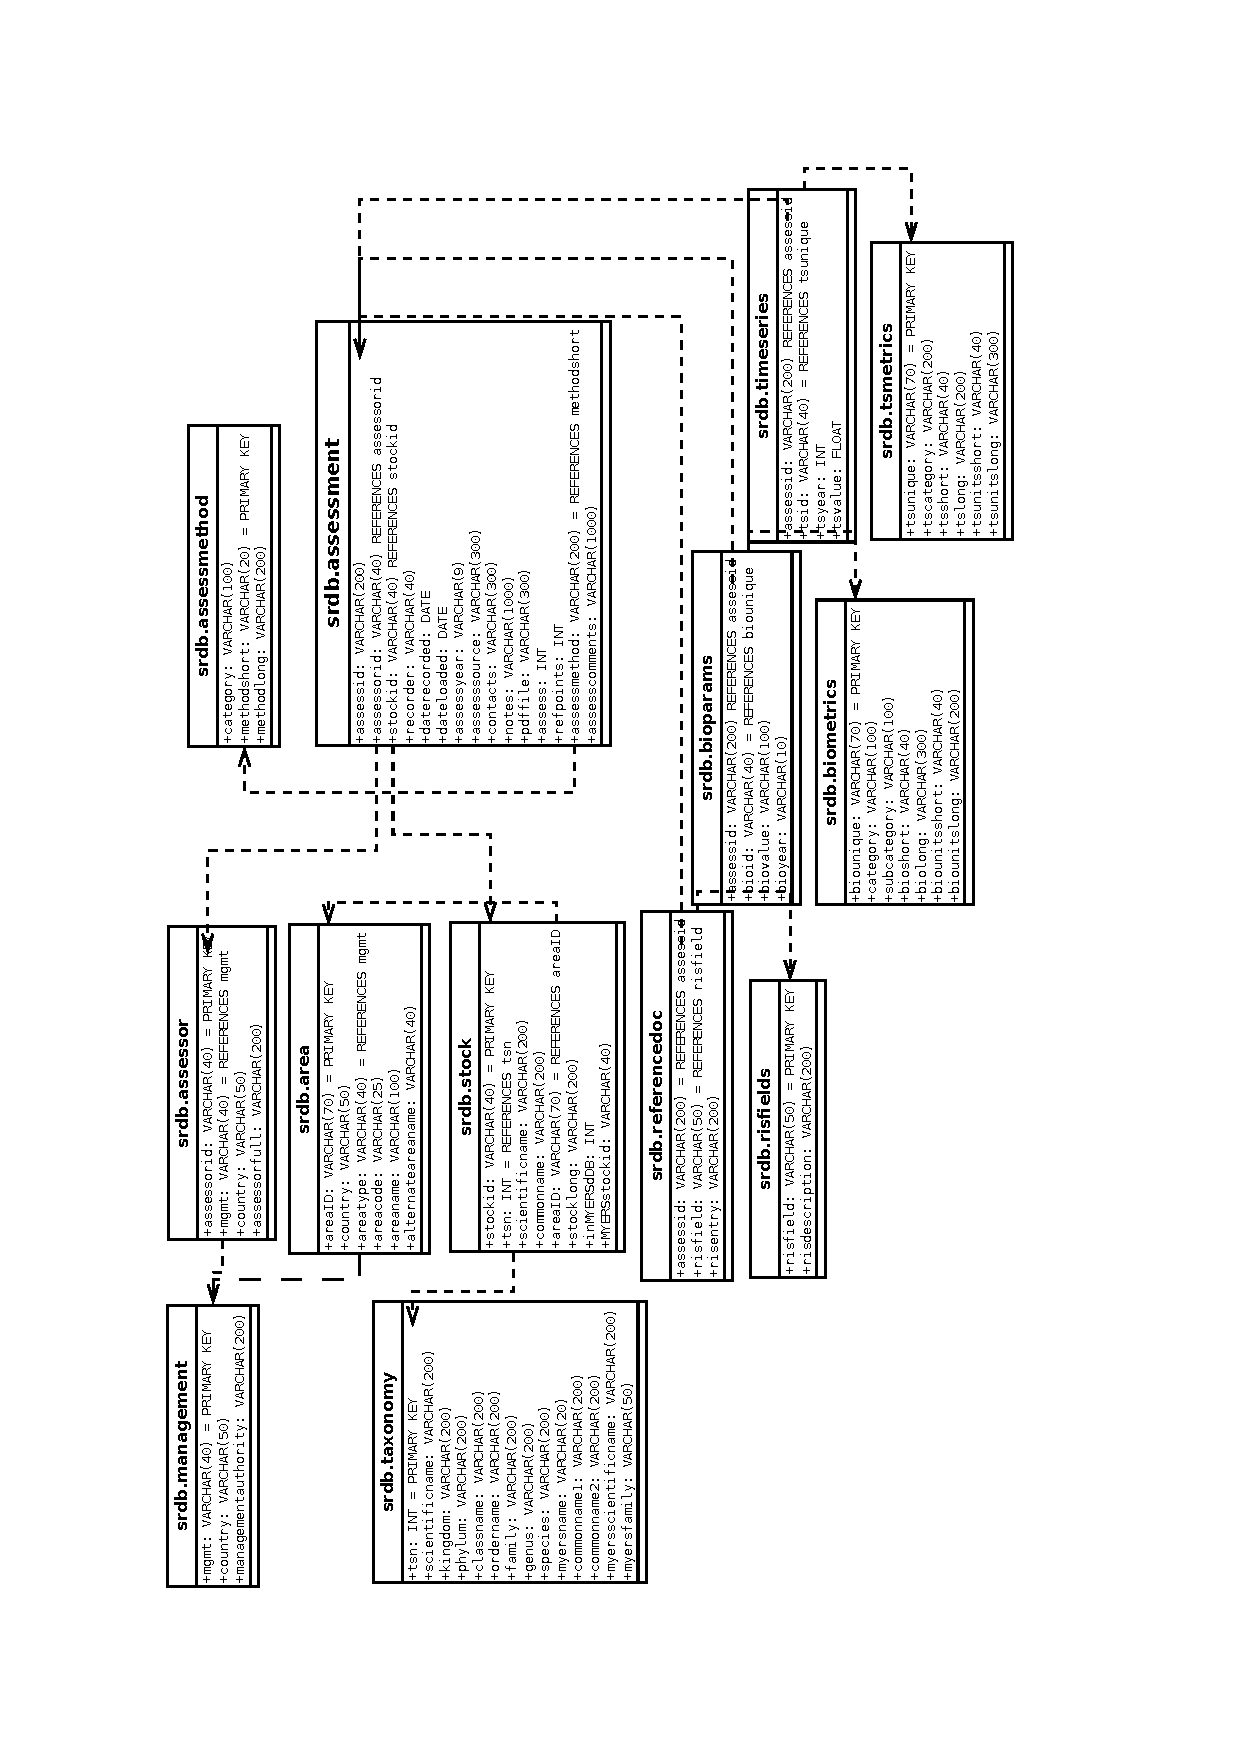
\includegraphics[width=15cm]{/home/srdbadmin/SQLpg/srdb/trunk/doc/srdb-ERD.pdf}
\end{center}
\caption{Entity relationship diagram of the RAM legacy database.}
\end{figure}


\begin{table}
\caption{Data used to generate Figure~\ref{fig:orca} - Summary of the assessments used in this analysis and the timespan of their different results. }
\begin{tabular}{| p{5cm} | p{3cm} | c | r  c  l | c | }\label{tab:timespan}
\textit{Fisheries stock} & \textit{Scientific name} & \textit{Timespan} & & \textit{Num. years available} & & \textit{Source} \\
 & & & Catch & SSB & R & \\
\hline \hline
blah & blah & 1970-2000 & 30 & 29 & 30 & (blah) \\
\end{tabular}
\end{table}


%\begin{table}
%\caption{Data used to generate Figures~\ref{fig:friedegg} and ~\ref{fig:friedeggmgmt} - Summary of the assessments used in this analysis and their estimated ratios of current biomass to the biomass at maximum sustainable yield and current harvest rate to the harvest rate that results is maximum sustainable yield. The estimated ratios were preferentially obtained directly from the assessment document or derived from surplus production model fits. When both an SSBmsy and Bmsy reference points are available, the SSB is chosen preferentially. }
%\begin{tabular}{| p{5cm} | p{3cm} | c | c | c | c | c |}\label{tab:crosshair}
%\textit{Fisheries stock} & \textit{Scientific name} & \textit{Current year} & \textit{B/Bmsy} & \textit{u/umsy} & \textit{From assessment?} & \textit{Source} \\
%\hline \hline
%blah & blah & 2000 & 1.0 & 1.0 & yes &  (blah) \\
%\end{tabular}
%\end{table}

% latex table generated in R 2.13.0 by xtable 1.5-6 package
% Thu May 19 14:38:14 2011
\begin{table}[ht]
\begin{center}
\begin{tabular}{ccc}
  \hline
 & SP U/Umsy $<$ 1 & SP U/Umsy $>$ 1 \\ 
  \hline
U/Umsy $<$ 1 &  20 &  14 \\ 
  U/Umsy $>$ 1 &   2 &   8 \\ 
  B/Bmsy $<$ 1 &  28 &   6 \\ 
  B/Bmsy $>$ 1 &  12 &  30 \\ 
   \hline
\end{tabular}
\caption{Contingency tables of stock status classification for biomass and exploitation reference points obtained from assessments and those derived from surplus production models. }
\label{tab:contingency}
\end{center}
\end{table}

\begin{table}[ht]
\begin{center}
\begin{tabular}{rllrrrl}
  \hline
 & stock & scientificname & currentyear & Bratio & Uratio & fromassessment \\
  \hline
1 & Alaska plaice Bering Sea and Aleutian Islands & Pleuronectes quadrituberculatus & 2008 & 2.46 & 0.05 & yes \\
  2 & Arrowtooth flounder Bering Sea and Aleutian Islands & Reinhardtius stomias & 2008 & 1.28 & 0.31 & no \\
  3 & Arrowtooth flounder Gulf of Alaska & Reinhardtius stomias & 2007 & 1.33 & 0.28 & no \\
  4 & Atka mackerel Bering Sea and Aleutian Islands & Pleurogrammus monopterygius & 2008 & 1.50 & 0.55 & no \\
  5 & Cabezon Northern California & Scorpaenichthys marmoratus & 2004 & 0.89 & 0.99 & no \\
  6 & Cabezon Southern California & Scorpaenichthys marmoratus & 2004 & 0.81 & 0.53 & no \\
  7 & Dusky rockfish Gulf of Alaska & Sebastes variabilis & 2007 & 1.54 & 0.54 & yes \\
  8 & Flathead sole Bering Sea and Aleutian Islands & Hippoglossoides elassodon & 2008 & 1.66 & 0.18 & no \\
  9 & Greenland turbot Bering Sea and Aleutian Islands & Reinhardtius hippoglossoides & 2009 & 1.48 & 0.05 & yes \\
  10 & Northern rockfish Bering Sea and Aleutian Islands & Sebastes polyspinis & 2008 & 1.07 & 0.13 & no \\
  11 & Northern rockfish Gulf of Alaska & Sebastes polyspinis & 2008 & 1.50 & 0.66 & yes \\
  12 & Northern rock sole Eastern Bering Sea and Aleutian Islands & Lepidopsetta polyxystra & 2007 & 3.02 & 0.21 & yes \\
  13 & Pacific cod Bering Sea and Aleutian Islands & Gadus macrocephalus & 2007 & 0.89 & 0.93 & no \\
  14 & Pacific cod Gulf of Alaska & Gadus macrocephalus & 2007 & 1.07 & 0.84 & no \\
  15 & Pacific Ocean perch Eastern Bering Sea and Aleutian Islands & Sebastes alutus & 2008 & 1.70 & 0.26 & no \\
  16 & Pacific ocean perch Gulf of Alaska & Sebastes alutus & 2008 & 1.16 & 0.73 & yes \\
  17 & Red king crab Bristol Bay & Paralithodes camtschaticus & 2007 & 0.00 & 1.38 & no \\
  18 & Sablefish Eastern Bering Sea / Aleutian Islands / Gulf of Alaska & Anoplopoma fimbria & 2008 & 0.72 & 0.90 & no \\
  19 & Snow crab Bering Sea & Chionoecetes opilio & 2008 & 0.29 & 1.61 & no \\
  20 & Walleye pollock Aleutian Islands & Theragra chalcogramma & 2008 & 0.86 & 0.02 & yes \\
  21 & Walleye pollock Eastern Bering Sea & Theragra chalcogramma & 2008 & 0.68 & 0.85 & no \\
  22 & Yellowfin sole Bering Sea and Aleutian Islands & Limanda aspera & 2008 & 1.94 & 0.62 & yes \\
  23 & Capelin Barents Sea & Mallotus villosus & 2006 & 0.17 & 0.00 & no \\
  24 & Atlantic cod coastal Norway & Gadus morhua & 2006 & 0.20 & 2.57 & no \\
  25 & Atlantic cod Northeast Arctic & Gadus morhua & 2006 & 0.56 & 1.42 & no \\
  26 & Greenland halibut Northeast Arctic & Reinhardtius hippoglossoides & 2006 & 0.23 & 1.38 & no \\
  27 & Golden Redfish Northeast Arctic & Sebastes norvegicus & 2006 & 0.00 & 4.25 & no \\
  28 & Haddock Northeast Arctic & Melanogrammus aeglefinus & 2006 & 1.10 & 1.06 & no \\
  29 & Pollock Northeast Arctic & Pollachius virens & 2006 & 1.70 & 0.60 & no \\
  30 & Atlantic croaker Mid-Atlantic Coast & Micropogonias undulatus & 2002 & 1.42 & 0.27 & yes \\
  31 & Northern shrimp Gulf of Maine & Pandalus borealis & 2008 & 1.58 & 0.56 & no \\
  32 & Antarctic toothfish Ross Sea & Dissostichus mawsoni & 2007 & 1.76 & 1.09 & no \\
  33 & Deepwater flathead Southeast Australia & Platycephalus conatus & 2006 & 1.33 & 0.61 & no \\
  34 & common gemfish Southeast Australia & Rexea solandri & 2007 & 0.01 & 0.59 & no \\
  35 & Jackass morwong Southeast Australia & Nemadactylus macropterus & 2007 & 0.25 & 1.80 & no \\
  36 & New Zealand ling Eastern half of Southeast Australia & Genypterus blacodes & 2007 & 0.60 & 2.20 & no \\
  37 & Orange roughy Cascade Plateau & Hoplostethus atlanticus & 2006 & 1.76 & 0.34 & no \\
  38 & Orange roughy Southeast Australia & Hoplostethus atlanticus & 2006 & 0.89 & 0.29 & no \\
  39 & Silverfish Southeast Australia & Seriolella punctata & 2006 & 1.15 & 0.79 & no \\
  40 & School whiting Southeast Australia & Sillago flindersi & 2007 & 1.10 & 0.82 & no \\
  41 & Tiger flathead Southeast Australia & Neoplatycephalus richardsoni & 2006 & 1.05 & 0.00 & no \\
  42 & Blue Warehou Eastern half of Southeast Australia & Seriolella brama & 2006 & 0.17 & 0.84 & no \\
  43 & Blue Warehou Western half of Southeast Australia & Seriolella brama & 2006 & 0.62 & 2.04 & no \\
  44 & Atlantic cod NAFO 5Zjm & Gadus morhua & 2002 & 0.00 & 0.74 & no \\
  45 & Haddock NAFO-4X5Y & Melanogrammus aeglefinus & 2003 & 0.28 & 0.45 & no \\
  46 & Haddock NAFO-5Zejm & Melanogrammus aeglefinus & 2002 & 0.15 & 0.86 & no \\
  47 & Atlantic cod NAFO 2J3KL inshore & Gadus morhua & 2005 & 1.60 & 0.14 & no \\
  48 & Atlantic cod NAFO 3Ps & Gadus morhua & 2004 & 0.43 & 0.43 & no \\
  49 & English sole Hecate Strait & Parophrys vetulus & 2001 & 1.23 & 0.37 & no \\
  50 & Pacific herring Central Coast & Clupea pallasii & 2007 & 0.30 & 0.11 & no \\
  51 & Pacific herring Prince Rupert District & Clupea pallasii & 2007 & 0.00 & 0.44 & no \\
  52 & Pacific herring Queen Charlotte Islands & Clupea pallasii & 2007 & 0.20 & 0.00 & no \\
  53 & Pacific herring Straight of Georgia & Clupea pallasii & 2007 & 0.91 & 0.40 & no \\
  54 & Pacific herring West Coast of Vancouver Island & Clupea pallasii & 2007 & 0.03 & 0.00 & no \\
  55 & Pacific cod Hecate Strait & Gadus macrocephalus & 2004 & 0.37 & 0.25 & no \\
  56 & Pacific cod West Coast of Vancouver Island & Gadus macrocephalus & 2001 & 0.28 & 0.61 & no \\
  57 & Rock sole Hecate Strait & Lepidopsetta bilineata & 2001 & 1.03 & 0.45 & no \\
  58 & Pollock NAFO-4VWX5Zc & Pollachius virens & 2006 & 0.56 & 0.30 & no \\
  59 & Atlantic cod NAFO 3Pn4RS & Gadus morhua & 2006 & 0.03 & 1.09 & no \\
  60 & Atlantic cod NAFO 4TVn & Gadus morhua & 2006 & 0.17 & 0.32 & no \\
  61 & Herring ICES 22-24-IIIa & Clupea harengus & 2006 & 0.73 & 1.02 & no \\
  62 & Herring Northern Irish Sea & Clupea harengus & 2006 & 0.72 & 0.34 & no \\
  63 & Herring North Sea & Clupea harengus & 2006 & 0.65 & 1.32 & no \\
  64 & Herring ICES VIa & Clupea harengus & 2006 & 0.18 & 1.59 & no \\
  65 & Herring ICES VIa-VIIb-VIIc & Clupea harengus & 2000 & 0.50 & 1.04 & no \\
  66 & Albacore tuna North Atlantic & Thunnus alalunga & 2005 & 0.81 & 1.49 & yes \\
  67 & Bluefin tuna Eastern Atlantic & Thunnus thynnus & 2007 & 0.34 & 9.38 & yes \\
  68 & Bluefin tuna Western Atlantic & Thunnus thynnus & 2007 & 0.57 & 1.33 & yes \\
  69 & Bigeye tuna Atlantic & Thunnus obesus & 2005 & 0.90 & 0.86 & no \\
  70 & Skipjack tuna Eastern Atlantic & Katsuwonus pelamis & 2006 & 1.71 & 0.27 & no \\
  71 & Skipjack tuna Western Atlantic & Katsuwonus pelamis & 2006 & 1.72 & 0.27 & no \\
  72 & Swordfish Mediterranean Sea & Xiphias gladius & 2006 & 0.94 & 1.27 & yes \\
  73 & Swordfish North Atlantic & Xiphias gladius & 2005 & 1.03 & 0.82 & no \\
  74 & Swordfish South Atlantic & Xiphias gladius & 2005 & 1.18 & 0.69 & no \\
  75 & Yellowfin tuna Atlantic & Thunnus albacares & 2006 & 1.07 & 0.81 & yes \\
  76 & Chilean jack mackerel Chilean EEZ and offshore & Trachurus murphyi & 2006 & 0.52 & 1.20 & no \\
  77 & Argentine anchoita Northern Argentina & Engraulis anchoita & 2007 & 1.37 & 0.17 & yes \\
  78 & Argentine anchoita Southern Argentina & Engraulis anchoita & 2007 & 3.13 & 0.04 & yes \\
  79 & Argentine hake Northern Argentina & Merluccius hubbsi & 2007 & 0.16 & 1.26 & yes \\
  80 & Argentine hake Southern Argentina & Merluccius hubbsi & 2008 & 0.34 & 1.49 & yes \\
  81 & Patagonian grenadier Southern Argentina & Macruronus magellanicus & 2006 & 1.82 & 0.60 & yes \\
  82 & Bigeye tuna Indian Ocean & Thunnus obesus & 2004 & 1.23 & 0.97 & yes \\
  83 & Pacific halibut North Pacific & Hippoglossus stenolepis & 2008 & 0.54 & 2.01 & no \\
  84 & Anchovy South Africa & Engraulis encrasicolus & 2006 & 0.97 & 0.36 & no \\
  85 & Shallow-water cape hake South Africa & Merluccius capensis & 2008 & 1.16 & 0.40 & no \\
  86 & Cape horse mackerel South Africa South coast & Trachurus capensis & 2007 & 1.47 & 0.76 & no \\
  87 & Kingklip South Africa & Engraulis encrasicolus & 2008 & 1.13 & 0.55 & no \\
  88 & Sardine South Africa & Sardinops sagax & 2006 & 0.75 & 0.55 & no \\
  89 & Southern spiny lobster South Africa South coast & Palinurus gilchristi & 2008 & 0.51 & 1.50 & no \\
  90 & American Plaice NAFO-3LNO & Hippoglossoides platessoides & 2006 & 0.02 & 1.05 & no \\
  91 & American Plaice NAFO-3M & Hippoglossoides platessoides & 2007 & 0.00 & 0.00 & no \\
  92 & Atlantic cod NAFO 3NO & Gadus morhua & 2006 & 0.00 & 0.38 & no \\
  93 & Greenland halibut NAFO 23KLMNO & Reinhardtius hippoglossoides & 2006 & 0.39 & 1.73 & no \\
  94 & Redfish species NAFO 3LN & Redfish species & 2008 & 1.88 & 0.04 & yes \\
  95 & Redfish species NAFO 3M & Redfish species & 2006 & 0.93 & 0.15 & no \\
  96 & Yellowtail Flounder NAFO 3LNO & Limanda ferruginea & 2007 & 1.62 & 0.15 & no \\
  97 & American Plaice NAFO-5YZ & Hippoglossoides platessoides & 2007 & 0.55 & 0.30 & no \\
  98 & Bluefish Atlantic Coast & Pomatomus saltatrix & 2007 & 0.81 & 1.25 & no \\
  99 & Black sea bass Mid-Atlantic Coast & Centropristis striata & 2007 & 1.21 & 0.67 & no \\
  100 & Atlantic cod Georges Bank & Gadus morhua & 2007 & 0.00 & 1.15 & no \\
  101 & Atlantic cod Gulf of Maine & Gadus morhua & 2007 & 1.46 & 0.29 & no \\
  102 & Haddock NAFO-5Y & Melanogrammus aeglefinus & 2007 & 0.00 & 1.86 & no \\
  103 & Monkfish Gulf of Maine / Northern Georges Bank & Lophius americanus & 2006 & 1.73 & 0.38 & no \\
  104 & Monkfish Southern Georges Bank / Mid-Atlantic & Lophius americanus & 2006 & 1.72 & 0.30 & no \\
  105 & Sea scallop Georges Bank & Placopecten magellanicus & 2006 & 1.59 & 0.78 & no \\
  106 & Sea scallop Mid-Atlantic Coast & Placopecten magellanicus & 2006 & 0.91 & 0.37 & no \\
  107 & Spiny dogfish Atlantic Coast & Squalus acanthias & 2005 & 1.61 & 0.15 & no \\
  108 & Atlantic surfclam Mid-Atlantic Coast & Spisula solidissima & 1994 & 1.85 & 0.00 & no \\
  109 & Tilefish Mid-Atlantic Coast & Lopholatilus chamaeleonticeps & 2005 & 0.72 & 0.61 & no \\
  110 & Weakfish Atlantic Coast & Cynoscion regalis & 2008 & 0.06 & 1.49 & no \\
  111 & White hake Georges Bank / Gulf of Maine & Urophycis tenuis & 2007 & 0.35 & 0.80 & yes \\
  112 & Winter Flounder NAFO-5Z & Pseudopleuronectes americanus & 2006 & 1.41 & 0.25 & no \\
  113 & Winter Flounder Southern New England-Mid Atlantic & Pseudopleuronectes americanus & 2007 & 0.07 & 1.44 & no \\
  114 & Witch Flounder NAFO-5Y & Glyptocephalus cynoglossus & 2007 & 0.30 & 1.45 & yes \\
  115 & Yellowtail flounder Cape Cod / Gulf of Maine & Limanda ferruginea & 2007 & 0.25 & 1.73 & yes \\
  116 & Yellowtail flounder Georges Bank & Limanda ferruginea & 2007 & 0.22 & 1.14 & yes \\
  117 & Yellowtail Flounder Southern New England-Mid Atlantic & Limanda ferruginea & 2007 & 0.13 & 1.61 & yes \\
  118 & Australian salmon New Zealand & Arripis trutta & 2006 & 1.64 & 0.33 & yes \\
  119 & Orange roughy New Zealand Mid East Coast & Hoplostethus atlanticus & 2004 & 1.20 & 0.35 & yes \\
  120 & Atlantic menhaden Atlantic & Brevoortia tyrannus & 2005 & 0.47 & 0.97 & no \\
  121 & Pacific sardine North Pacific & Sardinops sagax & 2006 & 1.73 & 0.37 & no \\
  122 & Arrowtooth flounder Pacific Coast & Reinhardtius stomias & 2007 & 3.81 & 0.21 & yes \\
  123 & Blackgill rockfish  Pacific Coast & Sebastes melanostomus & 2004 & 0.80 & 1.20 & no \\
  124 & Black rockfish Northern Pacific Coast & Sebastes melanops & 2006 & 1.37 & 0.57 & no \\
  125 & Black rockfish Southern Pacific Coast & Sebastes melanops & 2007 & 2.23 & 0.33 & yes \\
  126 & Blue rockfish California & Sebastes mystinus & 2007 & 0.75 & 1.19 & yes \\
  127 & Bocaccio Southern Pacific Coast & Sebastes paucispinis & 2006 & 0.32 & 0.10 & yes \\
  128 & Chilipepper Southern Pacific Coast & Sebastes goodei & 2006 & 1.43 & 0.04 & no \\
  129 & Cowcod Southern California & Sebastes levis & 2007 & 0.09 & 0.07 & yes \\
  130 & Canary rockfish Pacific Coast & Sebastes pinniger & 2007 & 0.85 & 0.02 & yes \\
  131 & Darkblotched rockfish Pacific Coast & Sebastes crameri & 2007 & 0.73 & 0.31 & yes \\
  132 & English sole Pacific Coast & Parophrys vetulus & 2006 & 2.06 & 0.14 & no \\
  133 & Longnose skate Pacific Coast & Raja rhina & 2007 & 1.56 & 0.40 & no \\
  134 & Longspine thornyhead Pacific Coast & Sebastolobus altivelis & 2005 & 2.65 & 0.23 & yes \\
  135 & Pacific hake Pacific Coast & Merluccius productus & 2007 & 0.42 & 1.67 & no \\
  136 & Pacific ocean perch Pacific Coast & Sebastes alutus & 2007 & 0.69 & 0.00 & yes \\
  137 & Petrale sole Northern Pacific Coast & Eopsetta jordani & 2004 & 0.96 & 1.26 & no \\
  138 & Petrale sole Southern Pacific Coast & Eopsetta jordani & 2004 & 0.63 & 0.61 & no \\
  139 & Sablefish Pacific Coast & Anoplopoma fimbria & 2007 & 0.84 & 1.09 & no \\
  140 & Shortspine thornyhead Pacific Coast & Sebastolobus alascanus & 2004 & 1.55 & 0.93 & no \\
  141 & Widow rockfish Pacific Coast & Sebastes entomelas & 2006 & 0.91 & 0.07 & no \\
  142 & Yelloweye rockfish Pacific Coast & Sebastes ruberrimus & 2006 & 0.38 & 0.34 & no \\
  143 & Yellowtail rockfish Northern Pacific Coast & Sebastes flavidus & 2005 & 0.75 & 0.51 & no \\
  144 & Capelin Iceland & Mallotus villosus & 2006 & 0.49 & 0.85 & no \\
  145 & Atlantic cod Faroe Plateau & Gadus morhua & 2006 & 0.26 & 1.52 & no \\
  146 & Atlantic cod Iceland & Gadus morhua & 2006 & 0.46 & 1.17 & no \\
  147 & Haddock Faroe Plateau & Melanogrammus aeglefinus & 2006 & 0.85 & 1.07 & no \\
  148 & Haddock Iceland & Melanogrammus aeglefinus & 2007 & 0.73 & 1.36 & no \\
  149 & Pollock Faroe Plateau & Pollachius virens & 2006 & 0.99 & 1.52 & no \\
  150 & Black oreo West end of Chatham Rise & Allocyttus niger & 2007 & 0.99 & 0.82 & yes \\
  151 & Smooth oreo Chatham Rise & Pseudocyttus maculatus & 2006 & 2.25 & 0.38 & yes \\
  152 & Smooth oreo West end of Chatham Rise & Pseudocyttus maculatus & 2004 & 1.25 & 0.53 & yes \\
  153 & Hoki Eastern New Zealand & Macruronus novaezelandiae & 2007 & 1.11 & 0.33 & no \\
  154 & Hoki Western New Zealand & Macruronus novaezelandiae & 2007 & 0.51 & 0.57 & no \\
  155 & New Zealand snapper New Zealand Area 8 & Chrysophrys auratus & 2005 & 0.35 & 2.50 & yes \\
  156 & Trevally New Zealand Areas TRE 7 & Pseudocaranx dentex & 2005 & 1.44 & 0.83 & yes \\
  157 & Red rock lobster New Zealand area CRA1 & Jasus edwardsii & 2001 & 1.14 & 0.88 & no \\
  158 & Red rock lobster New Zealand area CRA2 & Jasus edwardsii & 2001 & 0.53 & 2.12 & no \\
  159 & Red rock lobster New Zealand area CRA4 & Jasus edwardsii & 2005 & 0.67 & 1.33 & no \\
  160 & Red rock lobster New Zealand area CRA5 & Jasus edwardsii & 2002 & 0.59 & 1.68 & no \\
  161 & Red rock lobster New Zealand area CRA7 & Jasus edwardsii & 2005 & 0.73 & 0.43 & no \\
  162 & Red rock lobster New Zealand area CRA8 & Jasus edwardsii & 2005 & 0.69 & 0.49 & no \\
  163 & common gemfish New Zealand & Rexea solandri & 2006 & 1.64 & 0.43 & yes \\
  164 & New Zealand ling New Zealand Areas LIN 3 and 4 & Genypterus blacodes & 2007 & 3.07 & 0.09 & yes \\
  165 & New Zealand ling New Zealand Areas LIN 5 and 6 & Genypterus blacodes & 2007 & 3.96 & 0.10 & yes \\
  166 & New Zealand ling New Zealand Area LIN 6b & Genypterus blacodes & 2006 & 2.19 & 0.11 & yes \\
  167 & New Zealand ling New Zealand Area LIN 72 & Genypterus blacodes & 2007 & 2.49 & 0.32 & yes \\
  168 & New Zealand ling New Zealand Area LIN 7WC - WCSI & Genypterus blacodes & 2008 & 2.21 & 0.13 & yes \\
  169 & Southern blue whiting Campbell Island Rise & Micromesistius australis & 2006 & 1.15 & 0.92 & yes \\
  170 & Southern hake Chatham Rise & Merluccius australis & 2006 & 1.77 & 0.12 & yes \\
  171 & Southern hake Sub-Antarctic & Merluccius australis & 2007 & 2.91 & 0.11 & yes \\
  172 & New Zealand abalone species New Zealand Area PAU 5A & Haliotis iris & 2006 & 0.72 & 2.83 & no \\
  173 & New Zealand abalone species New Zealand Area PAU 5B & Haliotis iris & 2007 & 1.02 & 0.59 & no \\
  174 & New Zealand abalone species New Zealand Area PAU 5D & Haliotis iris & 2006 & 0.44 & 2.10 & no \\
  175 & New Zealand abalone species New Zealand Area PAU 7 & Haliotis iris & 2008 & 0.87 & 0.94 & no \\
  176 & American lobster Rhode Island & Homarus americanus & 2006 & 0.51 & 0.68 & no \\
  177 & Tautog Rhode Island & Tautoga onitis & 2006 & 0.84 & 0.59 & no \\
  178 & Winter flounder Rhode Island & Pseudopleuronectes americanus & 2006 & 0.03 & 2.35 & no \\
  179 & Gag Gulf of Mexico & Mycteroperca microlepis & 2004 & 1.25 & 1.84 & no \\
  180 & Gag Southern Atlantic coast & Mycteroperca microlepis & 2005 & 0.94 & 1.31 & yes \\
  181 & Greater amberjack Gulf of Mexico & Seriola dumerili & 2004 & 0.46 & 1.52 & no \\
  182 & King mackerel Gulf of Mexico & Scomberomorus cavalla & 2001 & 1.51 & 0.44 & no \\
  183 & King mackerel Southern Atlantic Coast & Scomberomorus cavalla & 2001 & 1.38 & 0.56 & no \\
  184 & Gulf menhaden Gulf of Mexico & Brevoortia patronus & 2004 & 1.08 & 0.48 & no \\
  185 & Red grouper Gulf of Mexico & Epinephelus morio & 2005 & 0.17 & 1.39 & no \\
  186 & Red porgy Southern Atlantic coast & Pagrus pagrus & 2004 & 0.61 & 0.39 & yes \\
  187 & Snowy grouper Southern Atlantic coast & Epinephelus niveatus & 2002 & 0.19 & 3.08 & yes \\
  188 & Spanish mackerel Southern Atlantic Coast & Scomberomorus maculatus & 2007 & 0.38 & 0.91 & yes \\
  189 & Tilefish Southern Atlantic coast & Lopholatilus chamaeleonticeps & 2002 & 0.94 & 1.55 & yes \\
  190 & Vermilion snapper Southern Atlantic coast & Rhomboplites aurorubens & 2007 & 0.86 & 1.27 & yes \\
  191 & Yellowtail snapper Southern Atlantic Coast and Gulf of Mexico & Ocyurus chrysurus & 2001 & 1.14 & 0.61 & yes \\
  192 & Walleye pollock Northern Sea of Okhotsk & Theragra chalcogramma & 1992 & 1.11 & 0.87 & no \\
  193 & Albacore tuna South Pacific Ocean & Thunnus alalunga & 2006 & 2.46 & 0.90 & yes \\
  194 & Bigeye tuna Western Pacific Ocean & Thunnus obesus & 2006 & 1.06 & 1.38 & yes \\
  195 & Skipjack tuna Central Western Pacific & Katsuwonus pelamis & 2006 & 4.38 & 0.30 & yes \\
  196 & Yellowfin tuna Central Western Pacific & Thunnus albacares & 2005 & 1.22 & 0.80 & yes \\
  197 & Dover sole Pacific Coast & Microstomus pacificus & 2004 & 1.33 & 0.45 & no \\
  198 & Gopher rockfish Southern Pacific Coast & Sebastes carnatus & 2004 & 1.69 & 0.08 & no \\
  199 & Pacific sardine Pacific Coast & Sardinops sagax & 2006 & 1.36 & 0.41 & no \\
  200 & Starry flounder Northern Pacific Coast & Platichthys stellatus & 2004 & 0.68 & 0.33 & no \\
  201 & Starry flounder Southern Pacific Coast & Platichthys stellatus & 2004 & 1.15 & 0.12 & no \\
  202 & Tasmanian giant crab Tasmania & Pseudocarcinus gigas & 2007 & 0.50 & 1.71 & no \\
  203 & Walleye pollock Western Bering Sea & Theragra chalcogramma & 2004 & 2.16 & 0.26 & no \\
  204 & Atlantic cod Baltic Areas 22 and 24 & Gadus morhua & 2006 & 0.31 & 1.55 & no \\
  205 & Atlantic cod Baltic Areas 25-32 & Gadus morhua & 2006 & 0.14 & 1.58 & no \\
  206 & Atlantic cod Kattegat & Gadus morhua & 2006 & 0.19 & 0.31 & no \\
  207 & Herring ICES 25-32 & Clupea harengus & 2006 & 0.69 & 0.79 & no \\
  208 & Herring ICES 30 & Clupea harengus & 2006 & 1.19 & 1.10 & no \\
  209 & Herring ICES 31 & Clupea harengus & 2006 & 0.27 & 1.65 & no \\
  210 & Herring Iceland (Summer spawners) & Clupea harengus & 2006 & 0.70 & 0.89 & no \\
  211 & Herring ICES 28 & Clupea harengus & 2006 & 1.21 & 0.87 & no \\
  212 & common European sole ICES Kattegat and Skagerrak & Solea vulgaris & 2006 & 1.25 & 0.54 & no \\
  213 & Sprat ICES Baltic Areas 22-32 & Sprattus sprattus & 2006 & 1.13 & 1.27 & no \\
  214 & Fourspotted megrim ICES VIIIc-IXa & Lepidorhombus boscii & 2006 & 0.00 & 1.61 & no \\
  215 & Hake Northeast Atlantic North & Merluccius merluccius & 2006 & 1.04 & 0.74 & no \\
  216 & Megrim ICES VIIIc-IXa & Lepidorhombus whiffiagonis & 2006 & 0.24 & 1.31 & no \\
  217 & common European sole Bay of Biscay & Solea vulgaris & 2006 & 0.62 & 1.13 & no \\
  218 & Mackerel ICES Northeast Atlantic & Scomber scombrus & 2006 & 0.98 & 0.73 & no \\
  219 & Whiting Northeast Atlantic & Micromesistius poutassou & 2006 & 0.67 & 1.66 & no \\
  220 & Atlantic cod Irish Sea & Gadus morhua & 2006 & 0.09 & 0.69 & no \\
  221 & Atlantic cod West of Scotland & Gadus morhua & 2006 & 0.10 & 0.45 & no \\
  222 & Haddock West of Scotland & Melanogrammus aeglefinus & 2006 & 0.58 & 0.73 & no \\
  223 & European Plaice Irish Sea & Pleuronectes platessa & 2006 & 1.07 & 0.23 & no \\
  224 & common European sole Irish Sea & Solea vulgaris & 2006 & 0.36 & 1.16 & no \\
  225 & Atlantic cod North Sea & Gadus morhua & 2006 & 0.19 & 0.80 & no \\
  226 & Haddock ICES IIIa and North Sea & Melanogrammus aeglefinus & 2006 & 0.62 & 0.25 & no \\
  227 & Haddock Rockall Bank & Melanogrammus aeglefinus & 2006 & 1.10 & 0.52 & no \\
  228 & Norway pout North Sea & Trisopterus esmarkii & 2006 & 0.90 & 0.33 & no \\
  229 & Pollock ICES IIIa, VI and North Sea & Pollachius virens & 2006 & 0.56 & 0.97 & no \\
  230 & Sandeel North Sea & Ammodytes marinus & 2007 & 0.92 & 0.24 & no \\
  231 & Whiting ICES IIIa, VIId and North Sea & Merlangius merlangus & 2006 & 0.33 & 1.04 & no \\
  232 & Haddock ICES VIIb-k & Melanogrammus aeglefinus & 2006 & 1.37 & 0.41 & no \\
  233 & European Plaice ICES VIIf-g & Pleuronectes platessa & 2006 & 0.65 & 0.41 & no \\
  234 & European Plaice ICES VIIe & Pleuronectes platessa & 2006 & 0.51 & 1.39 & no \\
  235 & common European sole Celtic Sea & Solea vulgaris & 2006 & 0.90 & 0.95 & no \\
  236 & common European sole Western English Channel & Solea vulgaris & 2006 & 0.51 & 1.75 & no \\
  237 & Whiting ICES VIIe-k & Merlangius merlangus & 2006 & 0.44 & 1.25 & no \\
   \hline
\end{tabular}
\caption{Data used to generate Figures~\ref{fig:friedegg} and ~\ref{fig:friedeggmgmt} - Summary of the assessments used in this analysis and their estimated ratios of current biomass to the biomass at maximum sustainable yield and current harvest rate to the harvest rate that results is maximum sustainable yield. The estimated ratios were preferentially obtained directly from the assessment document or derived from surplus production model fits. When both an SSBmsy and Bmsy reference points are available, the SSB is chosen preferentially.}
\label{tab:crosshair}
\end{center}
\end{table}


\end{document}

 % - open-ended, this is just the beginning, we want more assessments
